% Options for packages loaded elsewhere
\PassOptionsToPackage{unicode}{hyperref}
\PassOptionsToPackage{hyphens}{url}
%
\documentclass[
]{article}
\usepackage{amsmath,amssymb}
\usepackage{iftex}
\ifPDFTeX
  \usepackage[T1]{fontenc}
  \usepackage[utf8]{inputenc}
  \usepackage{textcomp} % provide euro and other symbols
\else % if luatex or xetex
  \usepackage{unicode-math} % this also loads fontspec
  \defaultfontfeatures{Scale=MatchLowercase}
  \defaultfontfeatures[\rmfamily]{Ligatures=TeX,Scale=1}
\fi
\usepackage{lmodern}
\ifPDFTeX\else
  % xetex/luatex font selection
\fi
% Use upquote if available, for straight quotes in verbatim environments
\IfFileExists{upquote.sty}{\usepackage{upquote}}{}
\IfFileExists{microtype.sty}{% use microtype if available
  \usepackage[]{microtype}
  \UseMicrotypeSet[protrusion]{basicmath} % disable protrusion for tt fonts
}{}
\makeatletter
\@ifundefined{KOMAClassName}{% if non-KOMA class
  \IfFileExists{parskip.sty}{%
    \usepackage{parskip}
  }{% else
    \setlength{\parindent}{0pt}
    \setlength{\parskip}{6pt plus 2pt minus 1pt}}
}{% if KOMA class
  \KOMAoptions{parskip=half}}
\makeatother
\usepackage{xcolor}
\usepackage[margin=1in]{geometry}
\usepackage{color}
\usepackage{fancyvrb}
\newcommand{\VerbBar}{|}
\newcommand{\VERB}{\Verb[commandchars=\\\{\}]}
\DefineVerbatimEnvironment{Highlighting}{Verbatim}{commandchars=\\\{\}}
% Add ',fontsize=\small' for more characters per line
\usepackage{framed}
\definecolor{shadecolor}{RGB}{248,248,248}
\newenvironment{Shaded}{\begin{snugshade}}{\end{snugshade}}
\newcommand{\AlertTok}[1]{\textcolor[rgb]{0.94,0.16,0.16}{#1}}
\newcommand{\AnnotationTok}[1]{\textcolor[rgb]{0.56,0.35,0.01}{\textbf{\textit{#1}}}}
\newcommand{\AttributeTok}[1]{\textcolor[rgb]{0.13,0.29,0.53}{#1}}
\newcommand{\BaseNTok}[1]{\textcolor[rgb]{0.00,0.00,0.81}{#1}}
\newcommand{\BuiltInTok}[1]{#1}
\newcommand{\CharTok}[1]{\textcolor[rgb]{0.31,0.60,0.02}{#1}}
\newcommand{\CommentTok}[1]{\textcolor[rgb]{0.56,0.35,0.01}{\textit{#1}}}
\newcommand{\CommentVarTok}[1]{\textcolor[rgb]{0.56,0.35,0.01}{\textbf{\textit{#1}}}}
\newcommand{\ConstantTok}[1]{\textcolor[rgb]{0.56,0.35,0.01}{#1}}
\newcommand{\ControlFlowTok}[1]{\textcolor[rgb]{0.13,0.29,0.53}{\textbf{#1}}}
\newcommand{\DataTypeTok}[1]{\textcolor[rgb]{0.13,0.29,0.53}{#1}}
\newcommand{\DecValTok}[1]{\textcolor[rgb]{0.00,0.00,0.81}{#1}}
\newcommand{\DocumentationTok}[1]{\textcolor[rgb]{0.56,0.35,0.01}{\textbf{\textit{#1}}}}
\newcommand{\ErrorTok}[1]{\textcolor[rgb]{0.64,0.00,0.00}{\textbf{#1}}}
\newcommand{\ExtensionTok}[1]{#1}
\newcommand{\FloatTok}[1]{\textcolor[rgb]{0.00,0.00,0.81}{#1}}
\newcommand{\FunctionTok}[1]{\textcolor[rgb]{0.13,0.29,0.53}{\textbf{#1}}}
\newcommand{\ImportTok}[1]{#1}
\newcommand{\InformationTok}[1]{\textcolor[rgb]{0.56,0.35,0.01}{\textbf{\textit{#1}}}}
\newcommand{\KeywordTok}[1]{\textcolor[rgb]{0.13,0.29,0.53}{\textbf{#1}}}
\newcommand{\NormalTok}[1]{#1}
\newcommand{\OperatorTok}[1]{\textcolor[rgb]{0.81,0.36,0.00}{\textbf{#1}}}
\newcommand{\OtherTok}[1]{\textcolor[rgb]{0.56,0.35,0.01}{#1}}
\newcommand{\PreprocessorTok}[1]{\textcolor[rgb]{0.56,0.35,0.01}{\textit{#1}}}
\newcommand{\RegionMarkerTok}[1]{#1}
\newcommand{\SpecialCharTok}[1]{\textcolor[rgb]{0.81,0.36,0.00}{\textbf{#1}}}
\newcommand{\SpecialStringTok}[1]{\textcolor[rgb]{0.31,0.60,0.02}{#1}}
\newcommand{\StringTok}[1]{\textcolor[rgb]{0.31,0.60,0.02}{#1}}
\newcommand{\VariableTok}[1]{\textcolor[rgb]{0.00,0.00,0.00}{#1}}
\newcommand{\VerbatimStringTok}[1]{\textcolor[rgb]{0.31,0.60,0.02}{#1}}
\newcommand{\WarningTok}[1]{\textcolor[rgb]{0.56,0.35,0.01}{\textbf{\textit{#1}}}}
\usepackage{graphicx}
\makeatletter
\def\maxwidth{\ifdim\Gin@nat@width>\linewidth\linewidth\else\Gin@nat@width\fi}
\def\maxheight{\ifdim\Gin@nat@height>\textheight\textheight\else\Gin@nat@height\fi}
\makeatother
% Scale images if necessary, so that they will not overflow the page
% margins by default, and it is still possible to overwrite the defaults
% using explicit options in \includegraphics[width, height, ...]{}
\setkeys{Gin}{width=\maxwidth,height=\maxheight,keepaspectratio}
% Set default figure placement to htbp
\makeatletter
\def\fps@figure{htbp}
\makeatother
\setlength{\emergencystretch}{3em} % prevent overfull lines
\providecommand{\tightlist}{%
  \setlength{\itemsep}{0pt}\setlength{\parskip}{0pt}}
\setcounter{secnumdepth}{-\maxdimen} % remove section numbering
\usepackage{fvextra} \DefineVerbatimEnvironment{Highlighting}{Verbatim}{breaklines,commandchars=\\\{\}} \usepackage{listings} \lstset{breaklines=true}
\ifLuaTeX
  \usepackage{selnolig}  % disable illegal ligatures
\fi
\IfFileExists{bookmark.sty}{\usepackage{bookmark}}{\usepackage{hyperref}}
\IfFileExists{xurl.sty}{\usepackage{xurl}}{} % add URL line breaks if available
\urlstyle{same}
\hypersetup{
  pdftitle={SIM. Assignment 2: Telco Customer Churn},
  pdfauthor={Adrià Casanova, Víctor Garcia, Zhengyong Ji},
  hidelinks,
  pdfcreator={LaTeX via pandoc}}

\title{SIM. Assignment 2: Telco Customer Churn}
\author{Adrià Casanova, Víctor Garcia, Zhengyong Ji}
\date{2024-01-05}

\begin{document}
\maketitle

{
\setcounter{tocdepth}{3}
\tableofcontents
}
\hypertarget{introduction}{%
\section{0. Introduction}\label{introduction}}

In this project, we will study the data set ``Telco Customer Churn'',
which can be found at
\url{https://www.kaggle.com/datasets/blastchar/telco-customer-churn}.
Our goal is to analyze the correlation between the amount of customers
who left within the last month (Churn) and different features that
describe the customer and the services he/she/they has signed up for.
Then, we will build a logistic model that will allow us to predict the
variable Churn.

All members have contributed equally to all parts of the project.

We start by taking a first general look at the dataset.

\begin{Shaded}
\begin{Highlighting}[]
\FunctionTok{head}\NormalTok{(df)}
\end{Highlighting}
\end{Shaded}

\begin{verbatim}
##   customerID gender SeniorCitizen Partner Dependents tenure PhoneService
## 1 7590-VHVEG Female             0     Yes         No      1           No
## 2 5575-GNVDE   Male             0      No         No     34          Yes
## 3 3668-QPYBK   Male             0      No         No      2          Yes
## 4 7795-CFOCW   Male             0      No         No     45           No
## 5 9237-HQITU Female             0      No         No      2          Yes
## 6 9305-CDSKC Female             0      No         No      8          Yes
##      MultipleLines InternetService OnlineSecurity OnlineBackup DeviceProtection
## 1 No phone service             DSL             No          Yes               No
## 2               No             DSL            Yes           No              Yes
## 3               No             DSL            Yes          Yes               No
## 4 No phone service             DSL            Yes           No              Yes
## 5               No     Fiber optic             No           No               No
## 6              Yes     Fiber optic             No           No              Yes
##   TechSupport StreamingTV StreamingMovies       Contract PaperlessBilling
## 1          No          No              No Month-to-month              Yes
## 2          No          No              No       One year               No
## 3          No          No              No Month-to-month              Yes
## 4         Yes          No              No       One year               No
## 5          No          No              No Month-to-month              Yes
## 6          No         Yes             Yes Month-to-month              Yes
##               PaymentMethod MonthlyCharges TotalCharges Churn
## 1          Electronic check          29.85        29.85    No
## 2              Mailed check          56.95      1889.50    No
## 3              Mailed check          53.85       108.15   Yes
## 4 Bank transfer (automatic)          42.30      1840.75    No
## 5          Electronic check          70.70       151.65   Yes
## 6          Electronic check          99.65       820.50   Yes
\end{verbatim}

\begin{Shaded}
\begin{Highlighting}[]
\FunctionTok{dim}\NormalTok{(df)}
\end{Highlighting}
\end{Shaded}

\begin{verbatim}
## [1] 7043   21
\end{verbatim}

\begin{Shaded}
\begin{Highlighting}[]
\FunctionTok{summary}\NormalTok{(df)}
\end{Highlighting}
\end{Shaded}

\begin{verbatim}
##       customerID      gender     SeniorCitizen    Partner    Dependents
##  0002-ORFBO:   1   Female:3488   Min.   :0.0000   No :3641   No :4933  
##  0003-MKNFE:   1   Male  :3555   1st Qu.:0.0000   Yes:3402   Yes:2110  
##  0004-TLHLJ:   1                 Median :0.0000                        
##  0011-IGKFF:   1                 Mean   :0.1621                        
##  0013-EXCHZ:   1                 3rd Qu.:0.0000                        
##  0013-MHZWF:   1                 Max.   :1.0000                        
##  (Other)   :7037                                                       
##      tenure      PhoneService          MultipleLines     InternetService
##  Min.   : 0.00   No : 682     No              :3390   DSL        :2421  
##  1st Qu.: 9.00   Yes:6361     No phone service: 682   Fiber optic:3096  
##  Median :29.00                Yes             :2971   No         :1526  
##  Mean   :32.37                                                          
##  3rd Qu.:55.00                                                          
##  Max.   :72.00                                                          
##                                                                         
##              OnlineSecurity              OnlineBackup 
##  No                 :3498   No                 :3088  
##  No internet service:1526   No internet service:1526  
##  Yes                :2019   Yes                :2429  
##                                                       
##                                                       
##                                                       
##                                                       
##             DeviceProtection              TechSupport  
##  No                 :3095    No                 :3473  
##  No internet service:1526    No internet service:1526  
##  Yes                :2422    Yes                :2044  
##                                                        
##                                                        
##                                                        
##                                                        
##               StreamingTV              StreamingMovies           Contract   
##  No                 :2810   No                 :2785   Month-to-month:3875  
##  No internet service:1526   No internet service:1526   One year      :1473  
##  Yes                :2707   Yes                :2732   Two year      :1695  
##                                                                             
##                                                                             
##                                                                             
##                                                                             
##  PaperlessBilling                   PaymentMethod  MonthlyCharges  
##  No :2872         Bank transfer (automatic):1544   Min.   : 18.25  
##  Yes:4171         Credit card (automatic)  :1522   1st Qu.: 35.50  
##                   Electronic check         :2365   Median : 70.35  
##                   Mailed check             :1612   Mean   : 64.76  
##                                                    3rd Qu.: 89.85  
##                                                    Max.   :118.75  
##                                                                    
##   TotalCharges    Churn     
##  Min.   :  18.8   No :5174  
##  1st Qu.: 401.4   Yes:1869  
##  Median :1397.5             
##  Mean   :2283.3             
##  3rd Qu.:3794.7             
##  Max.   :8684.8             
##  NA's   :11
\end{verbatim}

The data set contains 7043 observations of 21 variables.

\hypertarget{data-preparation}{%
\section{1. Data preparation}\label{data-preparation}}

The first part of the project consisted on doing some basic data
preparation to ensure that data is ready for the next sections.

Firstly, we checked that all datatypes were consistent with the metadata
and declared ``SeniorCitizen'' as a factor, as it represented a
qualitative concept.

\begin{Shaded}
\begin{Highlighting}[]
\NormalTok{df}\SpecialCharTok{$}\NormalTok{SeniorCitizen }\OtherTok{\textless{}{-}} \FunctionTok{factor}\NormalTok{(df}\SpecialCharTok{$}\NormalTok{SeniorCitizen, }\AttributeTok{labels =} \FunctionTok{c}\NormalTok{(}\StringTok{"Yes"}\NormalTok{,}
    \StringTok{"No"}\NormalTok{))}
\end{Highlighting}
\end{Shaded}

Secondly, we discretized all numeric variables by splitting data into 4
categories. Their boundaries were obtained simply by dividing the total
range in 4 equal intervals and the distribution was checked using
histograms to ensure that they were similar to the original variables.

\begin{Shaded}
\begin{Highlighting}[]
\NormalTok{df}\SpecialCharTok{$}\NormalTok{c.tenure }\OtherTok{\textless{}{-}}\NormalTok{ df}\SpecialCharTok{$}\NormalTok{tenure  }\CommentTok{\# Create a new variable called Categorical.tenure}
\NormalTok{m.tenure }\OtherTok{\textless{}{-}} \FunctionTok{max}\NormalTok{(df}\SpecialCharTok{$}\NormalTok{tenure, }\AttributeTok{na.rm =} \ConstantTok{TRUE}\NormalTok{)}
\NormalTok{df}\SpecialCharTok{$}\NormalTok{c.tenure }\OtherTok{\textless{}{-}} \FunctionTok{replace}\NormalTok{(df}\SpecialCharTok{$}\NormalTok{c.tenure, df}\SpecialCharTok{$}\NormalTok{tenure }\SpecialCharTok{\textless{}=}\NormalTok{ m.tenure}\SpecialCharTok{/}\DecValTok{4}\NormalTok{,}
\NormalTok{    m.tenure}\SpecialCharTok{/}\DecValTok{4}\NormalTok{)}
\ControlFlowTok{for}\NormalTok{ (i }\ControlFlowTok{in} \DecValTok{1}\SpecialCharTok{:}\DecValTok{3}\NormalTok{) \{}
\NormalTok{    idx }\OtherTok{\textless{}{-}}\NormalTok{ (m.tenure }\SpecialCharTok{*}\NormalTok{ i}\SpecialCharTok{/}\DecValTok{4} \SpecialCharTok{\textless{}}\NormalTok{ df}\SpecialCharTok{$}\NormalTok{tenure) }\SpecialCharTok{\&}\NormalTok{ (df}\SpecialCharTok{$}\NormalTok{tenure }\SpecialCharTok{\textless{}=}\NormalTok{ m.tenure }\SpecialCharTok{*}
\NormalTok{        (i }\SpecialCharTok{+} \DecValTok{1}\NormalTok{)}\SpecialCharTok{/}\DecValTok{4}\NormalTok{)}
\NormalTok{    df}\SpecialCharTok{$}\NormalTok{c.tenure }\OtherTok{\textless{}{-}} \FunctionTok{replace}\NormalTok{(df}\SpecialCharTok{$}\NormalTok{c.tenure, idx, m.tenure }\SpecialCharTok{*}\NormalTok{ (i }\SpecialCharTok{+}
        \DecValTok{1}\NormalTok{)}\SpecialCharTok{/}\DecValTok{4}\NormalTok{)}
\NormalTok{\}}
\FunctionTok{min}\NormalTok{(df}\SpecialCharTok{$}\NormalTok{tenure, }\AttributeTok{na.rm =} \ConstantTok{TRUE}\NormalTok{)}
\end{Highlighting}
\end{Shaded}

\begin{verbatim}
## [1] 0
\end{verbatim}

\begin{Shaded}
\begin{Highlighting}[]
\NormalTok{breakpts }\OtherTok{\textless{}{-}} \FunctionTok{seq}\NormalTok{(m.tenure}\SpecialCharTok{/}\DecValTok{4}\NormalTok{, m.tenure, m.tenure}\SpecialCharTok{/}\DecValTok{4}\NormalTok{)}
\NormalTok{breakpts}
\end{Highlighting}
\end{Shaded}

\begin{verbatim}
## [1] 18 36 54 72
\end{verbatim}

\begin{Shaded}
\begin{Highlighting}[]
\NormalTok{df}\SpecialCharTok{$}\NormalTok{c.tenure }\OtherTok{\textless{}{-}} \FunctionTok{factor}\NormalTok{(df}\SpecialCharTok{$}\NormalTok{c.tenure, }\AttributeTok{labels =} \FunctionTok{c}\NormalTok{(}\StringTok{"({-}1,18]"}\NormalTok{, }\StringTok{"(18,36]"}\NormalTok{,}
    \StringTok{"(36,54]"}\NormalTok{, }\StringTok{"(54,72]"}\NormalTok{))}
\FunctionTok{summary}\NormalTok{(df}\SpecialCharTok{$}\NormalTok{c.tenure)}
\end{Highlighting}
\end{Shaded}

\begin{verbatim}
## (-1,18] (18,36] (36,54] (54,72] 
##    2734    1308    1182    1819
\end{verbatim}

\begin{Shaded}
\begin{Highlighting}[]
\FunctionTok{par}\NormalTok{(}\AttributeTok{mfrow =} \FunctionTok{c}\NormalTok{(}\DecValTok{1}\NormalTok{, }\DecValTok{2}\NormalTok{))}
\FunctionTok{plot}\NormalTok{(df}\SpecialCharTok{$}\NormalTok{c.tenure, }\AttributeTok{main =} \StringTok{"Barplot of df$c.tenure"}\NormalTok{)}
\FunctionTok{hist}\NormalTok{(df}\SpecialCharTok{$}\NormalTok{tenure)}
\end{Highlighting}
\end{Shaded}

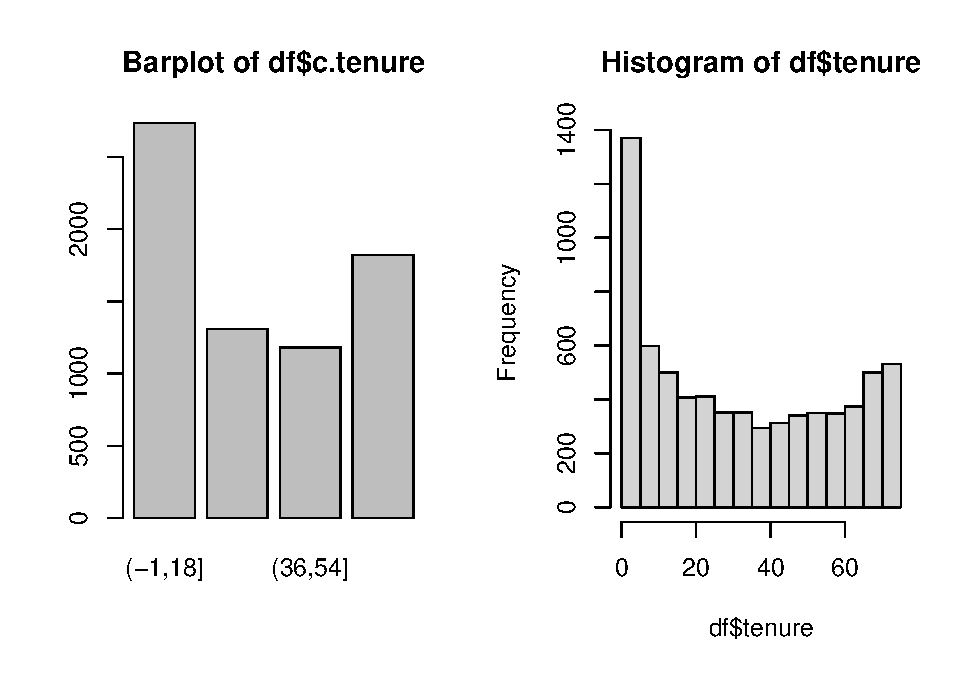
\includegraphics{AdriàCasanova-VíctorGarcia-ZhengyongJi_files/figure-latex/Discretize tenure-1.pdf}

\begin{Shaded}
\begin{Highlighting}[]
\NormalTok{df}\SpecialCharTok{$}\NormalTok{c.TotalCharges }\OtherTok{\textless{}{-}}\NormalTok{ df}\SpecialCharTok{$}\NormalTok{TotalCharges}
\NormalTok{m.TotalCharges }\OtherTok{\textless{}{-}} \FunctionTok{max}\NormalTok{(df}\SpecialCharTok{$}\NormalTok{TotalCharges, }\AttributeTok{na.rm =} \ConstantTok{TRUE}\NormalTok{)}
\NormalTok{df}\SpecialCharTok{$}\NormalTok{c.TotalCharges }\OtherTok{\textless{}{-}} \FunctionTok{replace}\NormalTok{(df}\SpecialCharTok{$}\NormalTok{c.TotalCharges, df}\SpecialCharTok{$}\NormalTok{TotalCharges }\SpecialCharTok{\textless{}=}
\NormalTok{    m.TotalCharges}\SpecialCharTok{/}\DecValTok{4}\NormalTok{, m.TotalCharges}\SpecialCharTok{/}\DecValTok{4}\NormalTok{)}
\ControlFlowTok{for}\NormalTok{ (i }\ControlFlowTok{in} \DecValTok{1}\SpecialCharTok{:}\DecValTok{3}\NormalTok{) \{}
\NormalTok{    idx }\OtherTok{\textless{}{-}}\NormalTok{ (m.TotalCharges }\SpecialCharTok{*}\NormalTok{ i}\SpecialCharTok{/}\DecValTok{4} \SpecialCharTok{\textless{}}\NormalTok{ df}\SpecialCharTok{$}\NormalTok{TotalCharges) }\SpecialCharTok{\&}\NormalTok{ (df}\SpecialCharTok{$}\NormalTok{TotalCharges }\SpecialCharTok{\textless{}=}
\NormalTok{        m.TotalCharges }\SpecialCharTok{*}\NormalTok{ (i }\SpecialCharTok{+} \DecValTok{1}\NormalTok{)}\SpecialCharTok{/}\DecValTok{4}\NormalTok{)}
\NormalTok{    df}\SpecialCharTok{$}\NormalTok{c.TotalCharges }\OtherTok{\textless{}{-}} \FunctionTok{replace}\NormalTok{(df}\SpecialCharTok{$}\NormalTok{c.TotalCharges, idx, m.TotalCharges }\SpecialCharTok{*}
\NormalTok{        (i }\SpecialCharTok{+} \DecValTok{1}\NormalTok{)}\SpecialCharTok{/}\DecValTok{4}\NormalTok{)}
\NormalTok{\}}
\NormalTok{breakpts }\OtherTok{\textless{}{-}} \FunctionTok{seq}\NormalTok{(m.TotalCharges}\SpecialCharTok{/}\DecValTok{4}\NormalTok{, m.TotalCharges, m.TotalCharges}\SpecialCharTok{/}\DecValTok{4}\NormalTok{)}
\NormalTok{breakpts}
\end{Highlighting}
\end{Shaded}

\begin{verbatim}
## [1] 2171.2 4342.4 6513.6 8684.8
\end{verbatim}

\begin{Shaded}
\begin{Highlighting}[]
\NormalTok{df}\SpecialCharTok{$}\NormalTok{c.TotalCharges }\OtherTok{\textless{}{-}} \FunctionTok{factor}\NormalTok{(df}\SpecialCharTok{$}\NormalTok{c.TotalCharges, }\AttributeTok{labels =} \FunctionTok{c}\NormalTok{(}\StringTok{"({-}1,2171]"}\NormalTok{,}
    \StringTok{"(2171,4342]"}\NormalTok{, }\StringTok{"(4342,6514]"}\NormalTok{, }\StringTok{"(6514,8685]"}\NormalTok{))}
\FunctionTok{summary}\NormalTok{(df}\SpecialCharTok{$}\NormalTok{c.TotalCharges)}
\end{Highlighting}
\end{Shaded}

\begin{verbatim}
##   (-1,2171] (2171,4342] (4342,6514] (6514,8685]        NA's 
##        4295        1270         975         492          11
\end{verbatim}

\begin{Shaded}
\begin{Highlighting}[]
\FunctionTok{par}\NormalTok{(}\AttributeTok{mfrow =} \FunctionTok{c}\NormalTok{(}\DecValTok{1}\NormalTok{, }\DecValTok{2}\NormalTok{))}
\FunctionTok{plot}\NormalTok{(df}\SpecialCharTok{$}\NormalTok{c.TotalCharges, }\AttributeTok{main =} \StringTok{"Barplot of df$c.TotalCharges"}\NormalTok{)}
\FunctionTok{hist}\NormalTok{(df}\SpecialCharTok{$}\NormalTok{TotalCharges)}
\end{Highlighting}
\end{Shaded}

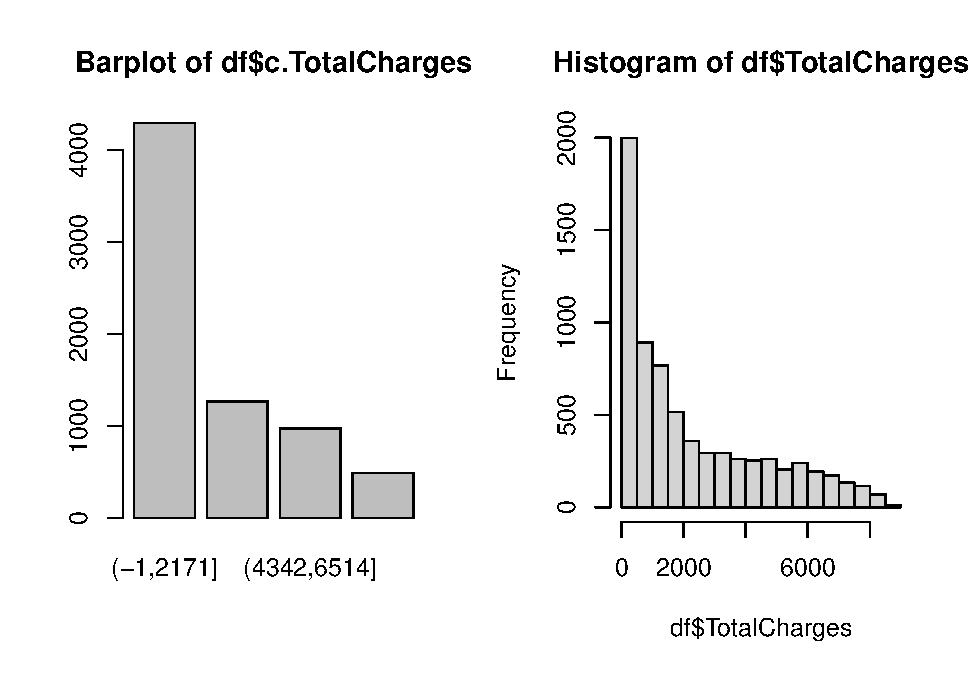
\includegraphics{AdriàCasanova-VíctorGarcia-ZhengyongJi_files/figure-latex/Discretize TotalCharges-1.pdf}

\begin{Shaded}
\begin{Highlighting}[]
\NormalTok{df}\SpecialCharTok{$}\NormalTok{c.MonthlyCharges }\OtherTok{\textless{}{-}}\NormalTok{ df}\SpecialCharTok{$}\NormalTok{MonthlyCharges}
\NormalTok{m.MonthlyCharges }\OtherTok{\textless{}{-}} \FunctionTok{max}\NormalTok{(df}\SpecialCharTok{$}\NormalTok{MonthlyCharges, }\AttributeTok{na.rm =} \ConstantTok{TRUE}\NormalTok{)}
\NormalTok{df}\SpecialCharTok{$}\NormalTok{c.MonthlyCharges }\OtherTok{\textless{}{-}} \FunctionTok{replace}\NormalTok{(df}\SpecialCharTok{$}\NormalTok{c.MonthlyCharges, df}\SpecialCharTok{$}\NormalTok{MonthlyCharges }\SpecialCharTok{\textless{}=}
\NormalTok{    m.MonthlyCharges}\SpecialCharTok{/}\DecValTok{4}\NormalTok{, m.MonthlyCharges}\SpecialCharTok{/}\DecValTok{4}\NormalTok{)}
\ControlFlowTok{for}\NormalTok{ (i }\ControlFlowTok{in} \DecValTok{1}\SpecialCharTok{:}\DecValTok{3}\NormalTok{) \{}
\NormalTok{    idx }\OtherTok{\textless{}{-}}\NormalTok{ (m.MonthlyCharges }\SpecialCharTok{*}\NormalTok{ i}\SpecialCharTok{/}\DecValTok{4} \SpecialCharTok{\textless{}}\NormalTok{ df}\SpecialCharTok{$}\NormalTok{MonthlyCharges) }\SpecialCharTok{\&}\NormalTok{ (df}\SpecialCharTok{$}\NormalTok{MonthlyCharges }\SpecialCharTok{\textless{}=}
\NormalTok{        m.MonthlyCharges }\SpecialCharTok{*}\NormalTok{ (i }\SpecialCharTok{+} \DecValTok{1}\NormalTok{)}\SpecialCharTok{/}\DecValTok{4}\NormalTok{)}
\NormalTok{    df}\SpecialCharTok{$}\NormalTok{c.MonthlyCharges }\OtherTok{\textless{}{-}} \FunctionTok{replace}\NormalTok{(df}\SpecialCharTok{$}\NormalTok{c.MonthlyCharges, idx,}
\NormalTok{        m.MonthlyCharges }\SpecialCharTok{*}\NormalTok{ (i }\SpecialCharTok{+} \DecValTok{1}\NormalTok{)}\SpecialCharTok{/}\DecValTok{4}\NormalTok{)}
\NormalTok{\}}
\FunctionTok{min}\NormalTok{(df}\SpecialCharTok{$}\NormalTok{MonthlyCharges, }\AttributeTok{na.rm =} \ConstantTok{TRUE}\NormalTok{)}
\end{Highlighting}
\end{Shaded}

\begin{verbatim}
## [1] 18.25
\end{verbatim}

\begin{Shaded}
\begin{Highlighting}[]
\NormalTok{breakpts }\OtherTok{\textless{}{-}} \FunctionTok{seq}\NormalTok{(m.MonthlyCharges}\SpecialCharTok{/}\DecValTok{4}\NormalTok{, m.MonthlyCharges, m.MonthlyCharges}\SpecialCharTok{/}\DecValTok{4}\NormalTok{)}
\NormalTok{breakpts}
\end{Highlighting}
\end{Shaded}

\begin{verbatim}
## [1]  29.6875  59.3750  89.0625 118.7500
\end{verbatim}

\begin{Shaded}
\begin{Highlighting}[]
\NormalTok{df}\SpecialCharTok{$}\NormalTok{c.MonthlyCharges }\OtherTok{\textless{}{-}} \FunctionTok{factor}\NormalTok{(df}\SpecialCharTok{$}\NormalTok{c.MonthlyCharges, }\AttributeTok{labels =} \FunctionTok{c}\NormalTok{(}\StringTok{"(18,30.69]"}\NormalTok{,}
    \StringTok{"(30.69,59.38]"}\NormalTok{, }\StringTok{"(59.38,89.06]"}\NormalTok{, }\StringTok{"(89.06,118.75]"}\NormalTok{))}
\FunctionTok{summary}\NormalTok{(df}\SpecialCharTok{$}\NormalTok{c.MonthlyCharges)}
\end{Highlighting}
\end{Shaded}

\begin{verbatim}
##     (18,30.69]  (30.69,59.38]  (59.38,89.06] (89.06,118.75] 
##           1634           1208           2317           1884
\end{verbatim}

\begin{Shaded}
\begin{Highlighting}[]
\FunctionTok{par}\NormalTok{(}\AttributeTok{mfrow =} \FunctionTok{c}\NormalTok{(}\DecValTok{1}\NormalTok{, }\DecValTok{2}\NormalTok{))}
\FunctionTok{plot}\NormalTok{(df}\SpecialCharTok{$}\NormalTok{c.MonthlyCharges, }\AttributeTok{main =} \StringTok{"Barplot of df$c.MonthlyCharges"}\NormalTok{)}
\FunctionTok{hist}\NormalTok{(df}\SpecialCharTok{$}\NormalTok{MonthlyCharges)}
\end{Highlighting}
\end{Shaded}

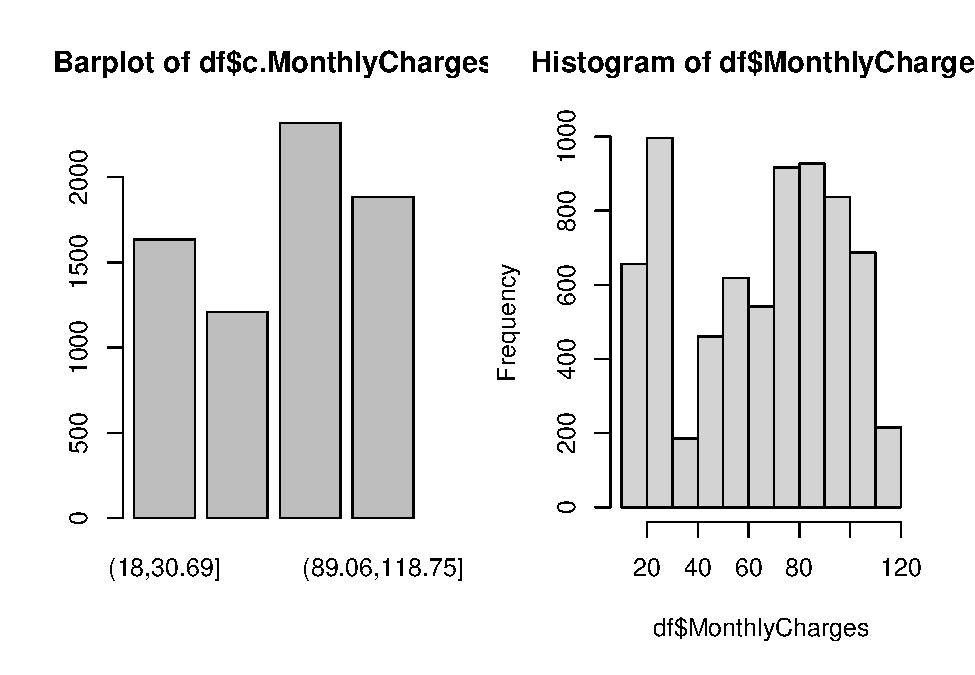
\includegraphics{AdriàCasanova-VíctorGarcia-ZhengyongJi_files/figure-latex/Discretize MonthlyCharges-1.pdf}

\begin{Shaded}
\begin{Highlighting}[]
\FunctionTok{par}\NormalTok{(}\AttributeTok{mfrow =} \FunctionTok{c}\NormalTok{(}\DecValTok{1}\NormalTok{, }\DecValTok{1}\NormalTok{))}
\end{Highlighting}
\end{Shaded}

Lastly, we identified categorical and numerical variables for later use.

\begin{Shaded}
\begin{Highlighting}[]
\NormalTok{numeric\_val\_idx }\OtherTok{=} \FunctionTok{which}\NormalTok{(}\FunctionTok{sapply}\NormalTok{(df, is.numeric))}
\NormalTok{numeric\_val }\OtherTok{=} \FunctionTok{names}\NormalTok{(df)[numeric\_val\_idx]}
\CommentTok{\# The only numerical features that we have are tenure,}
\CommentTok{\# MonthlyCharges and TotalChages.}

\CommentTok{\# So the remaining will be categorical features.}
\NormalTok{categoric\_val\_idx }\OtherTok{=} \FunctionTok{which}\NormalTok{(}\FunctionTok{sapply}\NormalTok{(df, is.factor))}
\NormalTok{categoric\_val }\OtherTok{=} \FunctionTok{names}\NormalTok{(df)[categoric\_val\_idx]}
\end{Highlighting}
\end{Shaded}

\hypertarget{exploratory-data-analysis-eda}{%
\section{2. Exploratory Data Analysis
(EDA)}\label{exploratory-data-analysis-eda}}

EDA was done mainly automatically using the ``DataExplorer'' library. It
plots, for each variable, the distribution of numeric variables, the
proportion of individuals in each category and the amount of missing
values, among other metadata.

The main conclusions of this section are: 1- Using the QQ plots and
distribution plots we see that no numerical variable is normally
distributed. This was also checked visually and with Kolmogorov-Smirnov
tests, a more suitable approach than Shappiro-Wilk for large samples.

2- Our database is not balanced in some categories, like PhoneService
(10\% of ``No'') or SeniorCitizen(16\% of ``No''). This is specially
relevant for the target, ``Churn'', that has 73\% of cases of ``No'', so
individuals that churned will be more difficult to predict.

3- Qualitative variables have a maximum of 4 levels, so all of them may
be suitable for modeling without any aggregation.

5- Some categories, like ``OnlineSecurity'' or ``OnlineBackup'', are not
applicable if the client does not have an internet connection.
Consequently, there is a special level for those cases that contains
around 22\% of the clients.

\begin{Shaded}
\begin{Highlighting}[]
\CommentTok{\# Basic EDA}
\FunctionTok{summary}\NormalTok{(df)}
\end{Highlighting}
\end{Shaded}

\begin{verbatim}
##       customerID      gender     SeniorCitizen Partner    Dependents
##  0002-ORFBO:   1   Female:3488   Yes:5901      No :3641   No :4933  
##  0003-MKNFE:   1   Male  :3555   No :1142      Yes:3402   Yes:2110  
##  0004-TLHLJ:   1                                                    
##  0011-IGKFF:   1                                                    
##  0013-EXCHZ:   1                                                    
##  0013-MHZWF:   1                                                    
##  (Other)   :7037                                                    
##      tenure      PhoneService          MultipleLines     InternetService
##  Min.   : 0.00   No : 682     No              :3390   DSL        :2421  
##  1st Qu.: 9.00   Yes:6361     No phone service: 682   Fiber optic:3096  
##  Median :29.00                Yes             :2971   No         :1526  
##  Mean   :32.37                                                          
##  3rd Qu.:55.00                                                          
##  Max.   :72.00                                                          
##                                                                         
##              OnlineSecurity              OnlineBackup 
##  No                 :3498   No                 :3088  
##  No internet service:1526   No internet service:1526  
##  Yes                :2019   Yes                :2429  
##                                                       
##                                                       
##                                                       
##                                                       
##             DeviceProtection              TechSupport  
##  No                 :3095    No                 :3473  
##  No internet service:1526    No internet service:1526  
##  Yes                :2422    Yes                :2044  
##                                                        
##                                                        
##                                                        
##                                                        
##               StreamingTV              StreamingMovies           Contract   
##  No                 :2810   No                 :2785   Month-to-month:3875  
##  No internet service:1526   No internet service:1526   One year      :1473  
##  Yes                :2707   Yes                :2732   Two year      :1695  
##                                                                             
##                                                                             
##                                                                             
##                                                                             
##  PaperlessBilling                   PaymentMethod  MonthlyCharges  
##  No :2872         Bank transfer (automatic):1544   Min.   : 18.25  
##  Yes:4171         Credit card (automatic)  :1522   1st Qu.: 35.50  
##                   Electronic check         :2365   Median : 70.35  
##                   Mailed check             :1612   Mean   : 64.76  
##                                                    3rd Qu.: 89.85  
##                                                    Max.   :118.75  
##                                                                    
##   TotalCharges    Churn         c.tenure        c.TotalCharges
##  Min.   :  18.8   No :5174   (-1,18]:2734   (-1,2171]  :4295  
##  1st Qu.: 401.4   Yes:1869   (18,36]:1308   (2171,4342]:1270  
##  Median :1397.5              (36,54]:1182   (4342,6514]: 975  
##  Mean   :2283.3              (54,72]:1819   (6514,8685]: 492  
##  3rd Qu.:3794.7                             NA's       :  11  
##  Max.   :8684.8                                               
##  NA's   :11                                                   
##        c.MonthlyCharges
##  (18,30.69]    :1634   
##  (30.69,59.38] :1208   
##  (59.38,89.06] :2317   
##  (89.06,118.75]:1884   
##                        
##                        
## 
\end{verbatim}

\begin{Shaded}
\begin{Highlighting}[]
\CommentTok{\# Complete EDA create\_report(df, output\_format =}
\CommentTok{\# \textquotesingle{}pdf\_document\textquotesingle{}, output\_file = \textquotesingle{}Telco.pdf\textquotesingle{})}
\end{Highlighting}
\end{Shaded}

\begin{Shaded}
\begin{Highlighting}[]
\CommentTok{\# tests}
\FunctionTok{ks.test}\NormalTok{(df}\SpecialCharTok{$}\NormalTok{TotalCharges, }\StringTok{"pnorm"}\NormalTok{)}
\end{Highlighting}
\end{Shaded}

\begin{verbatim}
## Warning in ks.test.default(df$TotalCharges, "pnorm"): Kolmogorov -
## Smirnov检验里不应该有连结
\end{verbatim}

\begin{verbatim}
## 
##  Asymptotic one-sample Kolmogorov-Smirnov test
## 
## data:  df$TotalCharges
## D = 1, p-value < 2.2e-16
## alternative hypothesis: two-sided
\end{verbatim}

\begin{Shaded}
\begin{Highlighting}[]
\FunctionTok{ks.test}\NormalTok{(df}\SpecialCharTok{$}\NormalTok{MonthlyCharges, }\StringTok{"pnorm"}\NormalTok{)}
\end{Highlighting}
\end{Shaded}

\begin{verbatim}
## Warning in ks.test.default(df$MonthlyCharges, "pnorm"): Kolmogorov -
## Smirnov检验里不应该有连结
\end{verbatim}

\begin{verbatim}
## 
##  Asymptotic one-sample Kolmogorov-Smirnov test
## 
## data:  df$MonthlyCharges
## D = 1, p-value < 2.2e-16
## alternative hypothesis: two-sided
\end{verbatim}

\begin{Shaded}
\begin{Highlighting}[]
\FunctionTok{ks.test}\NormalTok{(df}\SpecialCharTok{$}\NormalTok{tenure, }\StringTok{"pnorm"}\NormalTok{)}
\end{Highlighting}
\end{Shaded}

\begin{verbatim}
## Warning in ks.test.default(df$tenure, "pnorm"): Kolmogorov -
## Smirnov检验里不应该有连结
\end{verbatim}

\begin{verbatim}
## 
##  Asymptotic one-sample Kolmogorov-Smirnov test
## 
## data:  df$tenure
## D = 0.88865, p-value < 2.2e-16
## alternative hypothesis: two-sided
\end{verbatim}

\begin{Shaded}
\begin{Highlighting}[]
\CommentTok{\# plots}
\FunctionTok{par}\NormalTok{(}\AttributeTok{mfrow =} \FunctionTok{c}\NormalTok{(}\DecValTok{1}\NormalTok{, }\DecValTok{2}\NormalTok{))}
\FunctionTok{hist}\NormalTok{(df}\SpecialCharTok{$}\NormalTok{tenure, }\AttributeTok{prob =} \ConstantTok{TRUE}\NormalTok{, }\AttributeTok{breaks =} \DecValTok{10}\NormalTok{, }\AttributeTok{main =} \StringTok{"Histogram of tenure }
\StringTok{     vs normal distribution"}\NormalTok{,}
    \AttributeTok{xlab =} \StringTok{"tenure"}\NormalTok{)}
\NormalTok{x }\OtherTok{\textless{}{-}} \FunctionTok{seq}\NormalTok{(}\FunctionTok{min}\NormalTok{(df}\SpecialCharTok{$}\NormalTok{tenure), }\FunctionTok{max}\NormalTok{(df}\SpecialCharTok{$}\NormalTok{tenure), }\AttributeTok{by =} \FloatTok{0.1}\NormalTok{)}
\NormalTok{y }\OtherTok{\textless{}{-}} \FunctionTok{dnorm}\NormalTok{(x, }\AttributeTok{mean =} \FunctionTok{mean}\NormalTok{(df}\SpecialCharTok{$}\NormalTok{tenure), }\AttributeTok{sd =} \FunctionTok{sd}\NormalTok{(df}\SpecialCharTok{$}\NormalTok{tenure))}
\FunctionTok{plot}\NormalTok{(x, y, }\AttributeTok{xlab =} \StringTok{"tenuere"}\NormalTok{, }\AttributeTok{ylab =} \StringTok{""}\NormalTok{)}
\end{Highlighting}
\end{Shaded}

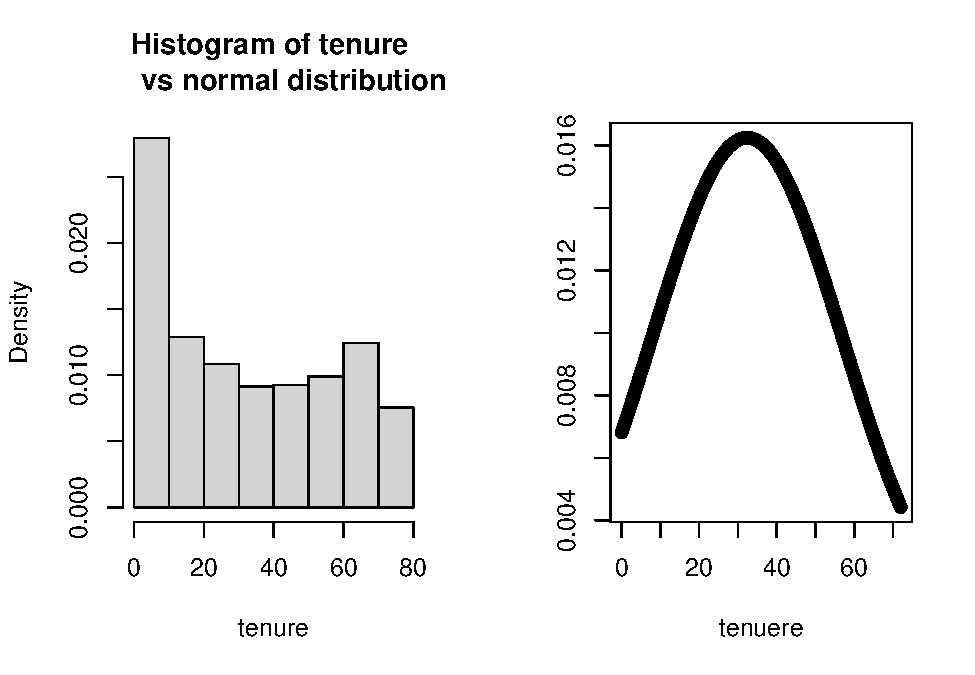
\includegraphics{AdriàCasanova-VíctorGarcia-ZhengyongJi_files/figure-latex/Analysis of normality-1.pdf}

\begin{Shaded}
\begin{Highlighting}[]
\FunctionTok{hist}\NormalTok{(df}\SpecialCharTok{$}\NormalTok{TotalCharges, }\AttributeTok{prob =} \ConstantTok{TRUE}\NormalTok{, }\AttributeTok{breaks =} \DecValTok{10}\NormalTok{, }\AttributeTok{main =} \StringTok{"Hist totalCharges }
\StringTok{     vs normal distribution"}\NormalTok{,}
    \AttributeTok{xlab =} \StringTok{"TotalCharges"}\NormalTok{)}
\NormalTok{x }\OtherTok{\textless{}{-}} \FunctionTok{seq}\NormalTok{(}\FunctionTok{min}\NormalTok{(df}\SpecialCharTok{$}\NormalTok{TotalCharges, }\AttributeTok{na.rm =} \ConstantTok{TRUE}\NormalTok{), }\FunctionTok{max}\NormalTok{(df}\SpecialCharTok{$}\NormalTok{TotalCharges,}
    \AttributeTok{na.rm =} \ConstantTok{TRUE}\NormalTok{), }\AttributeTok{by =} \DecValTok{10}\NormalTok{)}
\NormalTok{y }\OtherTok{\textless{}{-}} \FunctionTok{dnorm}\NormalTok{(x, }\AttributeTok{mean =} \FunctionTok{mean}\NormalTok{(df}\SpecialCharTok{$}\NormalTok{TotalCharges, }\AttributeTok{na.rm =} \ConstantTok{TRUE}\NormalTok{), }\AttributeTok{sd =} \FunctionTok{sd}\NormalTok{(df}\SpecialCharTok{$}\NormalTok{TotalCharges,}
    \AttributeTok{na.rm =} \ConstantTok{TRUE}\NormalTok{))}
\FunctionTok{plot}\NormalTok{(x, y, }\AttributeTok{xlab =} \StringTok{"TotalCharges"}\NormalTok{, }\AttributeTok{ylab =} \StringTok{""}\NormalTok{)}
\end{Highlighting}
\end{Shaded}

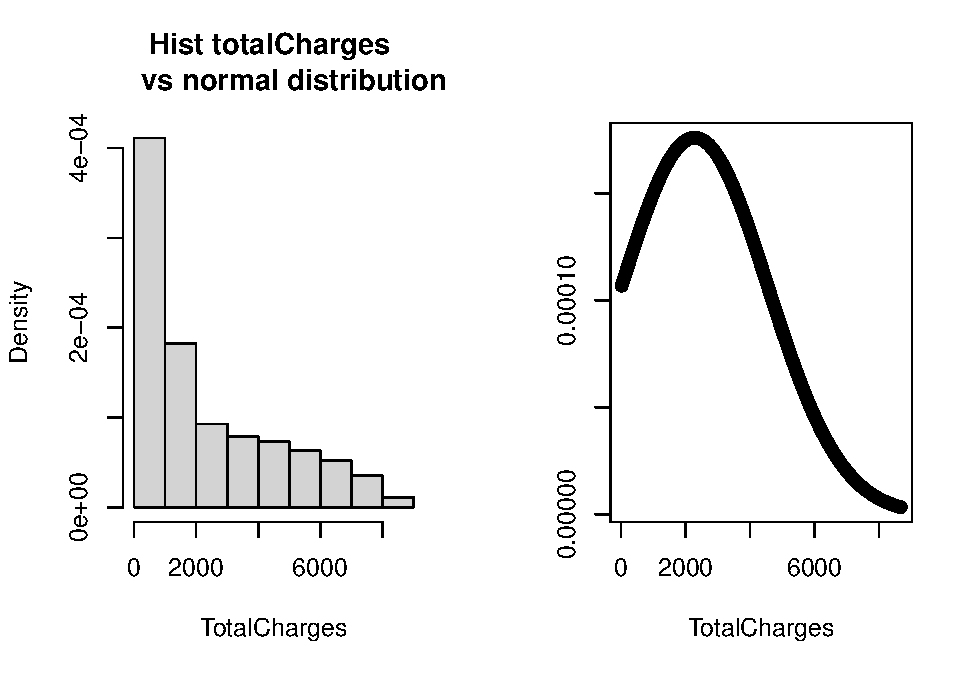
\includegraphics{AdriàCasanova-VíctorGarcia-ZhengyongJi_files/figure-latex/Analysis of normality-2.pdf}

\begin{Shaded}
\begin{Highlighting}[]
\FunctionTok{hist}\NormalTok{(df}\SpecialCharTok{$}\NormalTok{MonthlyCharges, }\AttributeTok{prob =} \ConstantTok{TRUE}\NormalTok{, }\AttributeTok{breaks =} \DecValTok{10}\NormalTok{, }\AttributeTok{main =} \StringTok{"Hist MonthlyCharges }
\StringTok{     vs normal distribution"}\NormalTok{,}
    \AttributeTok{xlab =} \StringTok{"df$MonthlyCharges"}\NormalTok{)}
\NormalTok{x }\OtherTok{\textless{}{-}} \FunctionTok{seq}\NormalTok{(}\FunctionTok{min}\NormalTok{(df}\SpecialCharTok{$}\NormalTok{MonthlyCharges, }\AttributeTok{na.rm =} \ConstantTok{TRUE}\NormalTok{), }\FunctionTok{max}\NormalTok{(df}\SpecialCharTok{$}\NormalTok{MonthlyCharges,}
    \AttributeTok{na.rm =} \ConstantTok{TRUE}\NormalTok{), }\AttributeTok{by =} \FloatTok{0.1}\NormalTok{)}
\NormalTok{y }\OtherTok{\textless{}{-}} \FunctionTok{dnorm}\NormalTok{(x, }\AttributeTok{mean =} \FunctionTok{mean}\NormalTok{(df}\SpecialCharTok{$}\NormalTok{MonthlyCharges, }\AttributeTok{na.rm =} \ConstantTok{TRUE}\NormalTok{), }\AttributeTok{sd =} \FunctionTok{sd}\NormalTok{(df}\SpecialCharTok{$}\NormalTok{MonthlyCharges,}
    \AttributeTok{na.rm =} \ConstantTok{TRUE}\NormalTok{))}
\FunctionTok{plot}\NormalTok{(x, y, }\AttributeTok{xlab =} \StringTok{"df$MonthlyCharges"}\NormalTok{, }\AttributeTok{ylab =} \StringTok{""}\NormalTok{)}
\end{Highlighting}
\end{Shaded}

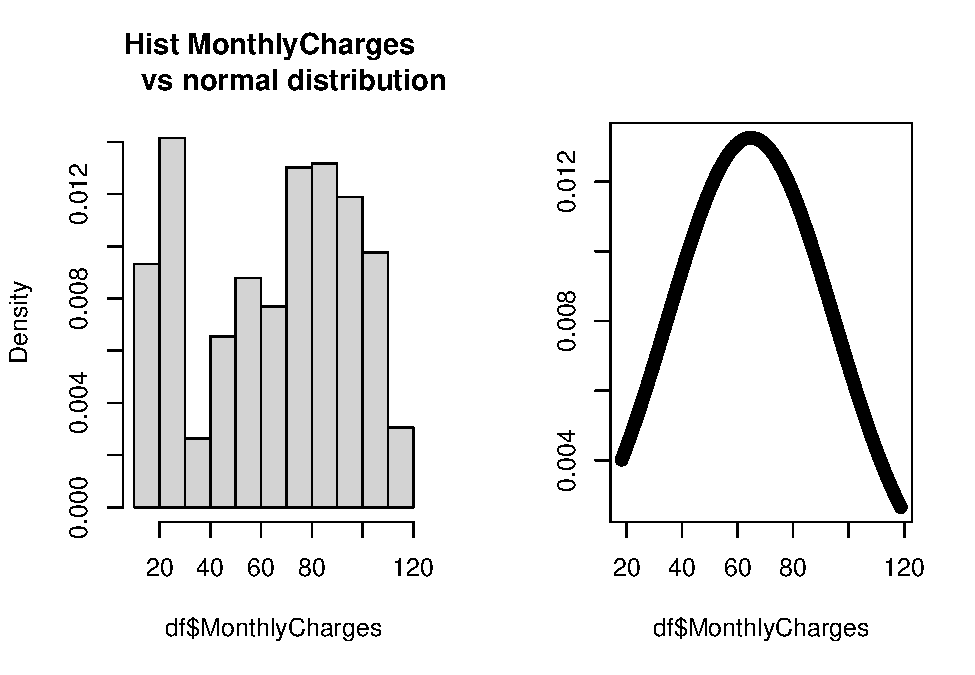
\includegraphics{AdriàCasanova-VíctorGarcia-ZhengyongJi_files/figure-latex/Analysis of normality-3.pdf}

\begin{Shaded}
\begin{Highlighting}[]
\FunctionTok{par}\NormalTok{(}\AttributeTok{mfrow =} \FunctionTok{c}\NormalTok{(}\DecValTok{1}\NormalTok{, }\DecValTok{1}\NormalTok{))}
\end{Highlighting}
\end{Shaded}

\hypertarget{data-quality-report}{%
\section{3. Data Quality Report}\label{data-quality-report}}

In this section we analysed the missing values, outliers and errors of
numeric variables to increase the quality of data before modeling.

To start with, we detected that only ``TotalCharges'', and hence
``c.TotalCharges'', has a total of 22 missing observations. However, all
of them correspond to new clients who have not receive their first
invoice yet, so ``TotalCharges'' can not have a value. In other words,
they are ``not applicable cases''. We naturally impute this observations
with 0.

\begin{Shaded}
\begin{Highlighting}[]
\CommentTok{\# Distribution of missings in df per variable}
\FunctionTok{apply}\NormalTok{(}\FunctionTok{sapply}\NormalTok{(df, is.na), }\DecValTok{2}\NormalTok{, sum)}
\end{Highlighting}
\end{Shaded}

\begin{verbatim}
##       customerID           gender    SeniorCitizen          Partner 
##                0                0                0                0 
##       Dependents           tenure     PhoneService    MultipleLines 
##                0                0                0                0 
##  InternetService   OnlineSecurity     OnlineBackup DeviceProtection 
##                0                0                0                0 
##      TechSupport      StreamingTV  StreamingMovies         Contract 
##                0                0                0                0 
## PaperlessBilling    PaymentMethod   MonthlyCharges     TotalCharges 
##                0                0                0               11 
##            Churn         c.tenure   c.TotalCharges c.MonthlyCharges 
##                0                0               11                0
\end{verbatim}

\begin{Shaded}
\begin{Highlighting}[]
\CommentTok{\# Distribution of missings in df per individual}
\FunctionTok{table}\NormalTok{(}\FunctionTok{apply}\NormalTok{(}\FunctionTok{sapply}\NormalTok{(df, is.na), }\DecValTok{1}\NormalTok{, sum))}
\end{Highlighting}
\end{Shaded}

\begin{verbatim}
## 
##    0    2 
## 7032   11
\end{verbatim}

\begin{Shaded}
\begin{Highlighting}[]
\CommentTok{\# Check that all missings in \textquotesingle{}TotalCharges\textquotesingle{} correspond to}
\CommentTok{\# individuals tenure = 0}
\NormalTok{TotalCharges.na }\OtherTok{\textless{}{-}} \FunctionTok{which}\NormalTok{(}\FunctionTok{is.na}\NormalTok{(df}\SpecialCharTok{$}\NormalTok{TotalCharges))}
\FunctionTok{sum}\NormalTok{(TotalCharges.na }\SpecialCharTok{==} \FunctionTok{which}\NormalTok{(df}\SpecialCharTok{$}\NormalTok{tenure }\SpecialCharTok{==} \DecValTok{0}\NormalTok{)) }\SpecialCharTok{==} \FunctionTok{length}\NormalTok{(TotalCharges.na)}
\end{Highlighting}
\end{Shaded}

\begin{verbatim}
## [1] TRUE
\end{verbatim}

\begin{Shaded}
\begin{Highlighting}[]
\CommentTok{\# So we transform them after creating a new numeric}
\CommentTok{\# variable with all the missings of the database}
\NormalTok{df}\SpecialCharTok{$}\NormalTok{n.na }\OtherTok{\textless{}{-}} \FunctionTok{apply}\NormalTok{(}\FunctionTok{sapply}\NormalTok{(df, is.na), }\DecValTok{1}\NormalTok{, sum)}

\NormalTok{df}\SpecialCharTok{$}\NormalTok{TotalCharges[TotalCharges.na] }\OtherTok{=} \DecValTok{0}
\NormalTok{df}\SpecialCharTok{$}\NormalTok{c.TotalCharges[TotalCharges.na] }\OtherTok{=} \StringTok{"({-}1,2171]"}
\end{Highlighting}
\end{Shaded}

Secondly, we detected data inconsistencies. For categorical values, we
checked the EDA automatic reports and the summaries to ensure that all
qualitative variables categories were meaningful and that there was not
any misspelling errors. We also checked that all values of numeric
variables were positive and reasonable.

Additionally, for ``TotalCharges'' we ensured that all the values were
correct by manually calculating the value and comparing it to the actual
total charge.

\begin{Shaded}
\begin{Highlighting}[]
\CommentTok{\# Expected total charges as the product of monthly charges}
\CommentTok{\# and tenure}
\NormalTok{expected\_total\_charges }\OtherTok{=}\NormalTok{ df}\SpecialCharTok{$}\NormalTok{MonthlyCharges }\SpecialCharTok{*}\NormalTok{ df}\SpecialCharTok{$}\NormalTok{tenure}

\CommentTok{\# Plot them against the actual total charges}
\FunctionTok{plot}\NormalTok{(expected\_total\_charges, df}\SpecialCharTok{$}\NormalTok{TotalCharges)}
\end{Highlighting}
\end{Shaded}

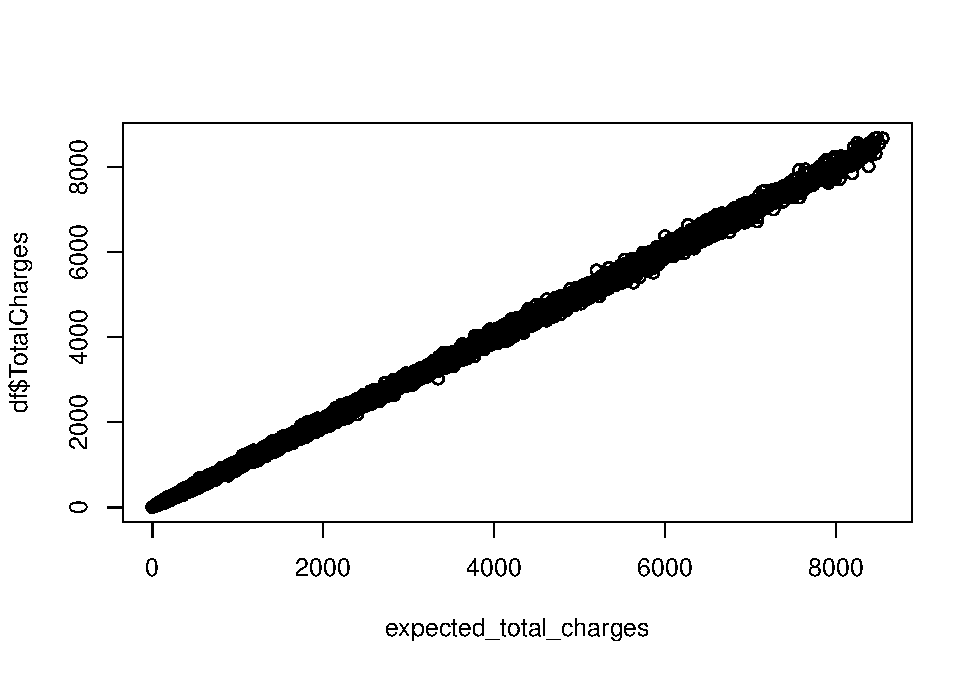
\includegraphics{AdriàCasanova-VíctorGarcia-ZhengyongJi_files/figure-latex/Compare TotalCharges to its expected values-1.pdf}

\begin{Shaded}
\begin{Highlighting}[]
\CommentTok{\# There are no outliers, so TotalCharges is consistent.}
\end{Highlighting}
\end{Shaded}

Thirdly, we analysed univariate outliers in numeric variables using
Boxplots and the typical thresholds: 1.5 * IQR(interquartile range) for
mild outliers and 3 * IQR for severe outliers. As there were not any we
considered that all points were suitable for our models.

\begin{Shaded}
\begin{Highlighting}[]
\FunctionTok{par}\NormalTok{(}\AttributeTok{mfrow =} \FunctionTok{c}\NormalTok{(}\DecValTok{1}\NormalTok{, }\FunctionTok{length}\NormalTok{(numeric\_val\_idx)))}
\ControlFlowTok{for}\NormalTok{ (var }\ControlFlowTok{in} \FunctionTok{as.numeric}\NormalTok{(numeric\_val\_idx)) \{}
    \FunctionTok{Boxplot}\NormalTok{(df[, var], }\AttributeTok{ylab =} \FunctionTok{names}\NormalTok{(df)[var], }\AttributeTok{main =} \StringTok{"Boxplot"}\NormalTok{)}
\NormalTok{\}}
\end{Highlighting}
\end{Shaded}

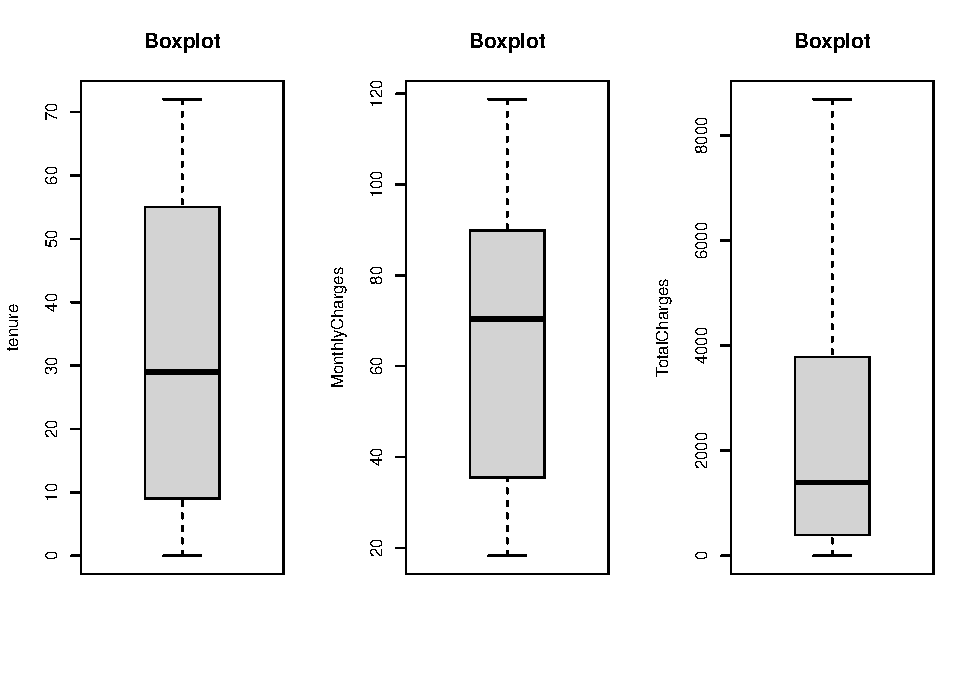
\includegraphics{AdriàCasanova-VíctorGarcia-ZhengyongJi_files/figure-latex/Boxplots-1.pdf}

\begin{Shaded}
\begin{Highlighting}[]
\FunctionTok{par}\NormalTok{(}\AttributeTok{mfrow =} \FunctionTok{c}\NormalTok{(}\DecValTok{1}\NormalTok{, }\DecValTok{1}\NormalTok{))}
\end{Highlighting}
\end{Shaded}

\hypertarget{in-depth-analysis-of-missing-values}{%
\subsection{3.1 In depth analysis of missing
values}\label{in-depth-analysis-of-missing-values}}

Next, we will compute for every group of individuals the mean of missing
values. Then we will rank the groups according to the computed mean.

\begin{Shaded}
\begin{Highlighting}[]
\CommentTok{\# c.TotalCharges has missings, so it doesn\textquotesingle{}t make sense to}
\CommentTok{\# compute the mean of missings in its categories}

\NormalTok{interesting\_cat\_idx }\OtherTok{\textless{}{-}}\NormalTok{ categoric\_val\_idx[}\SpecialCharTok{{-}}\FunctionTok{c}\NormalTok{(}\DecValTok{1}\NormalTok{, }\DecValTok{20}\NormalTok{)]}
\NormalTok{k }\OtherTok{=} \DecValTok{0}
\ControlFlowTok{for}\NormalTok{ (i }\ControlFlowTok{in}\NormalTok{ interesting\_cat\_idx) \{}
\NormalTok{    k }\OtherTok{\textless{}{-}}\NormalTok{ k }\SpecialCharTok{+} \FunctionTok{length}\NormalTok{(}\FunctionTok{levels}\NormalTok{(df[, i]))}
\NormalTok{\}}
\NormalTok{groups.na }\OtherTok{\textless{}{-}} \FunctionTok{matrix}\NormalTok{(}\DecValTok{0}\NormalTok{, k, }\DecValTok{2}\NormalTok{)}
\NormalTok{l }\OtherTok{=} \DecValTok{1}
\ControlFlowTok{for}\NormalTok{ (idx }\ControlFlowTok{in}\NormalTok{ interesting\_cat\_idx) \{}
\NormalTok{    categories.na }\OtherTok{\textless{}{-}} \FunctionTok{tapply}\NormalTok{(df}\SpecialCharTok{$}\NormalTok{n.na, df[, idx], mean)}
    \ControlFlowTok{for}\NormalTok{ (j }\ControlFlowTok{in} \FunctionTok{seq}\NormalTok{(}\FunctionTok{length}\NormalTok{(categories.na))) \{}
\NormalTok{        groups.na[l }\SpecialCharTok{+}\NormalTok{ j }\SpecialCharTok{{-}} \DecValTok{1}\NormalTok{, ] }\OtherTok{\textless{}{-}} \FunctionTok{c}\NormalTok{(categories.na[j], }\FunctionTok{paste}\NormalTok{(}\FunctionTok{names}\NormalTok{(df)[idx],}
            \FunctionTok{levels}\NormalTok{(df[, idx])[j], }\AttributeTok{sep =} \StringTok{"."}\NormalTok{))}
\NormalTok{    \}}
\NormalTok{    l }\OtherTok{\textless{}{-}}\NormalTok{ l }\SpecialCharTok{+}\NormalTok{ j}
\NormalTok{\}}
\NormalTok{groups.na.df }\OtherTok{\textless{}{-}} \FunctionTok{data.frame}\NormalTok{(}\AttributeTok{na.perc =}\NormalTok{ groups.na[, }\DecValTok{1}\NormalTok{], }\AttributeTok{group =}\NormalTok{ groups.na[,}
    \DecValTok{2}\NormalTok{])}
\NormalTok{groups.na.df[}\FunctionTok{order}\NormalTok{(groups.na.df}\SpecialCharTok{$}\NormalTok{na.perc, }\AttributeTok{decreasing =} \ConstantTok{TRUE}\NormalTok{),}
\NormalTok{    ]}
\end{Highlighting}
\end{Shaded}

\begin{verbatim}
##                 na.perc                                   group
## 37   0.0117994100294985                       Contract.Two year
## 8    0.0104265402843602                          Dependents.Yes
## 43  0.00992555831265509              PaymentMethod.Mailed check
## 46  0.00804681784930505                        c.tenure.(-1,18]
## 16  0.00786369593709043                      InternetService.No
## 18  0.00786369593709043      OnlineSecurity.No internet service
## 21  0.00786369593709043        OnlineBackup.No internet service
## 24  0.00786369593709043    DeviceProtection.No internet service
## 27  0.00786369593709043         TechSupport.No internet service
## 30  0.00786369593709043         StreamingTV.No internet service
## 33  0.00786369593709043     StreamingMovies.No internet service
## 50  0.00734394124847001             c.MonthlyCharges.(18,30.69]
## 9   0.00586510263929619                         PhoneService.No
## 12  0.00586510263929619          MultipleLines.No phone service
## 38  0.00557103064066852                     PaperlessBilling.No
## 6   0.00529100529100529                             Partner.Yes
## 44  0.00425202937765752                                Churn.No
## 14  0.00413052457662123                     InternetService.DSL
## 19  0.00396235760277365                      OnlineSecurity.Yes
## 28  0.00391389432485323                         TechSupport.Yes
## 3   0.00372818166412472                       SeniorCitizen.Yes
## 2   0.00337552742616034                             gender.Male
## 51   0.0033112582781457          c.MonthlyCharges.(30.69,59.38]
## 25  0.00330305532617671                    DeviceProtection.Yes
## 22  0.00329353643474681                        OnlineBackup.Yes
## 31  0.00295530107129664                         StreamingTV.Yes
## 11  0.00294985250737463                        MultipleLines.No
## 32  0.00287253141831239                      StreamingMovies.No
## 1   0.00286697247706422                           gender.Female
## 10  0.00282974375098255                        PhoneService.Yes
## 13  0.00269269606193201                       MultipleLines.Yes
## 40  0.00259067357512953 PaymentMethod.Bank transfer (automatic)
## 52  0.00258955545964609          c.MonthlyCharges.(59.38,89.06]
## 39  0.00143850395588588                    PaperlessBilling.Yes
## 36  0.00135777325186694                       Contract.One year
## 41  0.00131406044678055   PaymentMethod.Credit card (automatic)
## 5   0.00109859928591046                              Partner.No
## 34 0.000732064421669107                     StreamingMovies.Yes
## 29 0.000711743772241993                          StreamingTV.No
## 20 0.000647668393782383                         OnlineBackup.No
## 23 0.000646203554119548                     DeviceProtection.No
## 26 0.000575871004894904                          TechSupport.No
## 17 0.000571755288736421                       OnlineSecurity.No
## 4                     0                        SeniorCitizen.No
## 7                     0                           Dependents.No
## 15                    0             InternetService.Fiber optic
## 35                    0                 Contract.Month-to-month
## 42                    0          PaymentMethod.Electronic check
## 45                    0                               Churn.Yes
## 47                    0                        c.tenure.(18,36]
## 48                    0                        c.tenure.(36,54]
## 49                    0                        c.tenure.(54,72]
## 53                    0         c.MonthlyCharges.(89.06,118.75]
\end{verbatim}

The groups with the highest proportion of missing data are made of those
individuals who:

\begin{itemize}
\tightlist
\item
  Have a two-year contract
\item
  Have dependents
\item
  Pay with a mailed check
\end{itemize}

Since the set of individuals with missing data is exactly that of the
new clients, we conclude that recently incorporated clients tend to:
sign a two-year contract, have dependents and pay with a mailed check.

We can compute as well the pearson correlation coefficient between
``n.na'' and the numerical variables.

\begin{Shaded}
\begin{Highlighting}[]
\CommentTok{\# Creation of the correlation matrix}
\NormalTok{corr\_mat }\OtherTok{\textless{}{-}} \FunctionTok{cor}\NormalTok{(df[, }\FunctionTok{c}\NormalTok{(numeric\_val\_idx, }\DecValTok{25}\NormalTok{)], )}
\NormalTok{corr\_mat}
\end{Highlighting}
\end{Shaded}

\begin{verbatim}
##                     tenure MonthlyCharges TotalCharges        n.na
## tenure          1.00000000     0.24789986   0.82617840 -0.05213467
## MonthlyCharges  0.24789986     1.00000000   0.65117383 -0.03068535
## TotalCharges    0.82617840     0.65117383   1.00000000 -0.03977955
## n.na           -0.05213467    -0.03068535  -0.03977955  1.00000000
\end{verbatim}

\begin{Shaded}
\begin{Highlighting}[]
\FunctionTok{corrplot}\NormalTok{(corr\_mat, }\AttributeTok{order =} \StringTok{"hclust"}\NormalTok{, }\AttributeTok{tl.cex =} \FloatTok{0.9}\NormalTok{)}
\end{Highlighting}
\end{Shaded}

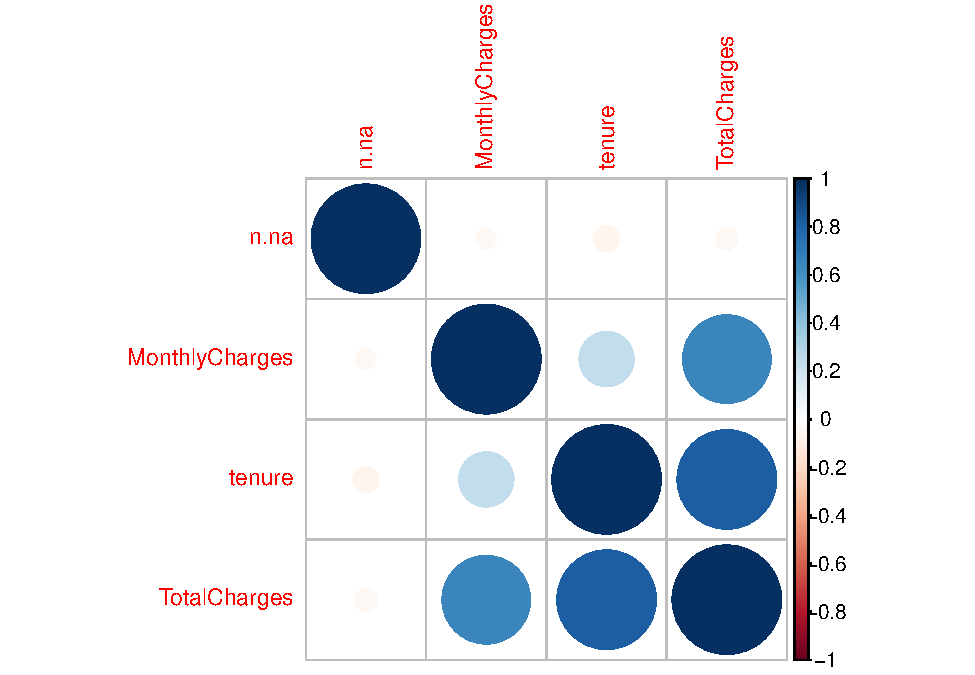
\includegraphics{AdriàCasanova-VíctorGarcia-ZhengyongJi_files/figure-latex/n.na correlations-1.pdf}

n.na is independent to the rest of numerical variables, probably because
it evaluates to 0 in most observations.

\hypertarget{multivariate-outliers}{%
\subsection{3.2 Multivariate outliers}\label{multivariate-outliers}}

In this section we focused on detecting the multivariate outliers using
``Moutlier''. We discovered 344 multivariate outliers, about 5\% of the
individuals, as it was expected. We decided to maintain them and only
remove them in the modeling step if they turned out to be influential
points.

\begin{Shaded}
\begin{Highlighting}[]
\FunctionTok{set.seed}\NormalTok{(}\DecValTok{123}\NormalTok{)}
\NormalTok{res.mout }\OtherTok{\textless{}{-}} \FunctionTok{Moutlier}\NormalTok{(df[, numeric\_val\_idx], }\AttributeTok{quantile =} \FloatTok{0.95}\NormalTok{,}
    \AttributeTok{plot =} \ConstantTok{FALSE}\NormalTok{)}

\CommentTok{\# Visual representation}
\FunctionTok{par}\NormalTok{(}\AttributeTok{mfrow =} \FunctionTok{c}\NormalTok{(}\DecValTok{1}\NormalTok{, }\DecValTok{2}\NormalTok{), }\AttributeTok{cex.main =} \FloatTok{0.8}\NormalTok{)}
\FunctionTok{plot}\NormalTok{(res.mout}\SpecialCharTok{$}\NormalTok{md, }\AttributeTok{col =} \StringTok{"lightblue"}\NormalTok{, }\AttributeTok{pch =} \DecValTok{19}\NormalTok{, }\AttributeTok{main =} \StringTok{"Detection of multivariable }
\StringTok{outliers"}\NormalTok{,}
    \AttributeTok{xlab =} \StringTok{"Observation"}\NormalTok{, }\AttributeTok{ylab =} \StringTok{"Traditional Mahalanobis distance "}\NormalTok{)}
\FunctionTok{abline}\NormalTok{(}\AttributeTok{h =}\NormalTok{ res.mout}\SpecialCharTok{$}\NormalTok{cutoff, }\AttributeTok{col =} \StringTok{"red"}\NormalTok{, }\AttributeTok{lwd =} \DecValTok{5}\NormalTok{, }\AttributeTok{lty =} \DecValTok{2}\NormalTok{)}

\FunctionTok{plot}\NormalTok{(res.mout}\SpecialCharTok{$}\NormalTok{rd, }\AttributeTok{col =} \StringTok{"lightblue"}\NormalTok{, }\AttributeTok{pch =} \DecValTok{19}\NormalTok{, }\AttributeTok{xlab =} \StringTok{"Observation"}\NormalTok{,}
    \AttributeTok{ylab =} \StringTok{"Robust Mahalanobis distance "}\NormalTok{)}
\FunctionTok{abline}\NormalTok{(}\AttributeTok{h =}\NormalTok{ res.mout}\SpecialCharTok{$}\NormalTok{cutoff, }\AttributeTok{col =} \StringTok{"red"}\NormalTok{, }\AttributeTok{lwd =} \DecValTok{5}\NormalTok{, }\AttributeTok{lty =} \DecValTok{2}\NormalTok{)}
\end{Highlighting}
\end{Shaded}

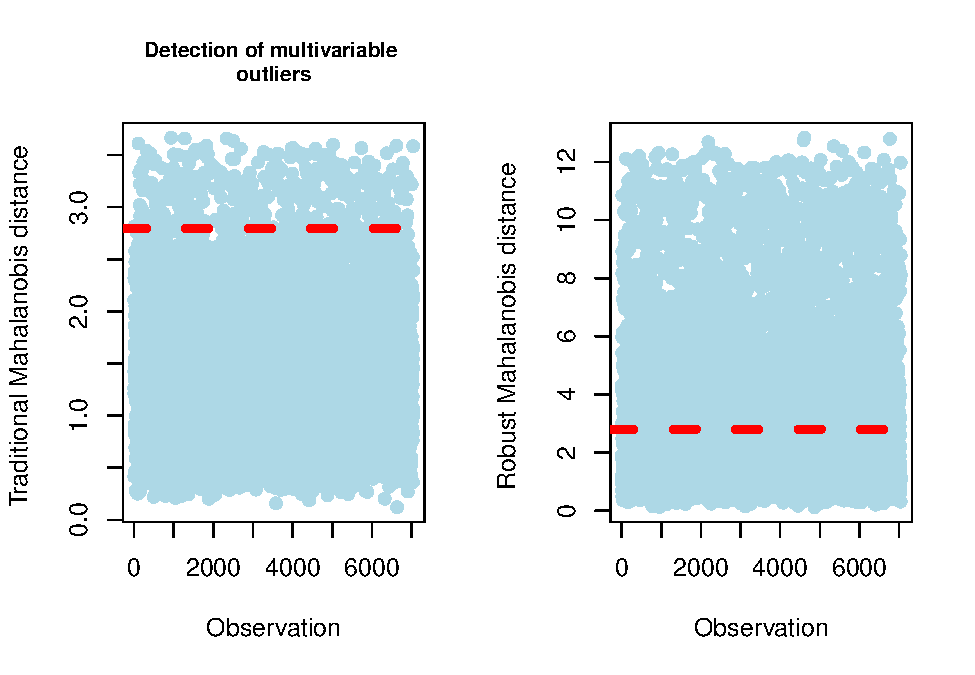
\includegraphics{AdriàCasanova-VíctorGarcia-ZhengyongJi_files/figure-latex/Moutlier-1.pdf}

\begin{Shaded}
\begin{Highlighting}[]
\FunctionTok{par}\NormalTok{(}\AttributeTok{mfrow =} \FunctionTok{c}\NormalTok{(}\DecValTok{1}\NormalTok{, }\DecValTok{1}\NormalTok{), }\AttributeTok{cex.main =} \DecValTok{1}\NormalTok{)}

\CommentTok{\# Identification of the outliers}
\NormalTok{outliers }\OtherTok{=} \FunctionTok{which}\NormalTok{(res.mout}\SpecialCharTok{$}\NormalTok{md }\SpecialCharTok{\textgreater{}}\NormalTok{ res.mout}\SpecialCharTok{$}\NormalTok{cutoff }\SpecialCharTok{\&}\NormalTok{ res.mout}\SpecialCharTok{$}\NormalTok{rd }\SpecialCharTok{\textgreater{}}
\NormalTok{    res.mout}\SpecialCharTok{$}\NormalTok{cutoff)}
\FunctionTok{length}\NormalTok{(outliers)}
\end{Highlighting}
\end{Shaded}

\begin{verbatim}
## [1] 344
\end{verbatim}

\begin{Shaded}
\begin{Highlighting}[]
\FunctionTok{length}\NormalTok{(outliers)}\SpecialCharTok{/}\FunctionTok{dim}\NormalTok{(df)[}\DecValTok{1}\NormalTok{] }\SpecialCharTok{*} \DecValTok{100}
\end{Highlighting}
\end{Shaded}

\begin{verbatim}
## [1] 4.884282
\end{verbatim}

\hypertarget{profiling-of-the-target-and-feature-selection}{%
\section{4. Profiling of the target and feature
selection}\label{profiling-of-the-target-and-feature-selection}}

\hypertarget{numeric-variables-correlations}{%
\subsection{Numeric variables'
correlations}\label{numeric-variables-correlations}}

We analysed the pearson correlation coefficient to detect variables that
were highly related and not include them all in the model. In the
correlation plot of section 3.1 we see that ``TotalCharges'' is highly
correlated with ``MonthlyCharges'' and ``tenure'' as the first one is
calculated as the product of the others.

\hypertarget{profiling-of-the-target}{%
\subsection{Profiling of the target}\label{profiling-of-the-target}}

Later on, we profiled the target Churn using a custom function
``profiling()'' created in the Multivariate Analysis subject of the
Master's degree. This method expands ``catdes()'' and performs many
plots and tests according to the type of each variable. We will focus on
plots and the given tests' results: Chi\^{}2, ANOVA and Kruskal-Wallis,
which can be found in the annex.

\begin{Shaded}
\begin{Highlighting}[]
\CommentTok{\# Analysis of all variables except the ID}
\FunctionTok{profiling}\NormalTok{(df[}\SpecialCharTok{{-}}\FunctionTok{c}\NormalTok{(}\FunctionTok{grep}\NormalTok{(}\StringTok{"customerID"}\NormalTok{, }\FunctionTok{names}\NormalTok{(df)), }\FunctionTok{grep}\NormalTok{(}\StringTok{"Churn"}\NormalTok{,}
    \FunctionTok{names}\NormalTok{(df)))], df}\SpecialCharTok{$}\NormalTok{Churn, }\StringTok{"Churn"}\NormalTok{)}
\end{Highlighting}
\end{Shaded}

The most relevant conclusions are: - Some variables are not significant,
like Gender (Chi\^{}2 p-value=0.4866) or Phone service (Chi\^{}2
p-value=0.3388). Consequently, we state that churn is independent of the
client's gender and whether he/she/they has a phone service contracted.

\begin{Shaded}
\begin{Highlighting}[]
\FunctionTok{profiling}\NormalTok{(df[}\FunctionTok{c}\NormalTok{(}\FunctionTok{grep}\NormalTok{(}\StringTok{"gender"}\NormalTok{, }\FunctionTok{names}\NormalTok{(df)), }\FunctionTok{grep}\NormalTok{(}\StringTok{"PhoneService"}\NormalTok{,}
    \FunctionTok{names}\NormalTok{(df)))], df}\SpecialCharTok{$}\NormalTok{Churn, }\StringTok{"Churn"}\NormalTok{)}
\end{Highlighting}
\end{Shaded}

\begin{itemize}
\tightlist
\item
  There are variables like ``MultipleLines'' that even being significant
  (Chi\^{}2 p-value=0.003464) the difference among levels is small, as
  we can see in the plots
\end{itemize}

\begin{Shaded}
\begin{Highlighting}[]
\FunctionTok{profiling}\NormalTok{(df[}\FunctionTok{grep}\NormalTok{(}\StringTok{"MultipleLines"}\NormalTok{, }\FunctionTok{names}\NormalTok{(df))], df}\SpecialCharTok{$}\NormalTok{Churn, }\StringTok{"Churn"}\NormalTok{)}
\end{Highlighting}
\end{Shaded}

\begin{itemize}
\tightlist
\item
  The rest of variables, including the discretized, have a small p-value
  (\textless{} 2.2e-16) in the Chi\^{}2, ANOVA or Kruskal-Wallis test,
  according to their type, and have at least one level where the
  target's distribution is different than in the rest. For example, 40\%
  of people that did not have an online backup churned, while only 22\%
  of customers having the backup did.
\end{itemize}

\begin{Shaded}
\begin{Highlighting}[]
\FunctionTok{profiling}\NormalTok{(df[}\FunctionTok{grep}\NormalTok{(}\StringTok{"OnlineBackup"}\NormalTok{, }\FunctionTok{names}\NormalTok{(df))], df}\SpecialCharTok{$}\NormalTok{Churn, }\StringTok{"Churn"}\NormalTok{)}
\end{Highlighting}
\end{Shaded}

\hypertarget{feature-selection}{%
\subsection{Feature Selection}\label{feature-selection}}

Finally, we decided which variables were suitable to be included in the
model.

The id was removed, since it will not give us any knowledge nor be
useful to predict the target.

\begin{Shaded}
\begin{Highlighting}[]
\NormalTok{df}\SpecialCharTok{$}\NormalTok{customerID }\OtherTok{\textless{}{-}} \ConstantTok{NULL}
\end{Highlighting}
\end{Shaded}

We then computed the relationship between all the variables and the
target with the ``catdes()'' method and chose the most relevant of them
for the target's explanation.

All p-values of the Chi-squared test for categorical variables are very
low, less than 0.001. The 6 variables with the lowest p-value are
Contract, OnlineSecurity, TechSupport, c.tenure, InternetService,
PaymentMethod. Note that the list includes a discretized numerical
variable.

\begin{Shaded}
\begin{Highlighting}[]
\CommentTok{\# Correlation between all variables and our qualitative}
\CommentTok{\# target Churn.}
\NormalTok{res.cat }\OtherTok{=} \FunctionTok{catdes}\NormalTok{(df, }\FunctionTok{grep}\NormalTok{(}\StringTok{"Churn"}\NormalTok{, }\FunctionTok{names}\NormalTok{(df)))}

\CommentTok{\# Most important categorical variables, sorted by p value}
\NormalTok{res.cat}\SpecialCharTok{$}\NormalTok{test.chi2}
\end{Highlighting}
\end{Shaded}

\begin{verbatim}
##                        p.value df
## Contract         5.863038e-258  2
## OnlineSecurity   2.661150e-185  2
## TechSupport      1.443084e-180  2
## c.tenure         4.192004e-178  3
## InternetService  9.571788e-160  2
## PaymentMethod    3.682355e-140  3
## OnlineBackup     2.079759e-131  2
## DeviceProtection 5.505219e-122  2
## StreamingMovies   2.667757e-82  2
## StreamingTV       5.528994e-82  2
## c.MonthlyCharges  8.977393e-72  3
## PaperlessBilling  2.614597e-58  1
## Dependents        3.276083e-43  1
## c.TotalCharges    3.057813e-39  3
## SeniorCitizen     9.477904e-37  1
## Partner           1.519037e-36  1
## MultipleLines     3.464383e-03  2
\end{verbatim}

As for numeric variables, ``tenure'' has the smallest p-value in the
F-test, much lower than those of discrete variables. As we have already
seen, there is a high correlation between ``MonthlyCharges'', ``tenure''
and ``TotalCharges'' so we will only include in the models
``TotalCharges'' or ``MonthlyCharges'' together with ``tenure''.

\begin{Shaded}
\begin{Highlighting}[]
\NormalTok{res.cat}\SpecialCharTok{$}\NormalTok{quanti.var}
\end{Highlighting}
\end{Shaded}

\begin{verbatim}
##                      Eta2       P-value
## tenure         0.12406504 7.999058e-205
## TotalCharges   0.03933251  2.127212e-63
## MonthlyCharges 0.03738671  2.706646e-60
\end{verbatim}

\hypertarget{profiling-of-the-target-with-the-selected-categorical-features}{%
\subsection{Profiling of the target with the selected categorical
features}\label{profiling-of-the-target-with-the-selected-categorical-features}}

Lastly, we decided to make an extensive profiling of the six categorical
variables that we could use in the model in order to understand them
better. The main conclusions for each variable were:

\begin{itemize}
\item
  Contract: The probability of churning is decreased when the contract
  term increases. For example, if a costumer has a month contract and
  changes it to an annual the probability of not churning increases from
  0.58 to 0.89.
\item
  InternetService: People that do not have an internet service do not
  usually churn (7\%). However, if they had a Fiber optic connection,
  the probability to churn increases (42\%). This could be explained by
  the fact that users with a fast internet connection try to get the
  best offer for the service, but it would be necessary to make a market
  analysis to validate this hypothesis.
\item
  OnlineSecurity: The probability of churning is small when the customer
  has online security. However, having an internet connection or not
  seems a more interesting feature than the variable itself, as the ``No
  internet service'' level has the smallest p-value.
\item
  TechSupport: Having tech support increases the probability of not
  churning from 60\% to 84\% (when compared with not having it, although
  having internet service). Having internet service or not is, again, a
  more relevant feature.
\item
  c.tenure: Loyalty is important, since people tend to churn less when
  they have spent longer with the service. For example, people who have
  spent less than 1.5 years has churned 44\% of times, but only 8\% of
  those who have stayed for more than 4.5 years have churned.
\item
  PaymentMethod: The proportion of people that churned is very similar
  in all types of payment except for ``Electronic check''. In this
  level, the proportion of churns is 45\%, 18\% higher than the global
  average.
\end{itemize}

\begin{Shaded}
\begin{Highlighting}[]
\CommentTok{\# Global proportions of Churn categories}
\FunctionTok{proportions}\NormalTok{(}\FunctionTok{table}\NormalTok{(df}\SpecialCharTok{$}\NormalTok{Churn))}
\end{Highlighting}
\end{Shaded}

\begin{verbatim}
## 
##        No       Yes 
## 0.7346301 0.2653699
\end{verbatim}

\begin{Shaded}
\begin{Highlighting}[]
\CommentTok{\# Calculate the indexes of the variables to investigate}
\NormalTok{names }\OtherTok{=} \FunctionTok{c}\NormalTok{(}\StringTok{"Contract"}\NormalTok{, }\StringTok{"OnlineSecurity"}\NormalTok{, }\StringTok{"TechSupport"}\NormalTok{, }\StringTok{"c.tenure"}\NormalTok{,}
    \StringTok{"InternetService"}\NormalTok{, }\StringTok{"PaymentMethod"}\NormalTok{)}
\NormalTok{index }\OtherTok{=} \ConstantTok{NULL}

\ControlFlowTok{for}\NormalTok{ (i }\ControlFlowTok{in} \DecValTok{1}\SpecialCharTok{:}\FunctionTok{length}\NormalTok{(names)) \{}
\NormalTok{    ind }\OtherTok{=} \FunctionTok{grep}\NormalTok{(names[i], }\FunctionTok{colnames}\NormalTok{(df))}
\NormalTok{    index }\OtherTok{=} \FunctionTok{append}\NormalTok{(index, ind)}
\NormalTok{\}}
\NormalTok{index }\OtherTok{=} \FunctionTok{append}\NormalTok{(index, }\FunctionTok{grep}\NormalTok{(}\StringTok{"Churn"}\NormalTok{, }\FunctionTok{names}\NormalTok{(df)))}

\CommentTok{\# Profiling of only those variables}
\NormalTok{res.cat2 }\OtherTok{=} \FunctionTok{catdes}\NormalTok{(df[, index], }\FunctionTok{length}\NormalTok{(index))}

\NormalTok{res.cat2}\SpecialCharTok{$}\NormalTok{category}
\end{Highlighting}
\end{Shaded}

\begin{verbatim}
## $No
##                                          Cla/Mod  Mod/Cla   Global
## Contract=Two year                       97.16814 31.83224 24.06645
## c.tenure=(54,72]                        92.02859 32.35408 25.82706
## InternetService=No                      92.59502 27.30963 21.66690
## TechSupport=No internet service         92.59502 27.30963 21.66690
## OnlineSecurity=No internet service      92.59502 27.30963 21.66690
## Contract=One year                       88.73048 25.26092 20.91438
## OnlineSecurity=Yes                      85.38881 33.32045 28.66676
## TechSupport=Yes                         84.83366 33.51372 29.02172
## PaymentMethod=Credit card (automatic)   84.75690 24.93235 21.61011
## InternetService=DSL                     81.04089 37.92037 34.37456
## PaymentMethod=Bank transfer (automatic) 83.29016 24.85504 21.92248
## PaymentMethod=Mailed check              80.89330 25.20294 22.88797
## c.tenure=(36,54]                        81.97970 18.72826 16.78262
## c.tenure=(18,36]                        77.29358 19.54001 18.57163
## PaymentMethod=Electronic check          54.71459 25.00966 33.57944
## InternetService=Fiber optic             58.10724 34.77000 43.95854
## c.tenure=(-1,18]                        55.59620 29.37766 38.81869
## TechSupport=No                          58.36453 39.17665 49.31137
## OnlineSecurity=No                       58.23328 39.36993 49.66634
## Contract=Month-to-month                 57.29032 42.90684 55.01917
##                                               p.value     v.test
## Contract=Two year                       3.588830e-187  29.178937
## c.tenure=(54,72]                        2.745248e-113  22.620153
## InternetService=No                       6.584621e-98  20.999812
## TechSupport=No internet service          6.584621e-98  20.999812
## OnlineSecurity=No internet service       6.584621e-98  20.999812
## Contract=One year                        3.593041e-57  15.935502
## OnlineSecurity=Yes                       1.606459e-50  14.947938
## TechSupport=Yes                          1.323174e-46  14.334963
## PaymentMethod=Credit card (automatic)    6.408166e-32  11.758206
## InternetService=DSL                      2.545367e-26  10.614727
## PaymentMethod=Bank transfer (automatic)  1.180908e-24  10.250207
## PaymentMethod=Mailed check               3.226893e-15   7.881803
## c.tenure=(36,54]                         6.217772e-14   7.503412
## c.tenure=(18,36]                         4.375264e-04   3.516348
## PaymentMethod=Electronic check          1.790860e-136 -24.864755
## InternetService=Fiber optic             2.289126e-148 -25.941138
## c.tenure=(-1,18]                        7.876341e-159 -26.852547
## TechSupport=No                          1.899538e-183 -28.883947
## OnlineSecurity=No                       6.171504e-190 -29.396034
## Contract=Month-to-month                 3.620915e-283 -35.959308
## 
## $Yes
##                                           Cla/Mod   Mod/Cla   Global
## Contract=Month-to-month                 42.709677 88.550027 55.01917
## OnlineSecurity=No                       41.766724 78.170144 49.66634
## TechSupport=No                          41.635474 77.367576 49.31137
## c.tenure=(-1,18]                        44.403804 64.954521 38.81869
## InternetService=Fiber optic             41.892765 69.395399 43.95854
## PaymentMethod=Electronic check          45.285412 57.303371 33.57944
## c.tenure=(18,36]                        22.706422 15.890851 18.57163
## c.tenure=(36,54]                        18.020305 11.396469 16.78262
## PaymentMethod=Mailed check              19.106700 16.479401 22.88797
## PaymentMethod=Bank transfer (automatic) 16.709845 13.804173 21.92248
## InternetService=DSL                     18.959108 24.558587 34.37456
## PaymentMethod=Credit card (automatic)   15.243101 12.413055 21.61011
## TechSupport=Yes                         15.166341 16.586410 29.02172
## OnlineSecurity=Yes                      14.611194 15.783842 28.66676
## Contract=One year                       11.269518  8.881755 20.91438
## InternetService=No                       7.404980  6.046014 21.66690
## TechSupport=No internet service          7.404980  6.046014 21.66690
## OnlineSecurity=No internet service       7.404980  6.046014 21.66690
## c.tenure=(54,72]                         7.971413  7.758159 25.82706
## Contract=Two year                        2.831858  2.568218 24.06645
##                                               p.value     v.test
## Contract=Month-to-month                 3.620915e-283  35.959308
## OnlineSecurity=No                       6.171504e-190  29.396034
## TechSupport=No                          1.899538e-183  28.883947
## c.tenure=(-1,18]                        7.876341e-159  26.852547
## InternetService=Fiber optic             2.289126e-148  25.941138
## PaymentMethod=Electronic check          1.790860e-136  24.864755
## c.tenure=(18,36]                         4.375264e-04  -3.516348
## c.tenure=(36,54]                         6.217772e-14  -7.503412
## PaymentMethod=Mailed check               3.226893e-15  -7.881803
## PaymentMethod=Bank transfer (automatic)  1.180908e-24 -10.250207
## InternetService=DSL                      2.545367e-26 -10.614727
## PaymentMethod=Credit card (automatic)    6.408166e-32 -11.758206
## TechSupport=Yes                          1.323174e-46 -14.334963
## OnlineSecurity=Yes                       1.606459e-50 -14.947938
## Contract=One year                        3.593041e-57 -15.935502
## InternetService=No                       6.584621e-98 -20.999812
## TechSupport=No internet service          6.584621e-98 -20.999812
## OnlineSecurity=No internet service       6.584621e-98 -20.999812
## c.tenure=(54,72]                        2.745248e-113 -22.620153
## Contract=Two year                       3.588830e-187 -29.178937
\end{verbatim}

\begin{Shaded}
\begin{Highlighting}[]
\CommentTok{\# Another visualization of the profiling}
\CommentTok{\# profiling(df[,index], df$Churn, \textquotesingle{}Churn\textquotesingle{})}
\end{Highlighting}
\end{Shaded}

\hypertarget{modeling}{%
\section{5. Modeling}\label{modeling}}

\hypertarget{data-splitting}{%
\subsection{Data splitting}\label{data-splitting}}

First, let's split the dataset into training and testing set. We have
decided that 70\% of the data will be used for training.

\begin{Shaded}
\begin{Highlighting}[]
\FunctionTok{set.seed}\NormalTok{(}\DecValTok{123}\NormalTok{)}

\NormalTok{sampling }\OtherTok{=} \FunctionTok{sample.split}\NormalTok{(df}\SpecialCharTok{$}\NormalTok{Churn, }\AttributeTok{SplitRatio =} \FloatTok{0.7}\NormalTok{)}
\NormalTok{train }\OtherTok{=} \FunctionTok{subset}\NormalTok{(df, sampling }\SpecialCharTok{==} \ConstantTok{TRUE}\NormalTok{)}
\NormalTok{test }\OtherTok{=} \FunctionTok{subset}\NormalTok{(df, sampling }\SpecialCharTok{==} \ConstantTok{FALSE}\NormalTok{)}
\end{Highlighting}
\end{Shaded}

\hypertarget{modeling-only-with-numerical-variables}{%
\subsection{Modeling only with numerical
variables}\label{modeling-only-with-numerical-variables}}

As we mentioned, there is a strong correlation between \{tenure,
MonthlyCharges\} and TotalCharges, as the second one is simply the
product of the variables in the first set. Hence, we will build two
models, one for each set of variables, and keep the best one.

\begin{Shaded}
\begin{Highlighting}[]
\NormalTok{m0.set1 }\OtherTok{=} \FunctionTok{glm}\NormalTok{(Churn }\SpecialCharTok{\textasciitilde{}}\NormalTok{ tenure }\SpecialCharTok{+}\NormalTok{ MonthlyCharges, }\AttributeTok{data =}\NormalTok{ train,}
    \AttributeTok{family =}\NormalTok{ binomial)}
\CommentTok{\# Checking the Anova test, both variables are significant}
\CommentTok{\# to our model. Hence, we won\textquotesingle{}t remove any of them.}
\FunctionTok{Anova}\NormalTok{(m0.set1, }\AttributeTok{test =} \StringTok{"LR"}\NormalTok{)}
\end{Highlighting}
\end{Shaded}

\begin{verbatim}
## Analysis of Deviance Table (Type II tests)
## 
## Response: Churn
##                LR Chisq Df Pr(>Chisq)    
## tenure          1071.50  1  < 2.2e-16 ***
## MonthlyCharges   583.55  1  < 2.2e-16 ***
## ---
## Signif. codes:  0 '***' 0.001 '**' 0.01 '*' 0.05 '.' 0.1 ' ' 1
\end{verbatim}

\begin{Shaded}
\begin{Highlighting}[]
\NormalTok{m0.set2 }\OtherTok{=} \FunctionTok{glm}\NormalTok{(Churn }\SpecialCharTok{\textasciitilde{}}\NormalTok{ TotalCharges, }\AttributeTok{data =}\NormalTok{ train, }\AttributeTok{family =}\NormalTok{ binomial)}

\FunctionTok{BIC}\NormalTok{(m0.set1, m0.set2)}
\end{Highlighting}
\end{Shaded}

\begin{verbatim}
##         df      BIC
## m0.set1  3 4444.286
## m0.set2  2 5504.792
\end{verbatim}

Checking the Bayesian criterion, the set \{tenure, MonthlyCharges\} has
a much lower value and its variables are significant. Hence, we'll
choose this set of variables for further analysis.

We also check possible transformation for our model m0.set1.

\begin{Shaded}
\begin{Highlighting}[]
\NormalTok{m0.log }\OtherTok{=} \FunctionTok{glm}\NormalTok{(Churn }\SpecialCharTok{\textasciitilde{}}\NormalTok{ tenure }\SpecialCharTok{+} \FunctionTok{log}\NormalTok{(MonthlyCharges), }\AttributeTok{data =}\NormalTok{ train,}
    \AttributeTok{family =}\NormalTok{ binomial)}
\NormalTok{m0.sqrt }\OtherTok{=} \FunctionTok{glm}\NormalTok{(Churn }\SpecialCharTok{\textasciitilde{}} \FunctionTok{sqrt}\NormalTok{(tenure) }\SpecialCharTok{+}\NormalTok{ MonthlyCharges, }\AttributeTok{data =}\NormalTok{ train,}
    \AttributeTok{family =}\NormalTok{ binomial)}

\FunctionTok{BIC}\NormalTok{(m0.set1, m0.log, m0.sqrt)}
\end{Highlighting}
\end{Shaded}

\begin{verbatim}
##         df      BIC
## m0.set1  3 4444.286
## m0.log   3 4465.685
## m0.sqrt  3 4397.700
\end{verbatim}

We have tried several transformations for both variables (sqrt, log,
exp, etc), but BIC shows that the best model is the one with sqrt on
tenure.

Discretized variables might create a better model, so we study this
possibility.

\begin{Shaded}
\begin{Highlighting}[]
\NormalTok{m1 }\OtherTok{=} \FunctionTok{glm}\NormalTok{(Churn }\SpecialCharTok{\textasciitilde{}}\NormalTok{ c.tenure }\SpecialCharTok{+}\NormalTok{ MonthlyCharges, }\AttributeTok{data =}\NormalTok{ train, }\AttributeTok{family =}\NormalTok{ binomial)}

\FunctionTok{BIC}\NormalTok{(m1, m0.sqrt)}
\end{Highlighting}
\end{Shaded}

\begin{verbatim}
##         df      BIC
## m1       5 4585.287
## m0.sqrt  3 4397.700
\end{verbatim}

Checking the AIC and BIC parameters, we decided to keep the numerical
version of tenure. We have checked as well the model with MonthlyCharges
discretized, but the AIC is worse once more.

\hypertarget{residual-analysis-only-with-numerical-variables}{%
\subsection{Residual analysis only with numerical
variables}\label{residual-analysis-only-with-numerical-variables}}

It is important to look for influential points in the model that could
worsen it. ``influencePlot()'' computes the Cook's distance of each
point, so that we can compare them with the threshold studied in the
course.

\begin{Shaded}
\begin{Highlighting}[]
\CommentTok{\# Check influential points}
\NormalTok{influent }\OtherTok{=} \FunctionTok{influencePlot}\NormalTok{(m0.sqrt)[}\DecValTok{3}\NormalTok{]}
\end{Highlighting}
\end{Shaded}

\begin{Shaded}
\begin{Highlighting}[]
\NormalTok{influent}
\end{Highlighting}
\end{Shaded}

\begin{verbatim}
##             CookD
## 269  0.0059784386
## 431  0.0061523136
## 3827 0.0005332286
## 4381 0.0004744407
\end{verbatim}

\begin{Shaded}
\begin{Highlighting}[]
\CommentTok{\# Calculate D\textquotesingle{}s threshold}
\NormalTok{D\_thresh }\OtherTok{\textless{}{-}} \DecValTok{2}\SpecialCharTok{/}\FunctionTok{sqrt}\NormalTok{(}\FunctionTok{dim}\NormalTok{(train)[}\DecValTok{1}\NormalTok{])}
\NormalTok{D\_thresh}
\end{Highlighting}
\end{Shaded}

\begin{verbatim}
## [1] 0.02848436
\end{verbatim}

The Cook's distances obtained from ``influencePlot()'' are smaller than
our threshold, so we will not remove any point.

\hypertarget{adding-factor-main-effects-to-the-model}{%
\subsection{Adding factor main effects to the
model}\label{adding-factor-main-effects-to-the-model}}

After being satisfied with our final model based on numerical variables,
we add categorical variables to it in decreasing relevance order.

\begin{Shaded}
\begin{Highlighting}[]
\NormalTok{m2 }\OtherTok{=} \FunctionTok{glm}\NormalTok{(Churn }\SpecialCharTok{\textasciitilde{}} \FunctionTok{sqrt}\NormalTok{(tenure) }\SpecialCharTok{+}\NormalTok{ MonthlyCharges }\SpecialCharTok{+}\NormalTok{ Contract, }\AttributeTok{data =}\NormalTok{ train,}
    \AttributeTok{family =}\NormalTok{ binomial)}

\CommentTok{\# Adding \{contract\} indeed reduces the BIC of our model.}
\FunctionTok{BIC}\NormalTok{(m0.sqrt, m2)}
\end{Highlighting}
\end{Shaded}

\begin{verbatim}
##         df      BIC
## m0.sqrt  3 4397.700
## m2       5 4217.893
\end{verbatim}

\begin{Shaded}
\begin{Highlighting}[]
\NormalTok{m3 }\OtherTok{=} \FunctionTok{glm}\NormalTok{(Churn }\SpecialCharTok{\textasciitilde{}} \FunctionTok{sqrt}\NormalTok{(tenure) }\SpecialCharTok{+}\NormalTok{ MonthlyCharges }\SpecialCharTok{+}\NormalTok{ Contract }\SpecialCharTok{+}\NormalTok{ InternetService,}
    \AttributeTok{data =}\NormalTok{ train, }\AttributeTok{family =}\NormalTok{ binomial)}

\CommentTok{\# Adding \{InternetService\} indeed reduces the BIC of our}
\CommentTok{\# model.}
\FunctionTok{BIC}\NormalTok{(m2, m3)}
\end{Highlighting}
\end{Shaded}

\begin{verbatim}
##    df      BIC
## m2  5 4217.893
## m3  7 4190.321
\end{verbatim}

We have figured out in the profiling section that \{InternetService\}
and \{OnlineSecurity, TechSupport\} have some levels that are strongly
correlated. Specifically, when ``InternetService'' = ``No'',
``OnlineSecurity and''TechSupport'' can't be given a value, so they are
declared as ``No intervet service''.

To avoid multicollinearity and NA's, we need to decide which variable to
keep.

\begin{Shaded}
\begin{Highlighting}[]
\NormalTok{m4 }\OtherTok{=} \FunctionTok{glm}\NormalTok{(Churn }\SpecialCharTok{\textasciitilde{}} \FunctionTok{sqrt}\NormalTok{(tenure) }\SpecialCharTok{+}\NormalTok{ MonthlyCharges }\SpecialCharTok{+}\NormalTok{ Contract }\SpecialCharTok{+}\NormalTok{ OnlineSecurity }\SpecialCharTok{+}
\NormalTok{    TechSupport, }\AttributeTok{data =}\NormalTok{ train, }\AttributeTok{family =}\NormalTok{ binomial)}

\FunctionTok{BIC}\NormalTok{(m3, m4)}
\end{Highlighting}
\end{Shaded}

\begin{verbatim}
##    df      BIC
## m3  7 4190.321
## m4  8 4153.715
\end{verbatim}

The BIC criterion for m4 is smaller, but taking into account that
``InternetService'' is more correlated with the target variable and the
difference in the BIC is not that significant, we decided to keep m3,
with ``InternetService''.

\begin{Shaded}
\begin{Highlighting}[]
\NormalTok{m5 }\OtherTok{=} \FunctionTok{glm}\NormalTok{(Churn }\SpecialCharTok{\textasciitilde{}} \FunctionTok{sqrt}\NormalTok{(tenure) }\SpecialCharTok{+}\NormalTok{ MonthlyCharges }\SpecialCharTok{+}\NormalTok{ Contract }\SpecialCharTok{+}\NormalTok{ InternetService }\SpecialCharTok{+}
\NormalTok{    PaymentMethod, }\AttributeTok{data =}\NormalTok{ train, }\AttributeTok{family =}\NormalTok{ binomial)}

\CommentTok{\# Adding \{PaymentMethod\} indeed reduces the BIC of our}
\CommentTok{\# model.}
\FunctionTok{BIC}\NormalTok{(m3, m5)}
\end{Highlighting}
\end{Shaded}

\begin{verbatim}
##    df      BIC
## m3  7 4190.321
## m5 10 4174.603
\end{verbatim}

\hypertarget{residual-analysis-with-categorical-variables}{%
\subsection{Residual analysis with categorical
variables}\label{residual-analysis-with-categorical-variables}}

We repeat the residual analysis performed earlier with our current
model.

\begin{Shaded}
\begin{Highlighting}[]
\NormalTok{influent }\OtherTok{=} \FunctionTok{influencePlot}\NormalTok{(m5)[}\DecValTok{3}\NormalTok{]}
\end{Highlighting}
\end{Shaded}

\begin{Shaded}
\begin{Highlighting}[]
\NormalTok{influent}
\end{Highlighting}
\end{Shaded}

\begin{verbatim}
##             CookD
## 269  0.0055072625
## 937  0.0002690920
## 4273 0.0054160023
## 6755 0.0002337059
\end{verbatim}

\begin{Shaded}
\begin{Highlighting}[]
\CommentTok{\# Calculate D\textquotesingle{}s threshold}
\NormalTok{D\_thresh }\OtherTok{\textless{}{-}} \DecValTok{2}\SpecialCharTok{/}\FunctionTok{sqrt}\NormalTok{(}\FunctionTok{dim}\NormalTok{(train)[}\DecValTok{1}\NormalTok{])}
\NormalTok{D\_thresh}
\end{Highlighting}
\end{Shaded}

\begin{verbatim}
## [1] 0.02848436
\end{verbatim}

As before, the Cook's distances obtained from ``influencePlot()'' are
smaller than our threshold, so we will not remove any point.

\hypertarget{adding-interactions-to-the-model}{%
\subsection{Adding interactions to the
model}\label{adding-interactions-to-the-model}}

Sometimes interactions between dependent variables improve a model, so
let us see how they work in our case. To start with, we check all
possible interactions and execute ``step()'' to end up with the most
relevant ones.

\begin{Shaded}
\begin{Highlighting}[]
\NormalTok{m6 }\OtherTok{=} \FunctionTok{glm}\NormalTok{(Churn }\SpecialCharTok{\textasciitilde{}}\NormalTok{ (}\FunctionTok{sqrt}\NormalTok{(tenure) }\SpecialCharTok{+}\NormalTok{ MonthlyCharges }\SpecialCharTok{+}\NormalTok{ Contract }\SpecialCharTok{+}
\NormalTok{    InternetService }\SpecialCharTok{+}\NormalTok{ PaymentMethod)}\SpecialCharTok{\^{}}\DecValTok{2}\NormalTok{, }\AttributeTok{data =}\NormalTok{ train, }\AttributeTok{family =}\NormalTok{ binomial)}

\CommentTok{\# Use step function to find the combination that minimizes}
\CommentTok{\# the AIC.}
\FunctionTok{step}\NormalTok{(m6)}
\end{Highlighting}
\end{Shaded}

Out of the interaction ``step()'' recommends to add, we see how the ones
with the smallest AIC perform. That is, we add the interactions between
``sqrt(tenure)'' and ``PaymentMethod'' or ``Contract''.

\begin{Shaded}
\begin{Highlighting}[]
\NormalTok{m7 }\OtherTok{=} \FunctionTok{glm}\NormalTok{(Churn }\SpecialCharTok{\textasciitilde{}} \FunctionTok{sqrt}\NormalTok{(tenure) }\SpecialCharTok{*}\NormalTok{ PaymentMethod }\SpecialCharTok{+} \FunctionTok{sqrt}\NormalTok{(tenure) }\SpecialCharTok{*}
\NormalTok{    Contract }\SpecialCharTok{+}\NormalTok{ MonthlyCharges }\SpecialCharTok{+}\NormalTok{ InternetService }\SpecialCharTok{+}\NormalTok{ PaymentMethod,}
    \AttributeTok{data =}\NormalTok{ train, }\AttributeTok{family =}\NormalTok{ binomial)}

\FunctionTok{BIC}\NormalTok{(m5, m7)}
\end{Highlighting}
\end{Shaded}

\begin{verbatim}
##    df      BIC
## m5 10 4174.603
## m7 15 4194.054
\end{verbatim}

According to the BIC criterion, no improvement is obtained.

Now we will add the interaction with the highest AIC instead,
``MonthlyCharges:InternetService''.

\begin{Shaded}
\begin{Highlighting}[]
\NormalTok{m8 }\OtherTok{=} \FunctionTok{glm}\NormalTok{(Churn }\SpecialCharTok{\textasciitilde{}} \FunctionTok{sqrt}\NormalTok{(tenure) }\SpecialCharTok{+}\NormalTok{ Contract }\SpecialCharTok{+}\NormalTok{ MonthlyCharges }\SpecialCharTok{*}\NormalTok{ InternetService }\SpecialCharTok{+}
\NormalTok{    PaymentMethod, }\AttributeTok{data =}\NormalTok{ train, }\AttributeTok{family =}\NormalTok{ binomial)}

\FunctionTok{BIC}\NormalTok{(m5, m8)}
\end{Highlighting}
\end{Shaded}

\begin{verbatim}
##    df      BIC
## m5 10 4174.603
## m8 12 4164.660
\end{verbatim}

\begin{Shaded}
\begin{Highlighting}[]
\FunctionTok{summary}\NormalTok{(m8)}
\end{Highlighting}
\end{Shaded}

\begin{verbatim}
## 
## Call:
## glm(formula = Churn ~ sqrt(tenure) + Contract + MonthlyCharges * 
##     InternetService + PaymentMethod, family = binomial, data = train)
## 
## Coefficients:
##                                            Estimate Std. Error z value Pr(>|z|)
## (Intercept)                                0.750286   0.297440   2.522  0.01165
## sqrt(tenure)                              -0.348759   0.023305 -14.965  < 2e-16
## ContractOne year                          -0.841360   0.128380  -6.554 5.61e-11
## ContractTwo year                          -1.728150   0.203049  -8.511  < 2e-16
## MonthlyCharges                            -0.009692   0.005254  -1.845  0.06507
## InternetServiceFiber optic                -1.504022   0.481191  -3.126  0.00177
## InternetServiceNo                         -2.268409   1.568535  -1.446  0.14812
## PaymentMethodCredit card (automatic)       0.011553   0.136266   0.085  0.93243
## PaymentMethodElectronic check              0.453998   0.113412   4.003 6.25e-05
## PaymentMethodMailed check                 -0.154366   0.138451  -1.115  0.26487
## MonthlyCharges:InternetServiceFiber optic  0.034298   0.006722   5.103 3.35e-07
## MonthlyCharges:InternetServiceNo           0.049096   0.075285   0.652  0.51431
##                                              
## (Intercept)                               *  
## sqrt(tenure)                              ***
## ContractOne year                          ***
## ContractTwo year                          ***
## MonthlyCharges                            .  
## InternetServiceFiber optic                ** 
## InternetServiceNo                            
## PaymentMethodCredit card (automatic)         
## PaymentMethodElectronic check             ***
## PaymentMethodMailed check                    
## MonthlyCharges:InternetServiceFiber optic ***
## MonthlyCharges:InternetServiceNo             
## ---
## Signif. codes:  0 '***' 0.001 '**' 0.01 '*' 0.05 '.' 0.1 ' ' 1
## 
## (Dispersion parameter for binomial family taken to be 1)
## 
##     Null deviance: 5704.4  on 4929  degrees of freedom
## Residual deviance: 4062.6  on 4918  degrees of freedom
## AIC: 4086.6
## 
## Number of Fisher Scoring iterations: 6
\end{verbatim}

The BIC improved from 4174 to 4164, but with the cost of 2 degrees of
freedom. Adding the interaction between ``MonthlyCharges'' and
``InternetService'' is a trade-off between simplicity and accuracy. At
this point, after having added many variables, we value more simplicity,
so we will not add this interaction.

\hypertarget{trying-link-function-probit}{%
\subsection{Trying link function
probit}\label{trying-link-function-probit}}

We are interested in the effect of changing the link function of the
logistic regression to ``probit''.

\begin{Shaded}
\begin{Highlighting}[]
\NormalTok{m9 }\OtherTok{=} \FunctionTok{glm}\NormalTok{(Churn }\SpecialCharTok{\textasciitilde{}} \FunctionTok{sqrt}\NormalTok{(tenure) }\SpecialCharTok{+}\NormalTok{ MonthlyCharges }\SpecialCharTok{+}\NormalTok{ Contract }\SpecialCharTok{+}\NormalTok{ InternetService }\SpecialCharTok{+}
\NormalTok{    PaymentMethod, }\AttributeTok{data =}\NormalTok{ train, }\AttributeTok{family =} \FunctionTok{binomial}\NormalTok{(}\AttributeTok{link =} \StringTok{"probit"}\NormalTok{))}

\FunctionTok{BIC}\NormalTok{(m5, m9)}
\end{Highlighting}
\end{Shaded}

\begin{verbatim}
##    df      BIC
## m5 10 4174.603
## m9 10 4177.774
\end{verbatim}

Sadly, based on the BIC criterion, no improvement is obtained.

\hypertarget{final-residual-analysis}{%
\subsection{Final residual analysis}\label{final-residual-analysis}}

We will perform now a final residual analysis.

\begin{Shaded}
\begin{Highlighting}[]
\CommentTok{\# Check influential points}
\NormalTok{influent }\OtherTok{=} \FunctionTok{influencePlot}\NormalTok{(m9)[}\DecValTok{3}\NormalTok{]}
\end{Highlighting}
\end{Shaded}

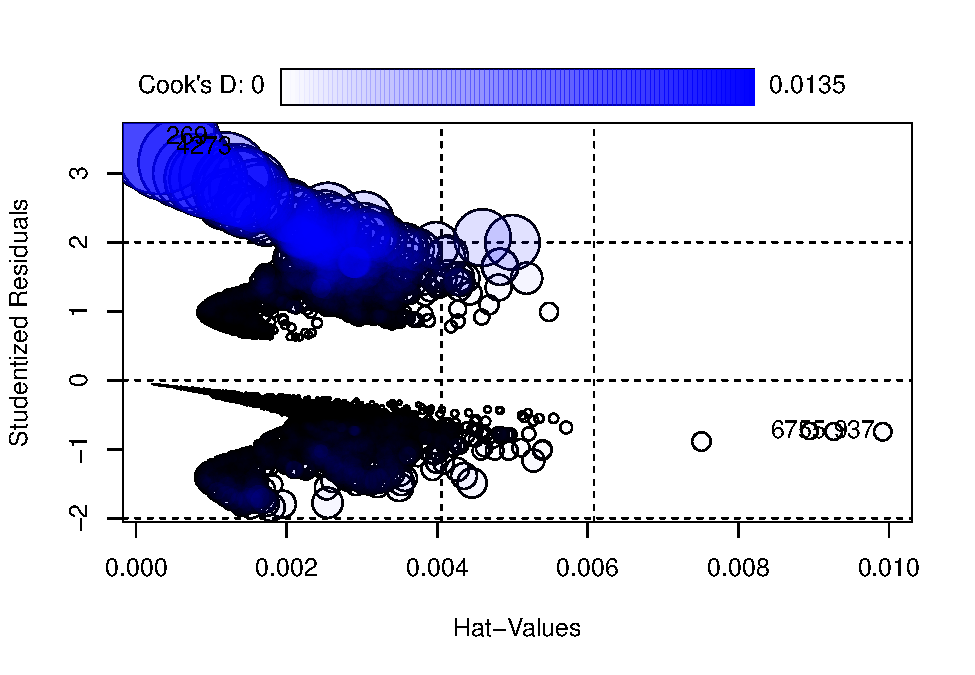
\includegraphics{AdriàCasanova-VíctorGarcia-ZhengyongJi_files/figure-latex/Final Influential data analysis-1.pdf}

\begin{Shaded}
\begin{Highlighting}[]
\NormalTok{influent}
\end{Highlighting}
\end{Shaded}

\begin{verbatim}
##             CookD
## 269  0.0134537052
## 937  0.0003234289
## 4273 0.0119056685
## 6755 0.0002981121
\end{verbatim}

\begin{Shaded}
\begin{Highlighting}[]
\CommentTok{\# Calculate D\textquotesingle{}s threshold}
\NormalTok{D\_thresh }\OtherTok{\textless{}{-}} \DecValTok{2}\SpecialCharTok{/}\FunctionTok{sqrt}\NormalTok{(}\FunctionTok{dim}\NormalTok{(train)[}\DecValTok{1}\NormalTok{])}
\NormalTok{D\_thresh}
\end{Highlighting}
\end{Shaded}

\begin{verbatim}
## [1] 0.02848436
\end{verbatim}

\begin{Shaded}
\begin{Highlighting}[]
\CommentTok{\# The most influential observations are the 269 and 4273,}
\CommentTok{\# which are the ones with the biggest Cook\textquotesingle{}s distance.}
\CommentTok{\# Nonetheless, any of them is a multivariate outlier.}
\FunctionTok{sum}\NormalTok{(outliers }\SpecialCharTok{==} \DecValTok{269}\NormalTok{)}
\end{Highlighting}
\end{Shaded}

\begin{verbatim}
## [1] 0
\end{verbatim}

\begin{Shaded}
\begin{Highlighting}[]
\FunctionTok{sum}\NormalTok{(outliers }\SpecialCharTok{==} \DecValTok{4273}\NormalTok{)}
\end{Highlighting}
\end{Shaded}

\begin{verbatim}
## [1] 0
\end{verbatim}

\begin{Shaded}
\begin{Highlighting}[]
\NormalTok{df}\SpecialCharTok{$}\NormalTok{Churn[}\DecValTok{269}\NormalTok{]}
\end{Highlighting}
\end{Shaded}

\begin{verbatim}
## [1] Yes
## Levels: No Yes
\end{verbatim}

\begin{Shaded}
\begin{Highlighting}[]
\NormalTok{df}\SpecialCharTok{$}\NormalTok{Churn[}\DecValTok{4273}\NormalTok{]}
\end{Highlighting}
\end{Shaded}

\begin{verbatim}
## [1] Yes
## Levels: No Yes
\end{verbatim}

\begin{Shaded}
\begin{Highlighting}[]
\CommentTok{\# Neither is a univariate outlier in tenure and}
\CommentTok{\# TotalCharges when analyzed inside their target\textquotesingle{}s}
\CommentTok{\# category.}
\FunctionTok{sum}\NormalTok{(}\FunctionTok{Boxplot}\NormalTok{(df}\SpecialCharTok{$}\NormalTok{tenure[df}\SpecialCharTok{$}\NormalTok{Churn }\SpecialCharTok{==} \StringTok{"Yes"}\NormalTok{]) }\SpecialCharTok{==} \DecValTok{269}\NormalTok{)}
\end{Highlighting}
\end{Shaded}

\begin{verbatim}
## [1] 0
\end{verbatim}

\begin{Shaded}
\begin{Highlighting}[]
\FunctionTok{sum}\NormalTok{(}\FunctionTok{Boxplot}\NormalTok{(df}\SpecialCharTok{$}\NormalTok{tenure[df}\SpecialCharTok{$}\NormalTok{Churn }\SpecialCharTok{==} \StringTok{"Yes"}\NormalTok{]) }\SpecialCharTok{==} \DecValTok{4273}\NormalTok{)}
\end{Highlighting}
\end{Shaded}

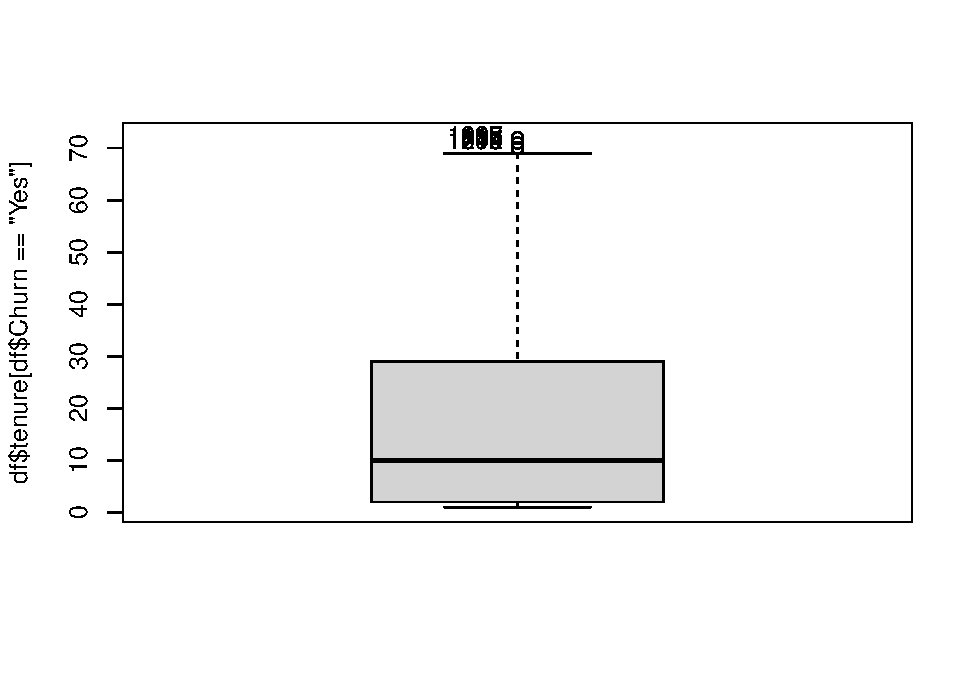
\includegraphics{AdriàCasanova-VíctorGarcia-ZhengyongJi_files/figure-latex/Final Influential data analysis-2.pdf}

\begin{verbatim}
## [1] 0
\end{verbatim}

\begin{Shaded}
\begin{Highlighting}[]
\FunctionTok{sum}\NormalTok{(}\FunctionTok{Boxplot}\NormalTok{(df}\SpecialCharTok{$}\NormalTok{MonthlyCharges[df}\SpecialCharTok{$}\NormalTok{Churn }\SpecialCharTok{==} \StringTok{"Yes"}\NormalTok{]) }\SpecialCharTok{==} \DecValTok{269}\NormalTok{)}
\end{Highlighting}
\end{Shaded}

\begin{verbatim}
## [1] 0
\end{verbatim}

\begin{Shaded}
\begin{Highlighting}[]
\FunctionTok{sum}\NormalTok{(}\FunctionTok{Boxplot}\NormalTok{(df}\SpecialCharTok{$}\NormalTok{MonthlyCharges[df}\SpecialCharTok{$}\NormalTok{Churn }\SpecialCharTok{==} \StringTok{"Yes"}\NormalTok{]) }\SpecialCharTok{==} \DecValTok{4273}\NormalTok{)}
\end{Highlighting}
\end{Shaded}

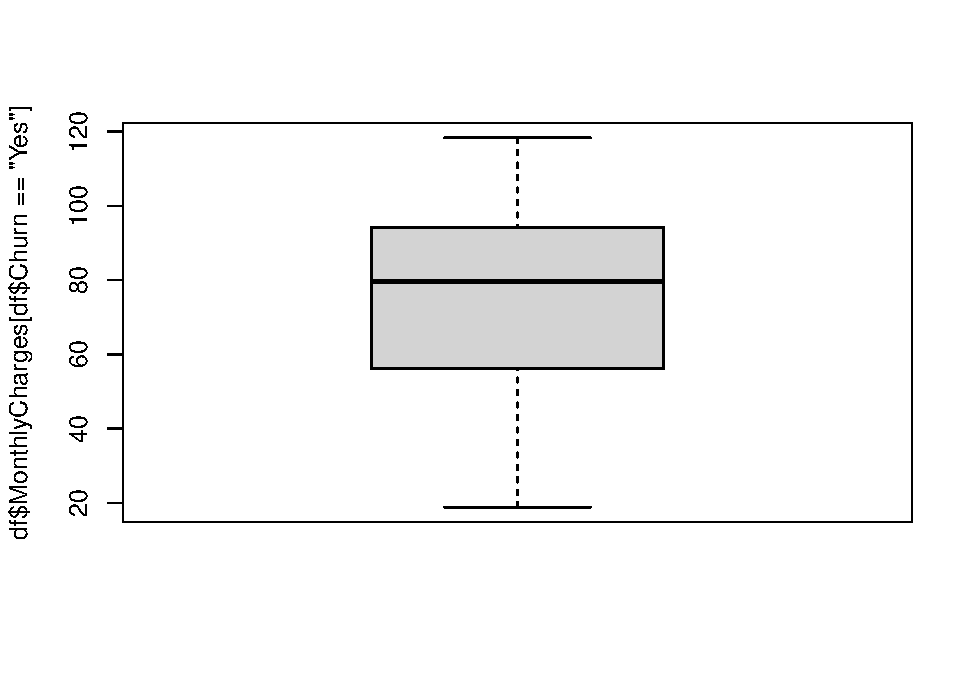
\includegraphics{AdriàCasanova-VíctorGarcia-ZhengyongJi_files/figure-latex/Final Influential data analysis-3.pdf}

\begin{verbatim}
## [1] 0
\end{verbatim}

\begin{Shaded}
\begin{Highlighting}[]
\FunctionTok{sum}\NormalTok{(}\FunctionTok{Boxplot}\NormalTok{(df}\SpecialCharTok{$}\NormalTok{TotalCharges[df}\SpecialCharTok{$}\NormalTok{Churn }\SpecialCharTok{==} \StringTok{"Yes"}\NormalTok{]) }\SpecialCharTok{==} \DecValTok{269}\NormalTok{)}
\end{Highlighting}
\end{Shaded}

\begin{verbatim}
## [1] 0
\end{verbatim}

\begin{Shaded}
\begin{Highlighting}[]
\FunctionTok{sum}\NormalTok{(}\FunctionTok{Boxplot}\NormalTok{(df}\SpecialCharTok{$}\NormalTok{TotalCharges[df}\SpecialCharTok{$}\NormalTok{Churn }\SpecialCharTok{==} \StringTok{"Yes"}\NormalTok{]) }\SpecialCharTok{==} \DecValTok{4273}\NormalTok{)}
\end{Highlighting}
\end{Shaded}

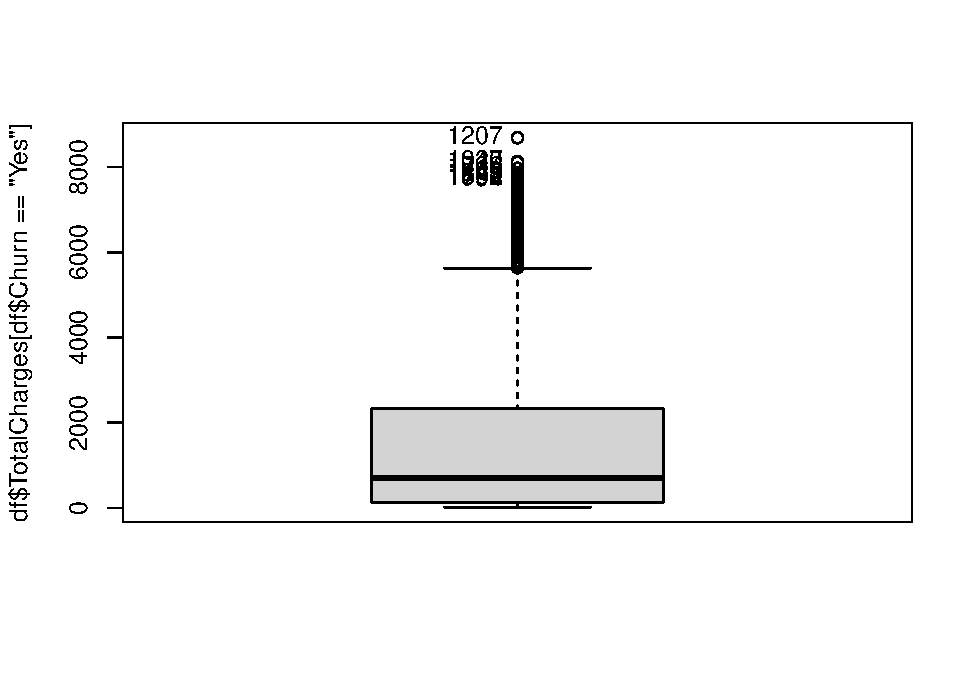
\includegraphics{AdriàCasanova-VíctorGarcia-ZhengyongJi_files/figure-latex/Final Influential data analysis-4.pdf}

\begin{verbatim}
## [1] 0
\end{verbatim}

Observations 269 and 4273 may be influential points, but both of them
are smaller than the threshold. Any of these are multivariate outliers
or severe outliers of a numerical variable when looked in their category
of Churn. They are not neither globally, since we saw in the
preprocessing that there were no severe outliers. Hence, we won't remove
any of them.

\hypertarget{goodness-of-fit}{%
\section{6. Goodness of fit}\label{goodness-of-fit}}

\begin{Shaded}
\begin{Highlighting}[]
\FunctionTok{PseudoR2}\NormalTok{(m5, }\AttributeTok{which =} \StringTok{"McFadden"}\NormalTok{)}
\end{Highlighting}
\end{Shaded}

\begin{verbatim}
##  McFadden 
## 0.2830884
\end{verbatim}

The R2 of McFadden is not excellent, but at least it is acceptable. Let
us check the residual plots.

\begin{Shaded}
\begin{Highlighting}[]
\FunctionTok{residualPlots}\NormalTok{(m5)}
\end{Highlighting}
\end{Shaded}

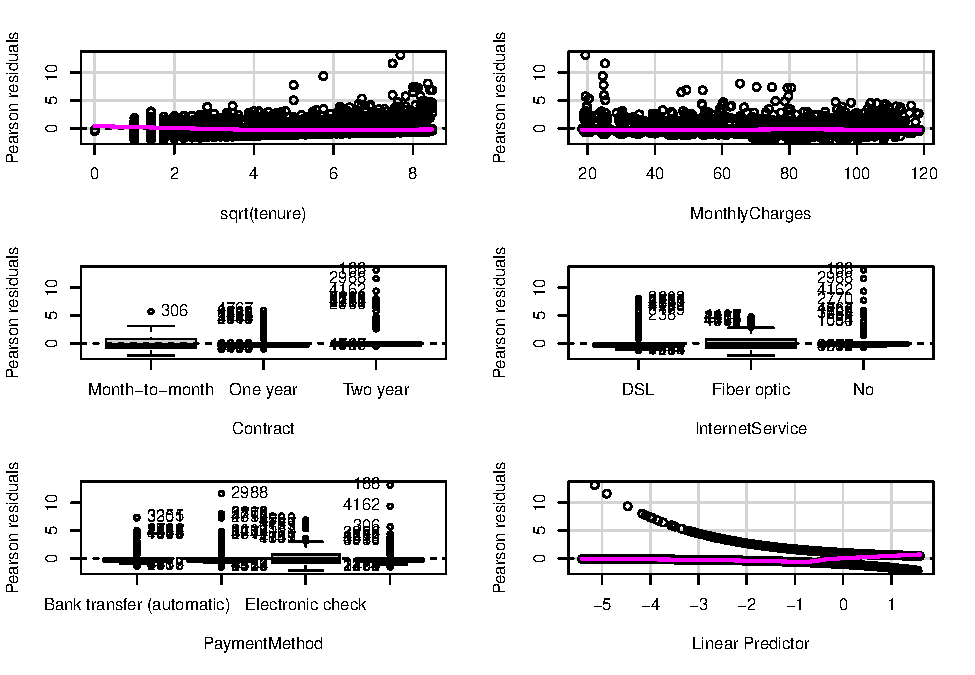
\includegraphics{AdriàCasanova-VíctorGarcia-ZhengyongJi_files/figure-latex/Residual plots-1.pdf}

\begin{verbatim}
##                 Test stat Pr(>|Test stat|)    
## sqrt(tenure)       21.586        3.384e-06 ***
## MonthlyCharges     21.877        2.907e-06 ***
## Contract                                      
## InternetService                               
## PaymentMethod                                 
## ---
## Signif. codes:  0 '***' 0.001 '**' 0.01 '*' 0.05 '.' 0.1 ' ' 1
\end{verbatim}

\begin{Shaded}
\begin{Highlighting}[]
\CommentTok{\# Outliers in the residual plots might be caused, in part,}
\CommentTok{\# by unbalanced data}
\FunctionTok{prop.table}\NormalTok{(}\FunctionTok{table}\NormalTok{(df}\SpecialCharTok{$}\NormalTok{Contract))}
\end{Highlighting}
\end{Shaded}

\begin{verbatim}
## 
## Month-to-month       One year       Two year 
##      0.5501917      0.2091438      0.2406645
\end{verbatim}

\begin{Shaded}
\begin{Highlighting}[]
\FunctionTok{prop.table}\NormalTok{(}\FunctionTok{table}\NormalTok{(df}\SpecialCharTok{$}\NormalTok{InternetService))}
\end{Highlighting}
\end{Shaded}

\begin{verbatim}
## 
##         DSL Fiber optic          No 
##   0.3437456   0.4395854   0.2166690
\end{verbatim}

\begin{Shaded}
\begin{Highlighting}[]
\FunctionTok{prop.table}\NormalTok{(}\FunctionTok{table}\NormalTok{(df}\SpecialCharTok{$}\NormalTok{PaymentMethod))}
\end{Highlighting}
\end{Shaded}

\begin{verbatim}
## 
## Bank transfer (automatic)   Credit card (automatic)          Electronic check 
##                 0.2192248                 0.2161011                 0.3357944 
##              Mailed check 
##                 0.2288797
\end{verbatim}

In the residual plots we see that all levels in the model contain severe
outliers, except for ``Month-to-month'' (there is only 1 outlier).
However, those points do not seem to affect the Pearson residuals
distributions, which are all close to zero as expected. Moreover, they
might be caused by unbalanced data.

\begin{Shaded}
\begin{Highlighting}[]
\NormalTok{m5.mout }\OtherTok{=} \FunctionTok{glm}\NormalTok{(Churn }\SpecialCharTok{\textasciitilde{}} \FunctionTok{sqrt}\NormalTok{(tenure) }\SpecialCharTok{+}\NormalTok{ MonthlyCharges }\SpecialCharTok{+}\NormalTok{ Contract }\SpecialCharTok{+}
\NormalTok{    InternetService }\SpecialCharTok{+}\NormalTok{ PaymentMethod, }\AttributeTok{data =}\NormalTok{ train[}\SpecialCharTok{{-}}\NormalTok{outliers,}
\NormalTok{    ], }\AttributeTok{family =}\NormalTok{ binomial)}
\FunctionTok{residualPlots}\NormalTok{(m5.mout)}
\end{Highlighting}
\end{Shaded}

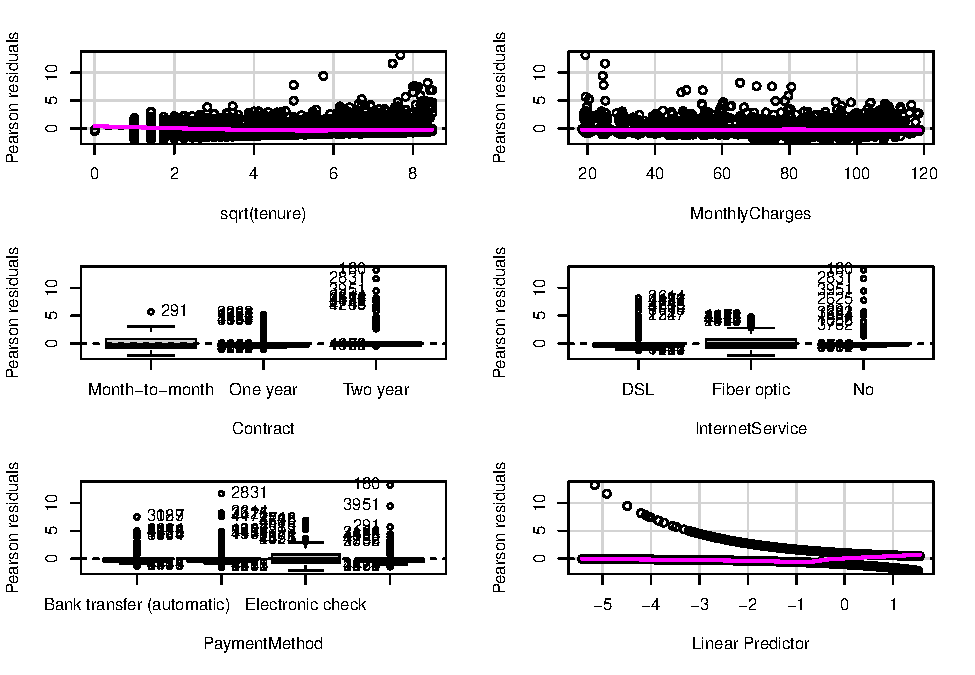
\includegraphics{AdriàCasanova-VíctorGarcia-ZhengyongJi_files/figure-latex/m5.out-1.pdf}

\begin{verbatim}
##                 Test stat Pr(>|Test stat|)    
## sqrt(tenure)       20.256        6.775e-06 ***
## MonthlyCharges     19.519        9.959e-06 ***
## Contract                                      
## InternetService                               
## PaymentMethod                                 
## ---
## Signif. codes:  0 '***' 0.001 '**' 0.01 '*' 0.05 '.' 0.1 ' ' 1
\end{verbatim}

To try to remove those outliers from the categorical variables we remove
all multivariate outliers. This gives us an alternative model (m5.mout)
that we cannot compare using BIC or other measure of fitness as the
models do not have the same cardinality. However, the new model still
contains outliers in the residual plot, so we consider that it is better
not to remove the multivariate outliers. This backs up the hypothesis of
unbalanced data causing outliers in the Pearson residuals.

\hypertarget{model-prediction}{%
\subsection{Model prediction}\label{model-prediction}}

Once we have our final model m5 we can predict the values of Churn on
the test dataset.

\begin{Shaded}
\begin{Highlighting}[]
\CommentTok{\# First, we compute the probability of Churn for each}
\CommentTok{\# observation (from test) with predict function.}
\NormalTok{predictions }\OtherTok{=} \FunctionTok{predict}\NormalTok{(m5, test[}\SpecialCharTok{{-}}\DecValTok{20}\NormalTok{], }\AttributeTok{type =} \StringTok{"response"}\NormalTok{)}

\CommentTok{\# Then, for those that have a probability higher than 0.5,}
\CommentTok{\# we can consider Churn == \textquotesingle{}Yes\textquotesingle{}}
\NormalTok{probability }\OtherTok{=} \FunctionTok{factor}\NormalTok{(}\FunctionTok{as.character}\NormalTok{(}\FunctionTok{ifelse}\NormalTok{(predictions }\SpecialCharTok{\textgreater{}=} \FloatTok{0.5}\NormalTok{,}
    \StringTok{"Yes"}\NormalTok{, }\StringTok{"No"}\NormalTok{)))}

\CommentTok{\# Finally, compute the Confusion Matrix of predicted result}
\NormalTok{confusion.mat }\OtherTok{\textless{}{-}} \FunctionTok{confusionMatrix}\NormalTok{(probability, test}\SpecialCharTok{$}\NormalTok{Churn, }\AttributeTok{mode =} \StringTok{"everything"}\NormalTok{,}
    \AttributeTok{positive =} \StringTok{"Yes"}\NormalTok{)}
\NormalTok{confusion.mat}
\end{Highlighting}
\end{Shaded}

\begin{verbatim}
## Confusion Matrix and Statistics
## 
##           Reference
## Prediction   No  Yes
##        No  1395  279
##        Yes  157  282
##                                           
##                Accuracy : 0.7937          
##                  95% CI : (0.7758, 0.8107)
##     No Information Rate : 0.7345          
##     P-Value [Acc > NIR] : 1.548e-10       
##                                           
##                   Kappa : 0.4315          
##                                           
##  Mcnemar's Test P-Value : 6.838e-09       
##                                           
##             Sensitivity : 0.5027          
##             Specificity : 0.8988          
##          Pos Pred Value : 0.6424          
##          Neg Pred Value : 0.8333          
##               Precision : 0.6424          
##                  Recall : 0.5027          
##                      F1 : 0.5640          
##              Prevalence : 0.2655          
##          Detection Rate : 0.1335          
##    Detection Prevalence : 0.2078          
##       Balanced Accuracy : 0.7008          
##                                           
##        'Positive' Class : Yes             
## 
\end{verbatim}

\begin{Shaded}
\begin{Highlighting}[]
\FunctionTok{roc.curve}\NormalTok{(test}\SpecialCharTok{$}\NormalTok{Churn, probability)}
\end{Highlighting}
\end{Shaded}

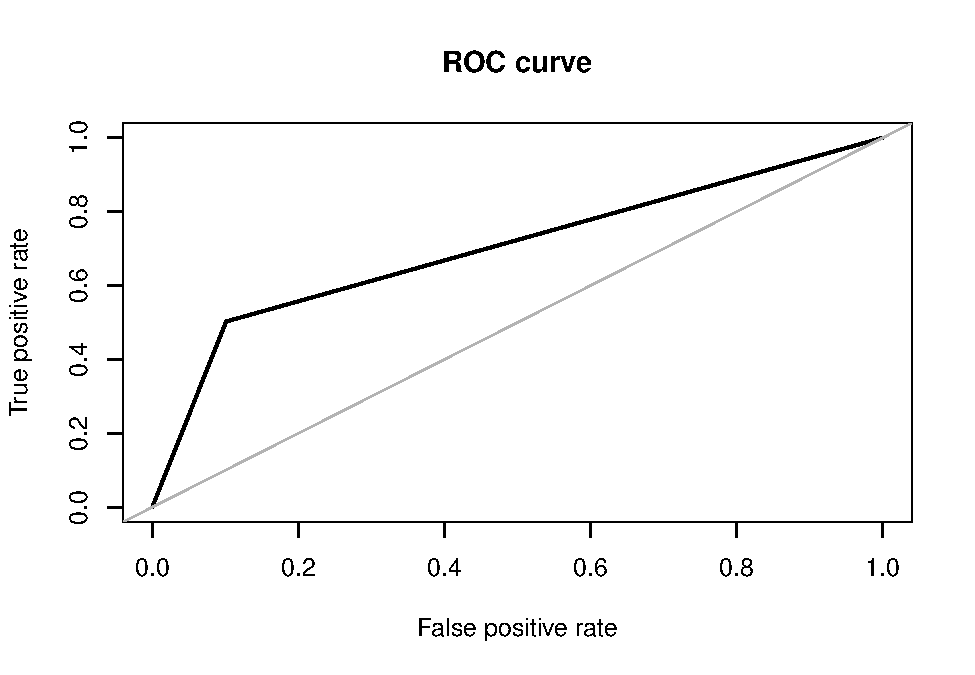
\includegraphics{AdriàCasanova-VíctorGarcia-ZhengyongJi_files/figure-latex/predict()-1.pdf}

\begin{verbatim}
## Area under the curve (AUC): 0.701
\end{verbatim}

With the predicted values of the target, we can also study the goodness
of fit of the model m5 through the confusion matrix. The most typical
measure obtained from this matrix is the accuracy, but in our case it is
not reliable because we have unbalanced data. Hence, we resort to the
F1-score, a harmonic mean that is less influenced by unbalanced data. We
got a value of 56\%, which is not great, but it is not a worthless
model. This is confirmed by the ROC curve plotted above, with AUC =
0.70.

Finally, we compare m5 with the null model to see the improvement we
have obtained.

\begin{Shaded}
\begin{Highlighting}[]
\NormalTok{m.null }\OtherTok{=} \FunctionTok{glm}\NormalTok{(Churn }\SpecialCharTok{\textasciitilde{}} \DecValTok{1}\NormalTok{, }\AttributeTok{data =}\NormalTok{ train, }\AttributeTok{family =}\NormalTok{ binomial)}

\FunctionTok{BIC}\NormalTok{(m5, m.null)}
\end{Highlighting}
\end{Shaded}

\begin{verbatim}
##        df      BIC
## m5     10 4174.603
## m.null  1 5712.933
\end{verbatim}

BIC coefficient decreased from 5712 to 4174. So we improve the
predictive capability.

\hypertarget{model-interpretation}{%
\section{7. Model interpretation}\label{model-interpretation}}

Finally, let's summarize and interpret our final model.

\begin{Shaded}
\begin{Highlighting}[]
\NormalTok{m5 }\OtherTok{=} \FunctionTok{glm}\NormalTok{(Churn }\SpecialCharTok{\textasciitilde{}} \FunctionTok{sqrt}\NormalTok{(tenure) }\SpecialCharTok{+}\NormalTok{ MonthlyCharges }\SpecialCharTok{+}\NormalTok{ Contract }\SpecialCharTok{+}\NormalTok{ InternetService }\SpecialCharTok{+}
\NormalTok{    PaymentMethod, }\AttributeTok{data =}\NormalTok{ train, }\AttributeTok{family =}\NormalTok{ binomial)}

\FunctionTok{summary}\NormalTok{(m5)}
\end{Highlighting}
\end{Shaded}

\begin{verbatim}
## 
## Call:
## glm(formula = Churn ~ sqrt(tenure) + MonthlyCharges + Contract + 
##     InternetService + PaymentMethod, family = binomial, data = train)
## 
## Coefficients:
##                                       Estimate Std. Error z value Pr(>|z|)    
## (Intercept)                          -0.302267   0.213978  -1.413 0.157771    
## sqrt(tenure)                         -0.328520   0.022733 -14.451  < 2e-16 ***
## MonthlyCharges                        0.008831   0.003666   2.409 0.015984 *  
## ContractOne year                     -0.831241   0.127318  -6.529 6.63e-11 ***
## ContractTwo year                     -1.707955   0.201971  -8.456  < 2e-16 ***
## InternetServiceFiber optic            0.843216   0.155490   5.423 5.86e-08 ***
## InternetServiceNo                    -0.674397   0.185458  -3.636 0.000276 ***
## PaymentMethodCredit card (automatic)  0.016257   0.135680   0.120 0.904625    
## PaymentMethodElectronic check         0.482651   0.112957   4.273 1.93e-05 ***
## PaymentMethodMailed check            -0.116088   0.137387  -0.845 0.398128    
## ---
## Signif. codes:  0 '***' 0.001 '**' 0.01 '*' 0.05 '.' 0.1 ' ' 1
## 
## (Dispersion parameter for binomial family taken to be 1)
## 
##     Null deviance: 5704.4  on 4929  degrees of freedom
## Residual deviance: 4089.6  on 4920  degrees of freedom
## AIC: 4109.6
## 
## Number of Fisher Scoring iterations: 6
\end{verbatim}

\begin{Shaded}
\begin{Highlighting}[]
\FunctionTok{sort}\NormalTok{(}\FunctionTok{exp}\NormalTok{(m5}\SpecialCharTok{$}\NormalTok{coefficients), }\AttributeTok{decreasing =} \ConstantTok{TRUE}\NormalTok{)}
\end{Highlighting}
\end{Shaded}

\begin{verbatim}
##           InternetServiceFiber optic        PaymentMethodElectronic check 
##                            2.3238275                            1.6203637 
## PaymentMethodCredit card (automatic)                       MonthlyCharges 
##                            1.0163902                            1.0088706 
##            PaymentMethodMailed check                          (Intercept) 
##                            0.8903972                            0.7391410 
##                         sqrt(tenure)                    InternetServiceNo 
##                            0.7199885                            0.5094636 
##                     ContractOne year                     ContractTwo year 
##                            0.4355085                            0.1812361
\end{verbatim}

The model is composed by the tenure of the customer, the bill they pay
monthly, the contract period that they have with the company, the
internet service they own and the payment method.

Bear in mind that 1 denotes ``client churned'' and 0 denotes ``client
did not churn'', where clients with a lower linear predictor are less
likely to leave the company.

As a consequence, loyalty (more tenure), reduces the odds to churn while
MonthlyCharges increases it. Also, with categorical variables we see
that costumers with a Fiber optic double the odds to churn with respect
to costumers with a DSL service (reference category for
``InternetService'') all else being equal.

Additionally, paying with Electronic check, instead of a ``bank
transfer'' increases by 62\% the odds to churn, all else being equal.
Other payment methods do not have a big impact on the Churn.

More importantly, it seems that having long contract periods is very
important to reduce the odds to churn, as clients that have a biannual
contract have approximately 99\% less odds of not to churn compared to
the ones that have a monthly contract, all else being equal.

Additionally, not having internet is also important, as those clients
have 50\% less odds to churn with respect to the ones that have a DSL
service all else being equal. This may indicate that this group of
individuals prefer a more basic service but are more stable.

\hypertarget{conclusions}{%
\section{8. Conclusions}\label{conclusions}}

In this project we have created a generalized linear model that predicts
the probability to churn using \{tenure, MonthlyCharges, Contract,
InternetService, PaymentMethod\}, all these predictors are explained
with detail in the previous chapter. In total, our model predictors are
composed of 2 numerical features and 3 categorical variables, with
tenure transformed and no interactions.

The indicator of performance of this model shows a F1 score of 0.5640,
and Area under the Curve (AUC) of 0.701. Accuracy is not considered
because of the dataset's imbalance, indeed many people churned. As a
consequence our confusion matrix, found below, contain more errors than
True Positives.

\begin{verbatim}
##           Reference
## Prediction   No  Yes
##        No  1395  279
##        Yes  157  282
\end{verbatim}

Although our model is not perfect, we are searching a balance between
simplicity and accuracy, considering the trade-off associated with
adding more variables and interactions. Indeed that would improve the
fitness, but with the cost of increasing the parameters and complexity
of the model, which lately make it harder to be interpreted.

As future work, we can try to study different methods to balance the
data set, either undersampling the category of people who did not churn
or uppersampling the complementary category.

\newpage

\hypertarget{annex}{%
\section{Annex}\label{annex}}

\hypertarget{expanded-profiling-of-the-target-with-the-profiling-method}{%
\subsection{Expanded profiling of the target with the ``profiling()''
method}\label{expanded-profiling-of-the-target-with-the-profiling-method}}

\begin{Shaded}
\begin{Highlighting}[]
\CommentTok{\# Analysis of all variables except the ID}
\FunctionTok{profiling}\NormalTok{(df[}\SpecialCharTok{{-}}\FunctionTok{c}\NormalTok{(}\FunctionTok{grep}\NormalTok{(}\StringTok{"customerID"}\NormalTok{, }\FunctionTok{names}\NormalTok{(df)), }\FunctionTok{grep}\NormalTok{(}\StringTok{"Churn"}\NormalTok{,}
    \FunctionTok{names}\NormalTok{(df)))], df}\SpecialCharTok{$}\NormalTok{Churn, }\StringTok{"Churn"}\NormalTok{)}
\end{Highlighting}
\end{Shaded}

\begin{verbatim}
## [1] "Variable gender"
## [1] "Categories=" "Female"      "Male"
\end{verbatim}

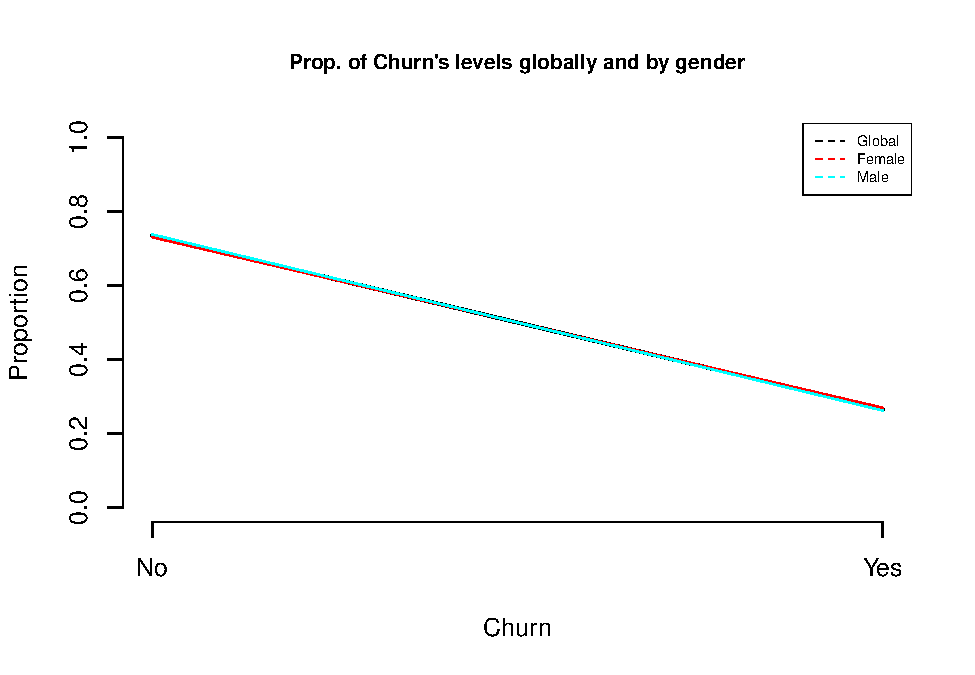
\includegraphics{AdriàCasanova-VíctorGarcia-ZhengyongJi_files/figure-latex/Karinas profiling method not hidden-1.pdf}
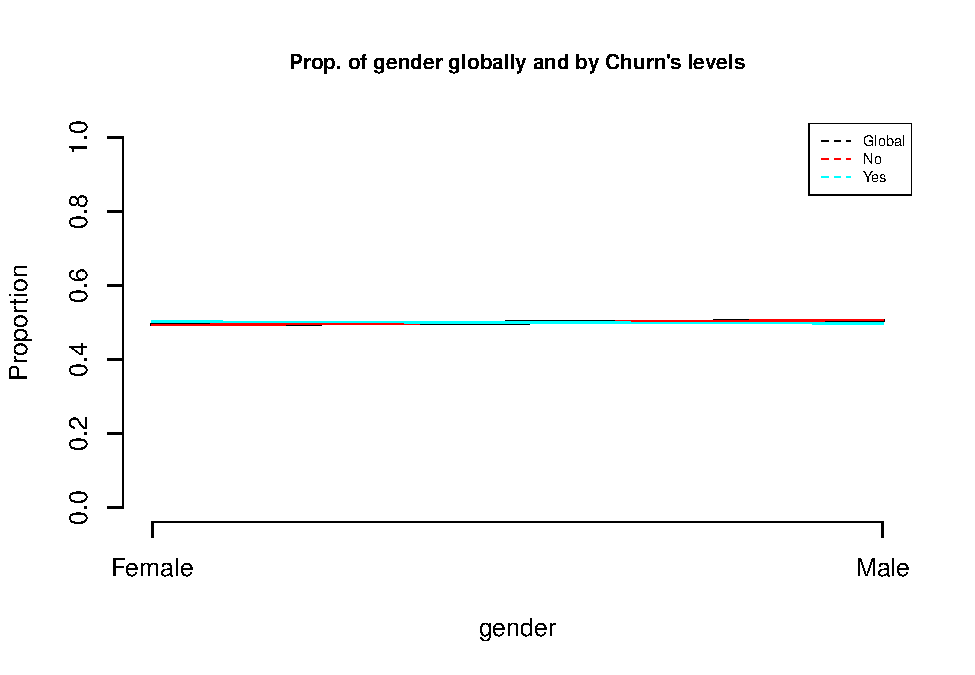
\includegraphics{AdriàCasanova-VíctorGarcia-ZhengyongJi_files/figure-latex/Karinas profiling method not hidden-2.pdf}

\begin{verbatim}
## [1] "Cross Table:"
##         P
##            No  Yes
##   Female 2549  939
##   Male   2625  930
## [1] "Distributions by columns:"
##      
## P        Female      Male
##   No  0.7307913 0.7383966
##   Yes 0.2692087 0.2616034
## [1] "Chi^2 test: "
## 
##  Pearson's Chi-squared test with Yates' continuity correction
## 
## data:  dades[, k] and as.factor(P)
## X-squared = 0.48408, df = 1, p-value = 0.4866
## 
## [1] "ValorTestXquali:"
## $rowpf
##      Xquali
## P        Female      Male
##   No  0.4926556 0.5073444
##   Yes 0.5024077 0.4975923
## 
## $vtest
##      Xquali
## P         Female       Male
##   No  -0.7227493  0.7227493
##   Yes  0.7227493 -0.7227493
## 
## $pval
##      Xquali
## P       Female     Male
##   No  0.234917 0.234917
##   Yes 0.234917 0.234917
## 
## [1] "Variable SeniorCitizen"
## [1] "Categories=" "Yes"         "No"
\end{verbatim}

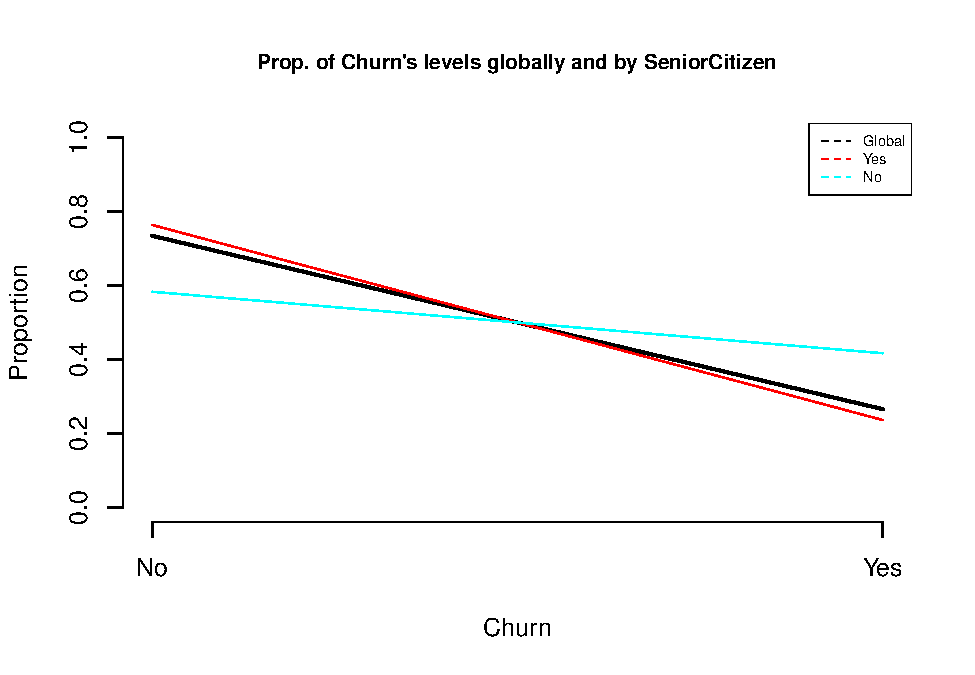
\includegraphics{AdriàCasanova-VíctorGarcia-ZhengyongJi_files/figure-latex/Karinas profiling method not hidden-3.pdf}
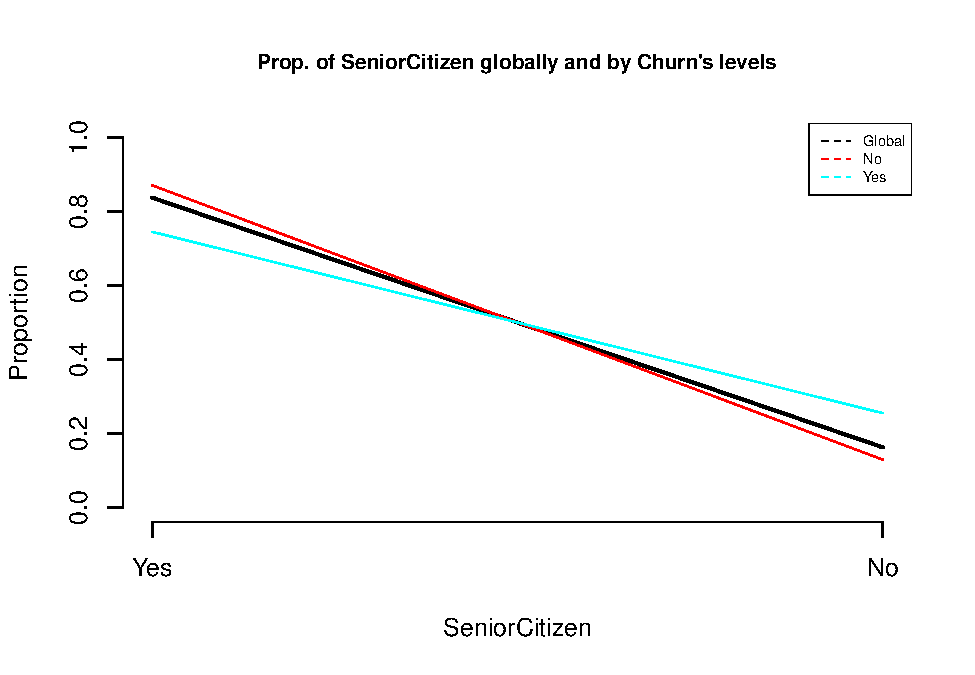
\includegraphics{AdriàCasanova-VíctorGarcia-ZhengyongJi_files/figure-latex/Karinas profiling method not hidden-4.pdf}

\begin{verbatim}
## [1] "Cross Table:"
##      P
##         No  Yes
##   Yes 4508 1393
##   No   666  476
## [1] "Distributions by columns:"
##      
## P           Yes        No
##   No  0.7639383 0.5831874
##   Yes 0.2360617 0.4168126
## [1] "Chi^2 test: "
## 
##  Pearson's Chi-squared test with Yates' continuity correction
## 
## data:  dades[, k] and as.factor(P)
## X-squared = 159.43, df = 1, p-value < 2.2e-16
## 
## [1] "ValorTestXquali:"
## $rowpf
##      Xquali
## P           Yes        No
##   No  0.8712795 0.1287205
##   Yes 0.7453184 0.2546816
## 
## $vtest
##      Xquali
## P           Yes        No
##   No   12.66302 -12.66302
##   Yes -12.66302  12.66302
## 
## $pval
##      Xquali
## P              Yes           No
##   No  4.738952e-37 0.000000e+00
##   Yes 0.000000e+00 4.738952e-37
## 
## [1] "Variable Partner"
## [1] "Categories=" "No"          "Yes"
\end{verbatim}

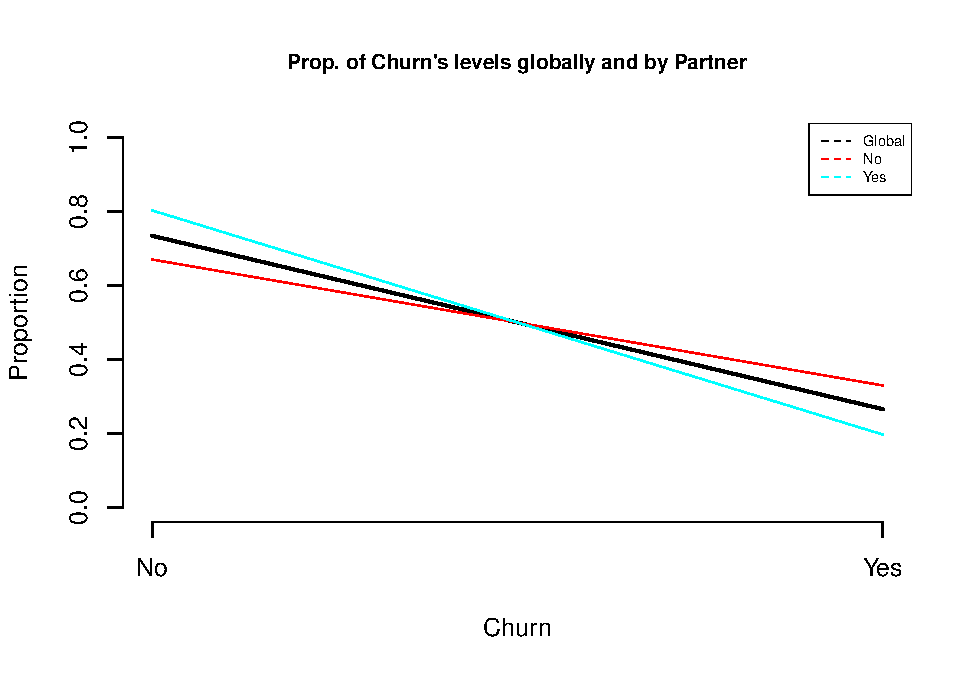
\includegraphics{AdriàCasanova-VíctorGarcia-ZhengyongJi_files/figure-latex/Karinas profiling method not hidden-5.pdf}
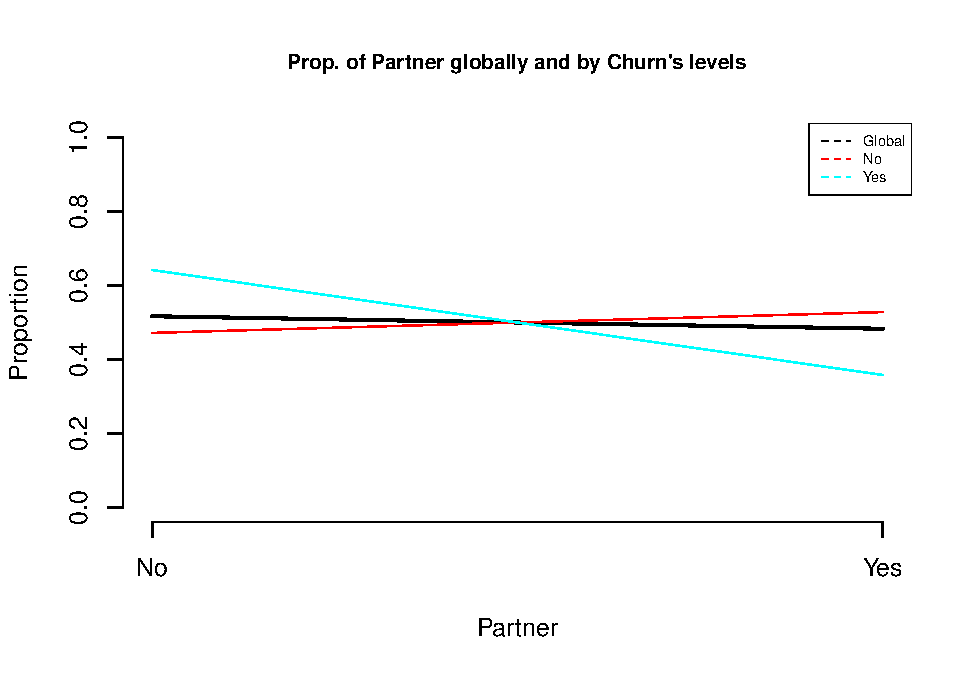
\includegraphics{AdriàCasanova-VíctorGarcia-ZhengyongJi_files/figure-latex/Karinas profiling method not hidden-6.pdf}

\begin{verbatim}
## [1] "Cross Table:"
##      P
##         No  Yes
##   No  2441 1200
##   Yes 2733  669
## [1] "Distributions by columns:"
##      
## P            No       Yes
##   No  0.6704202 0.8033510
##   Yes 0.3295798 0.1966490
## [1] "Chi^2 test: "
## 
##  Pearson's Chi-squared test with Yates' continuity correction
## 
## data:  dades[, k] and as.factor(P)
## X-squared = 158.73, df = 1, p-value < 2.2e-16
## 
## [1] "ValorTestXquali:"
## $rowpf
##      Xquali
## P            No       Yes
##   No  0.4717820 0.5282180
##   Yes 0.6420546 0.3579454
## 
## $vtest
##      Xquali
## P            No       Yes
##   No  -12.62595  12.62595
##   Yes  12.62595 -12.62595
## 
## $pval
##      Xquali
## P               No          Yes
##   No  0.000000e+00 7.595183e-37
##   Yes 7.595183e-37 0.000000e+00
## 
## [1] "Variable Dependents"
## [1] "Categories=" "No"          "Yes"
\end{verbatim}

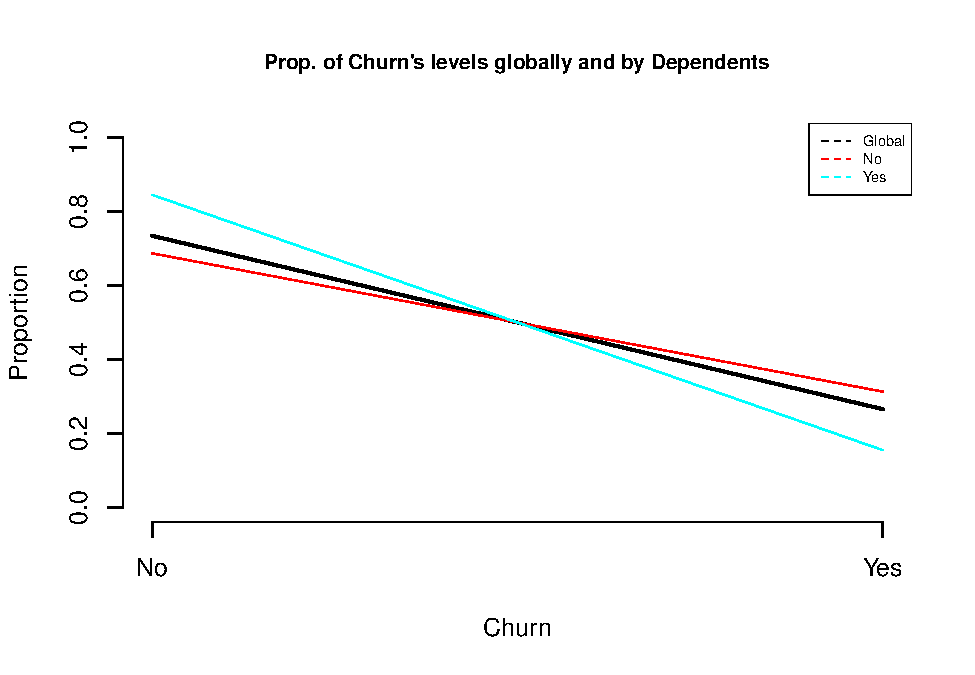
\includegraphics{AdriàCasanova-VíctorGarcia-ZhengyongJi_files/figure-latex/Karinas profiling method not hidden-7.pdf}
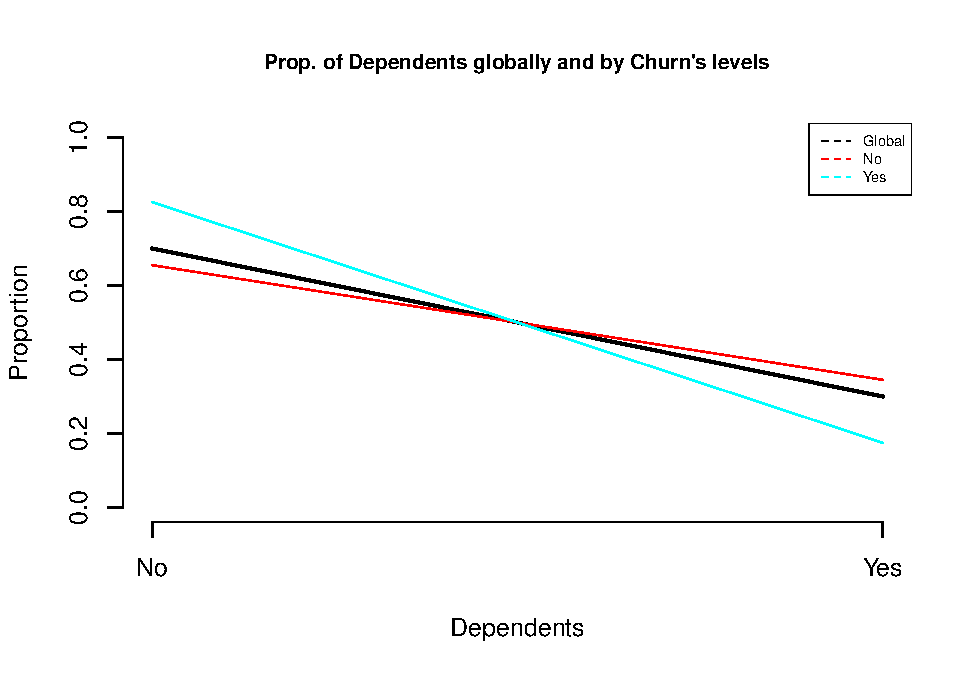
\includegraphics{AdriàCasanova-VíctorGarcia-ZhengyongJi_files/figure-latex/Karinas profiling method not hidden-8.pdf}

\begin{verbatim}
## [1] "Cross Table:"
##      P
##         No  Yes
##   No  3390 1543
##   Yes 1784  326
## [1] "Distributions by columns:"
##      
## P            No       Yes
##   No  0.6872086 0.8454976
##   Yes 0.3127914 0.1545024
## [1] "Chi^2 test: "
## 
##  Pearson's Chi-squared test with Yates' continuity correction
## 
## data:  dades[, k] and as.factor(P)
## X-squared = 189.13, df = 1, p-value < 2.2e-16
## 
## [1] "ValorTestXquali:"
## $rowpf
##      Xquali
## P            No       Yes
##   No  0.6551991 0.3448009
##   Yes 0.8255752 0.1744248
## 
## $vtest
##      Xquali
## P            No       Yes
##   No  -13.78188  13.78188
##   Yes  13.78188 -13.78188
## 
## $pval
##      Xquali
## P               No          Yes
##   No  0.000000e+00 1.638041e-43
##   Yes 1.638041e-43 0.000000e+00
## 
## [1] "Analysis by level of : tenure"
\end{verbatim}

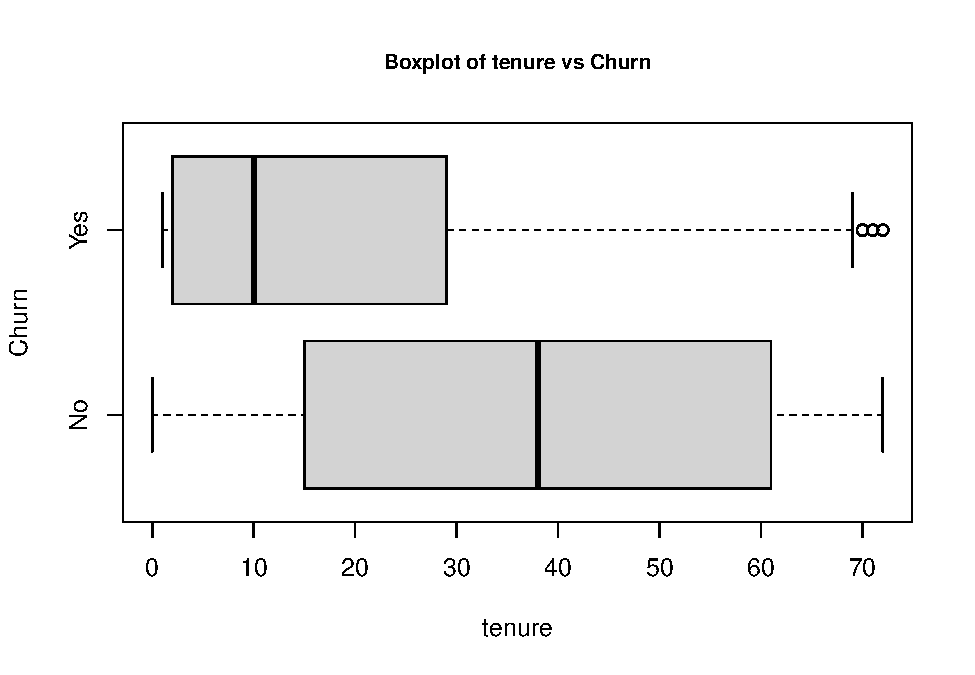
\includegraphics{AdriàCasanova-VíctorGarcia-ZhengyongJi_files/figure-latex/Karinas profiling method not hidden-9.pdf}
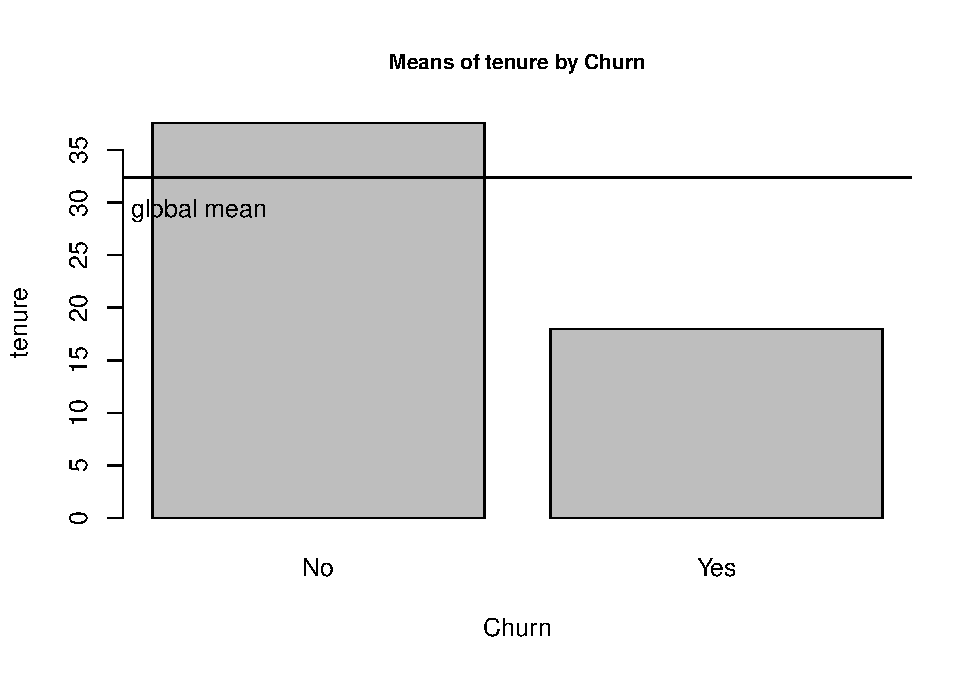
\includegraphics{AdriàCasanova-VíctorGarcia-ZhengyongJi_files/figure-latex/Karinas profiling method not hidden-10.pdf}

\begin{verbatim}
## [1] "Statistics by group:"
##    Min. 1st Qu.  Median    Mean 3rd Qu.    Max. 
##    0.00   15.00   38.00   37.57   61.00   72.00 
##    Min. 1st Qu.  Median    Mean 3rd Qu.    Max. 
##    1.00    2.00   10.00   17.98   29.00   72.00 
## [1] "p-valueANOVA: 1.19549454726051e-232"
## [1] "p-value Kruskal-Wallis: 2.41914018186156e-208"
## [1] "p-values ValorsTest: "
##            No           Yes 
## 2.081921e-181  0.000000e+00 
## [1] "Variable PhoneService"
## [1] "Categories=" "No"          "Yes"
\end{verbatim}

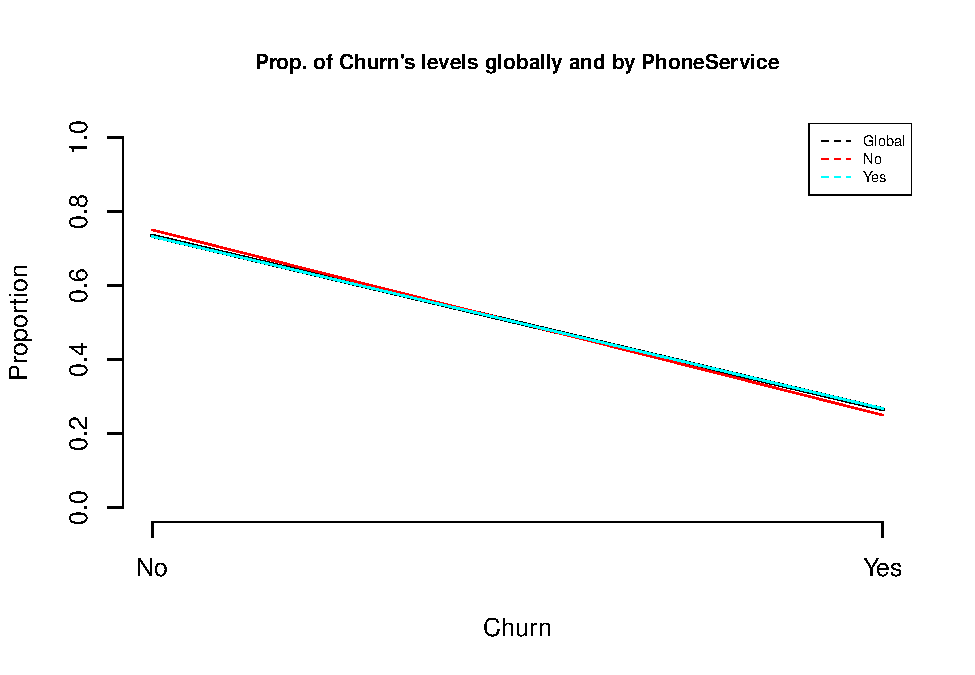
\includegraphics{AdriàCasanova-VíctorGarcia-ZhengyongJi_files/figure-latex/Karinas profiling method not hidden-11.pdf}
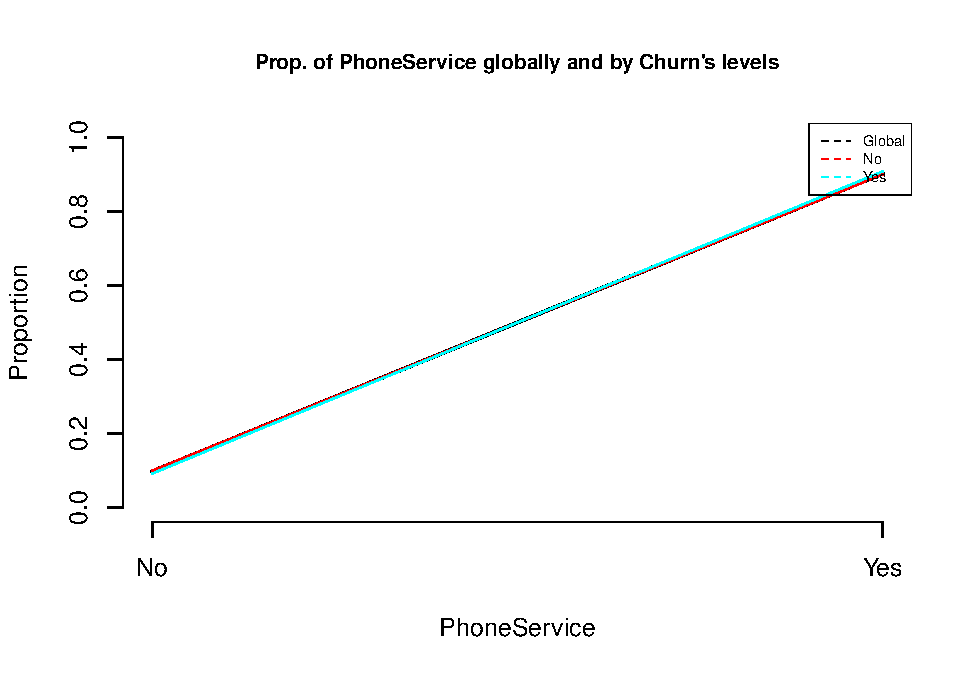
\includegraphics{AdriàCasanova-VíctorGarcia-ZhengyongJi_files/figure-latex/Karinas profiling method not hidden-12.pdf}

\begin{verbatim}
## [1] "Cross Table:"
##      P
##         No  Yes
##   No   512  170
##   Yes 4662 1699
## [1] "Distributions by columns:"
##      
## P            No       Yes
##   No  0.7507331 0.7329036
##   Yes 0.2492669 0.2670964
## [1] "Chi^2 test: "
## 
##  Pearson's Chi-squared test with Yates' continuity correction
## 
## data:  dades[, k] and as.factor(P)
## X-squared = 0.91503, df = 1, p-value = 0.3388
## 
## [1] "ValorTestXquali:"
## $rowpf
##      Xquali
## P             No        Yes
##   No  0.09895632 0.90104368
##   Yes 0.09095773 0.90904227
## 
## $vtest
##      Xquali
## P            No       Yes
##   No   1.002202 -1.002202
##   Yes -1.002202  1.002202
## 
## $pval
##      Xquali
## P            No       Yes
##   No  0.1581231 0.1581231
##   Yes 0.1581231 0.1581231
## 
## [1] "Variable MultipleLines"
## [1] "Categories="      "No"               "No phone service" "Yes"
\end{verbatim}

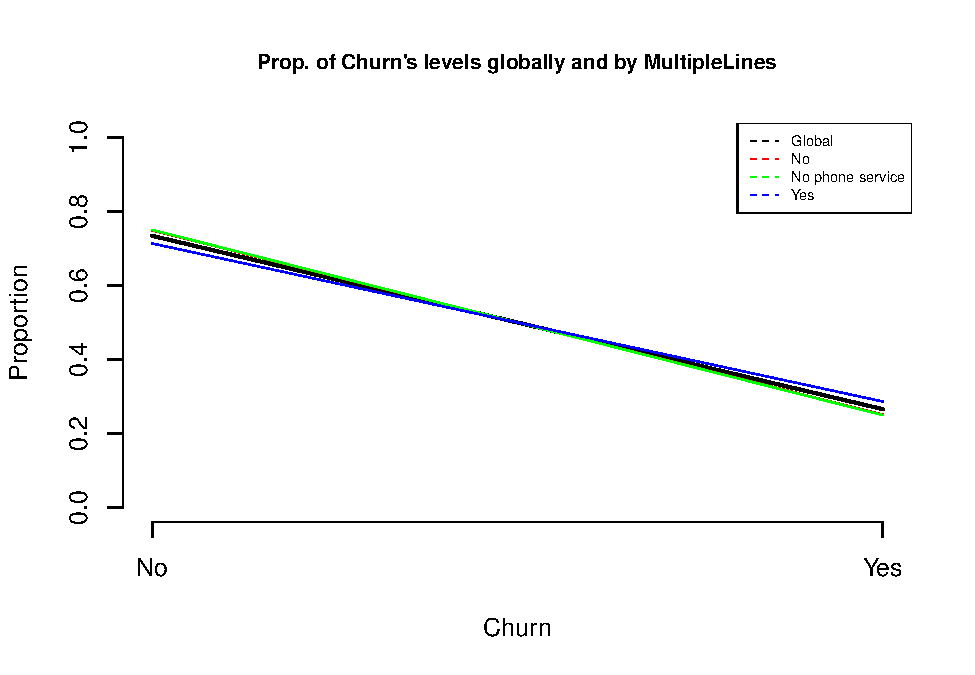
\includegraphics{AdriàCasanova-VíctorGarcia-ZhengyongJi_files/figure-latex/Karinas profiling method not hidden-13.pdf}
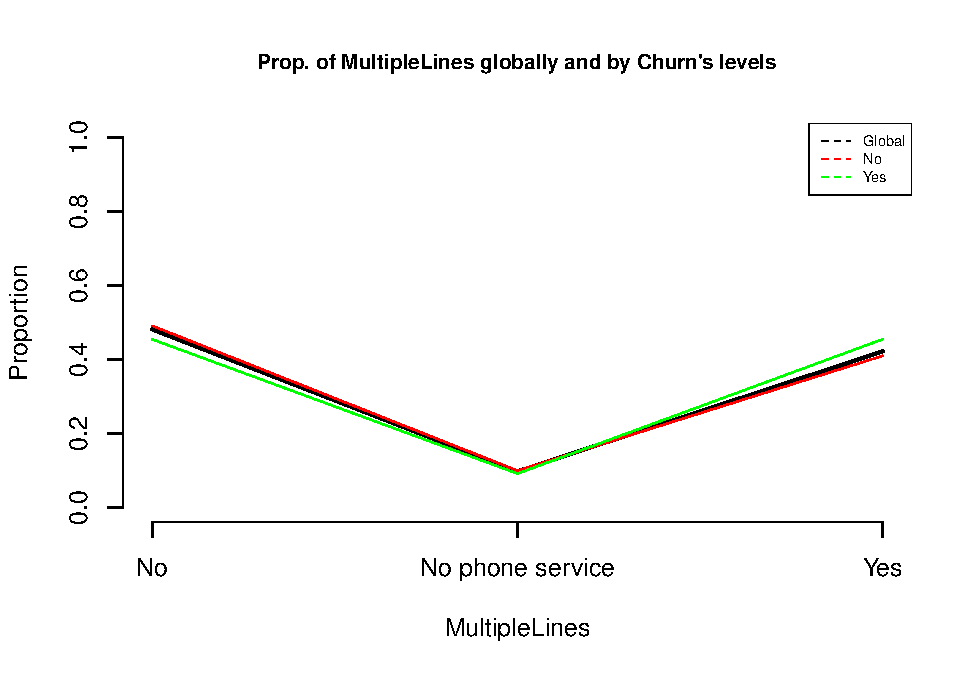
\includegraphics{AdriàCasanova-VíctorGarcia-ZhengyongJi_files/figure-latex/Karinas profiling method not hidden-14.pdf}

\begin{verbatim}
## [1] "Cross Table:"
##                   P
##                      No  Yes
##   No               2541  849
##   No phone service  512  170
##   Yes              2121  850
## [1] "Distributions by columns:"
##      
## P            No No phone service       Yes
##   No  0.7495575        0.7507331 0.7139010
##   Yes 0.2504425        0.2492669 0.2860990
## [1] "Chi^2 test: "
## 
##  Pearson's Chi-squared test
## 
## data:  dades[, k] and as.factor(P)
## X-squared = 11.33, df = 2, p-value = 0.003464
## 
## [1] "ValorTestXquali:"
## $rowpf
##      Xquali
## P             No No phone service        Yes
##   No  0.49110939       0.09895632 0.40993429
##   Yes 0.45425361       0.09095773 0.45478866
## 
## $vtest
##      Xquali
## P            No No phone service       Yes
##   No   2.733239         1.002202 -3.365474
##   Yes -2.733239        -1.002202  3.365474
## 
## $pval
##      Xquali
## P               No No phone service          Yes
##   No  0.0031357380     0.1581230658 0.0003820611
##   Yes 0.0031357380     0.1581230658 0.0003820611
## 
## [1] "Variable InternetService"
## [1] "Categories=" "DSL"         "Fiber optic" "No"
\end{verbatim}

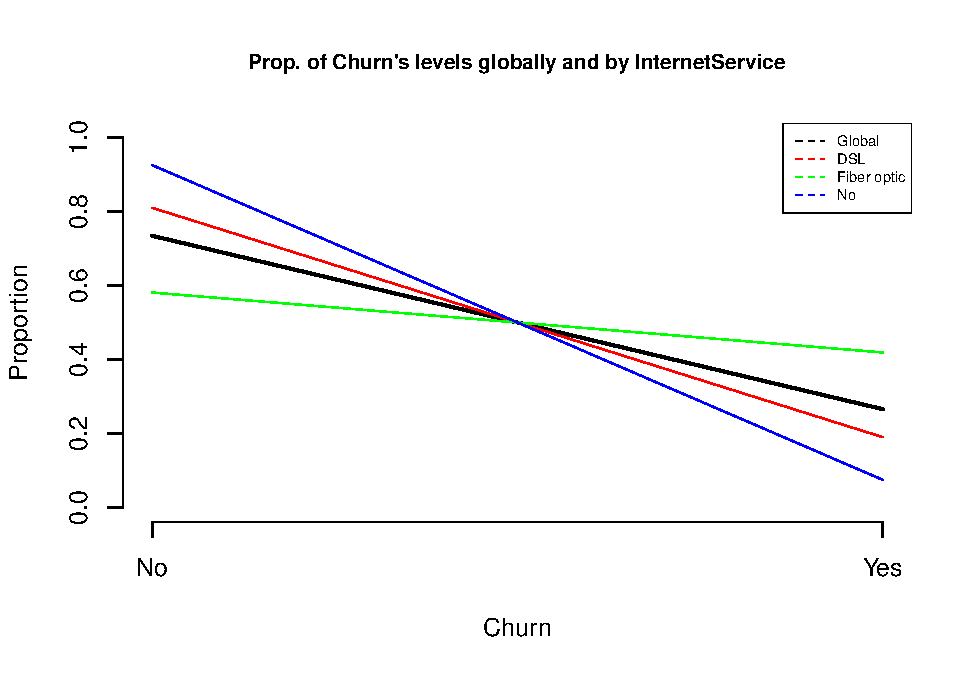
\includegraphics{AdriàCasanova-VíctorGarcia-ZhengyongJi_files/figure-latex/Karinas profiling method not hidden-15.pdf}
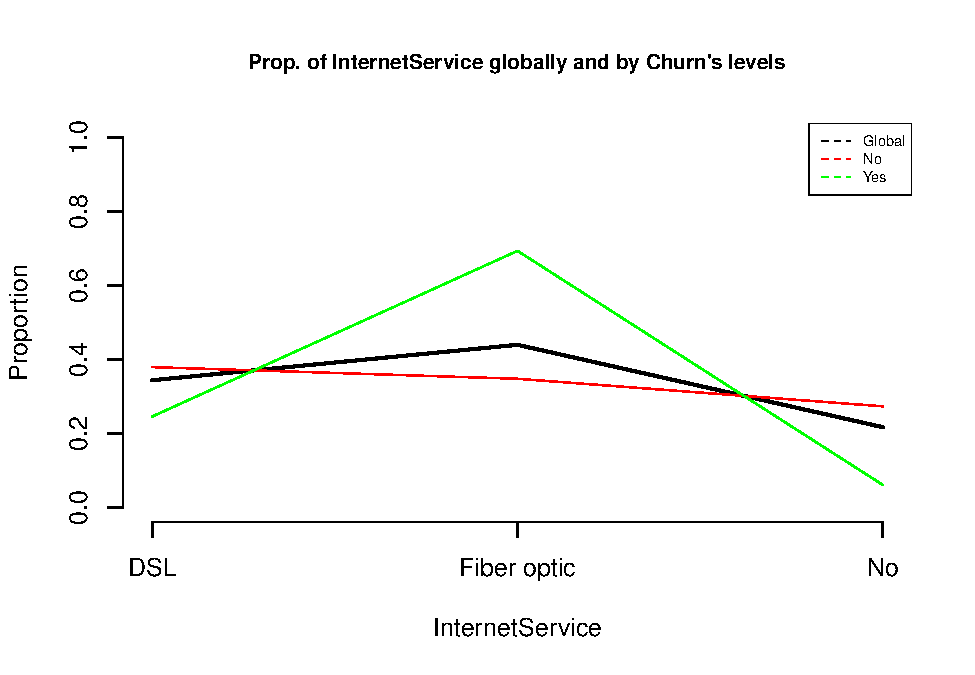
\includegraphics{AdriàCasanova-VíctorGarcia-ZhengyongJi_files/figure-latex/Karinas profiling method not hidden-16.pdf}

\begin{verbatim}
## [1] "Cross Table:"
##              P
##                 No  Yes
##   DSL         1962  459
##   Fiber optic 1799 1297
##   No          1413  113
## [1] "Distributions by columns:"
##      
## P           DSL Fiber optic        No
##   No  0.8104089   0.5810724 0.9259502
##   Yes 0.1895911   0.4189276 0.0740498
## [1] "Chi^2 test: "
## 
##  Pearson's Chi-squared test
## 
## data:  dades[, k] and as.factor(P)
## X-squared = 732.31, df = 2, p-value < 2.2e-16
## 
## [1] "ValorTestXquali:"
## $rowpf
##      Xquali
## P            DSL Fiber optic         No
##   No  0.37920371  0.34770004 0.27309625
##   Yes 0.24558587  0.69395399 0.06046014
## 
## $vtest
##      Xquali
## P           DSL Fiber optic        No
##   No   10.42434   -25.84981  19.12516
##   Yes -10.42434    25.84981 -19.12516
## 
## $pval
##      Xquali
## P               DSL   Fiber optic            No
##   No   9.598875e-26  0.000000e+00  7.795425e-82
##   Yes  0.000000e+00 1.222462e-147  0.000000e+00
## 
## [1] "Variable OnlineSecurity"
## [1] "Categories="         "No"                  "No internet service"
## [4] "Yes"
\end{verbatim}

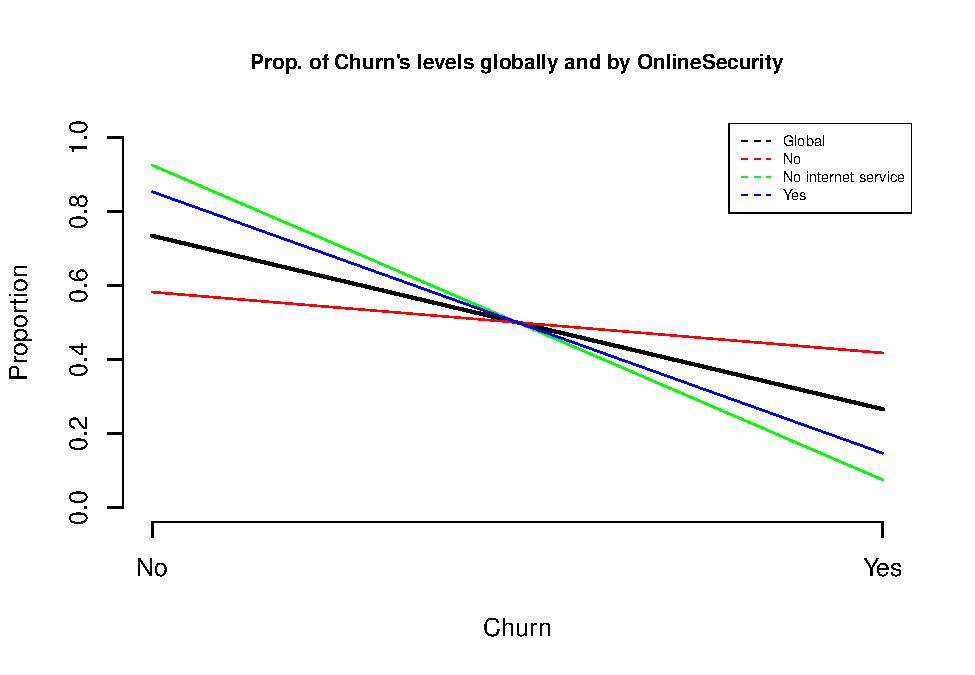
\includegraphics{AdriàCasanova-VíctorGarcia-ZhengyongJi_files/figure-latex/Karinas profiling method not hidden-17.pdf}
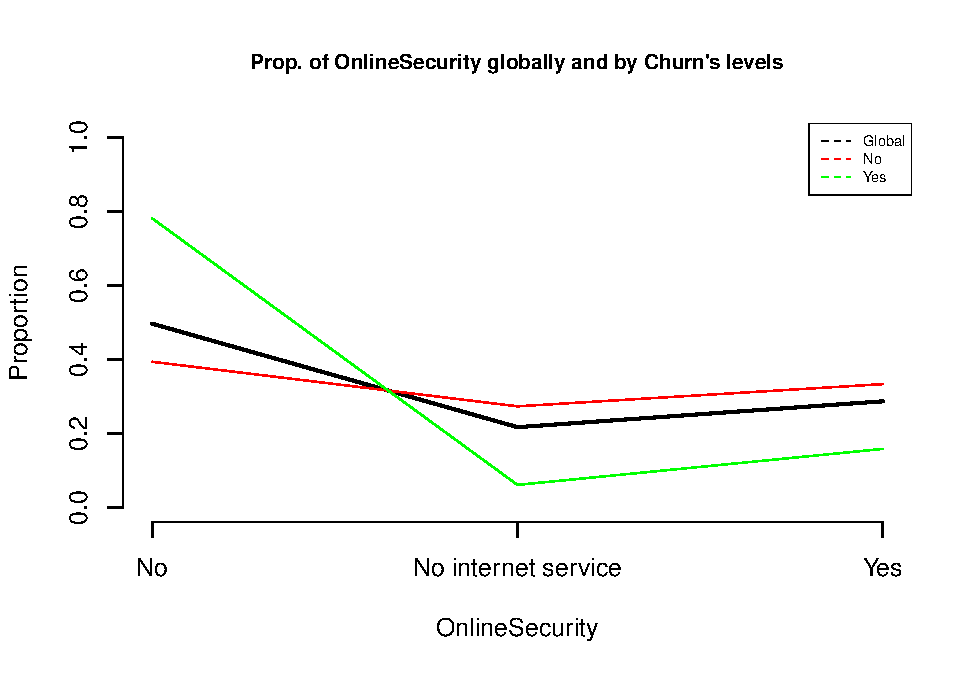
\includegraphics{AdriàCasanova-VíctorGarcia-ZhengyongJi_files/figure-latex/Karinas profiling method not hidden-18.pdf}

\begin{verbatim}
## [1] "Cross Table:"
##                      P
##                         No  Yes
##   No                  2037 1461
##   No internet service 1413  113
##   Yes                 1724  295
## [1] "Distributions by columns:"
##      
## P            No No internet service       Yes
##   No  0.5823328           0.9259502 0.8538881
##   Yes 0.4176672           0.0740498 0.1461119
## [1] "Chi^2 test: "
## 
##  Pearson's Chi-squared test
## 
## data:  dades[, k] and as.factor(P)
## X-squared = 850, df = 2, p-value < 2.2e-16
## 
## [1] "ValorTestXquali:"
## $rowpf
##      Xquali
## P             No No internet service        Yes
##   No  0.39369927          0.27309625 0.33320448
##   Yes 0.78170144          0.06046014 0.15783842
## 
## $vtest
##      Xquali
## P            No No internet service       Yes
##   No  -28.75497            19.12516  14.36975
##   Yes  28.75497           -19.12516 -14.36975
## 
## $pval
##      Xquali
## P                No No internet service           Yes
##   No   0.000000e+00        7.795425e-82  4.005837e-47
##   Yes 3.925582e-182        0.000000e+00  0.000000e+00
## 
## [1] "Variable OnlineBackup"
## [1] "Categories="         "No"                  "No internet service"
## [4] "Yes"
\end{verbatim}

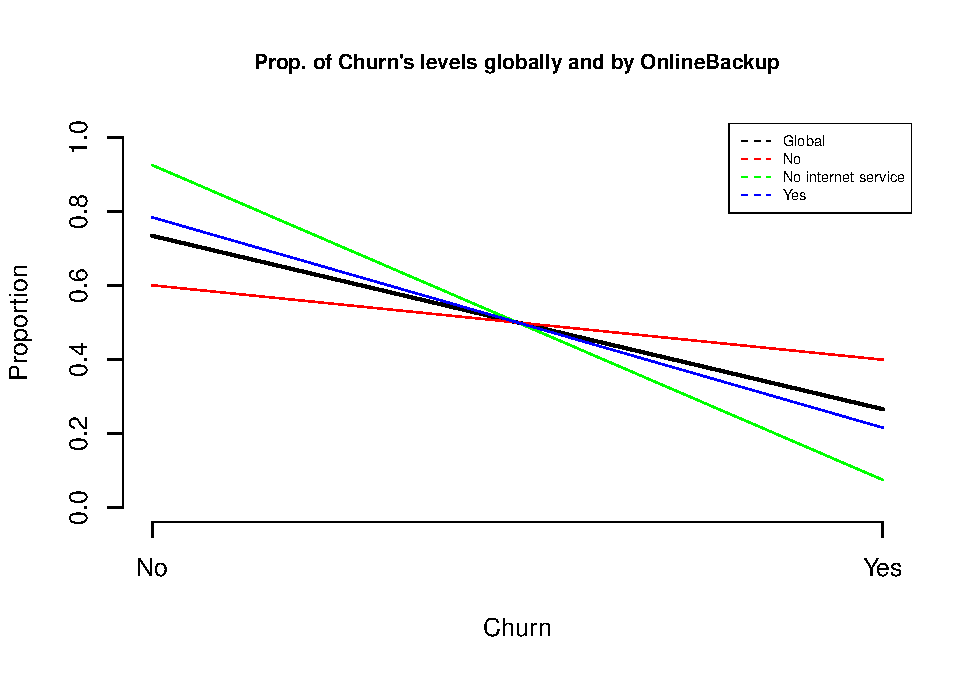
\includegraphics{AdriàCasanova-VíctorGarcia-ZhengyongJi_files/figure-latex/Karinas profiling method not hidden-19.pdf}
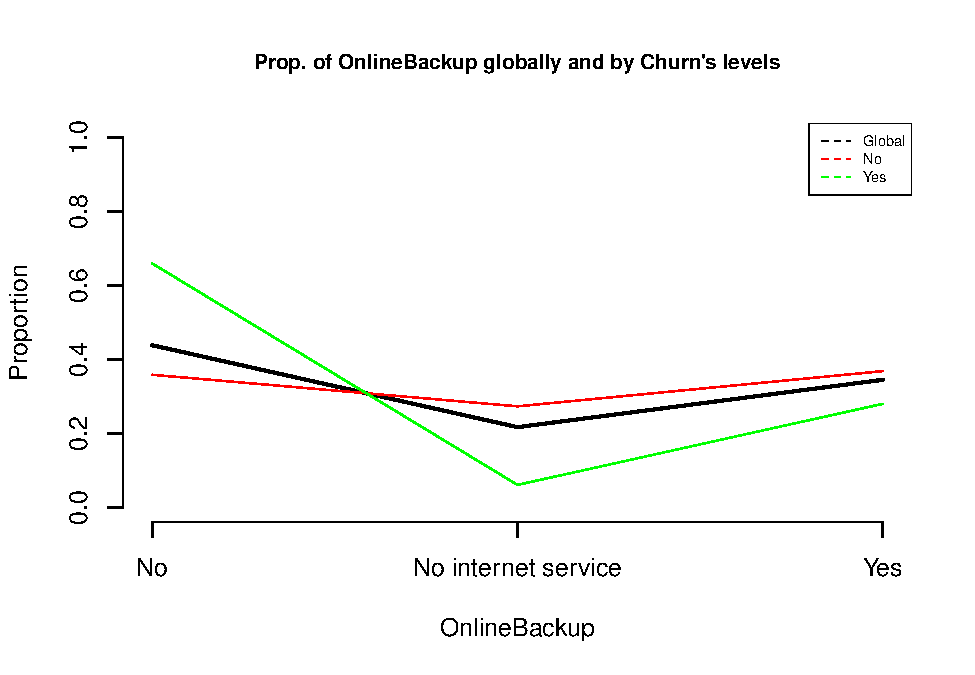
\includegraphics{AdriàCasanova-VíctorGarcia-ZhengyongJi_files/figure-latex/Karinas profiling method not hidden-20.pdf}

\begin{verbatim}
## [1] "Cross Table:"
##                      P
##                         No  Yes
##   No                  1855 1233
##   No internet service 1413  113
##   Yes                 1906  523
## [1] "Distributions by columns:"
##      
## P            No No internet service       Yes
##   No  0.6007124           0.9259502 0.7846851
##   Yes 0.3992876           0.0740498 0.2153149
## [1] "Chi^2 test: "
## 
##  Pearson's Chi-squared test
## 
## data:  dades[, k] and as.factor(P)
## X-squared = 601.81, df = 2, p-value < 2.2e-16
## 
## [1] "ValorTestXquali:"
## $rowpf
##      Xquali
## P             No No internet service        Yes
##   No  0.35852339          0.27309625 0.36838036
##   Yes 0.65971108          0.06046014 0.27982879
## 
## $vtest
##      Xquali
## P             No No internet service        Yes
##   No  -22.491687           19.125155   6.903041
##   Yes  22.491687          -19.125155  -6.903041
## 
## $pval
##      Xquali
## P                No No internet service           Yes
##   No   0.000000e+00        7.795425e-82  2.545045e-12
##   Yes 2.502984e-112        0.000000e+00  2.545075e-12
## 
## [1] "Variable DeviceProtection"
## [1] "Categories="         "No"                  "No internet service"
## [4] "Yes"
\end{verbatim}

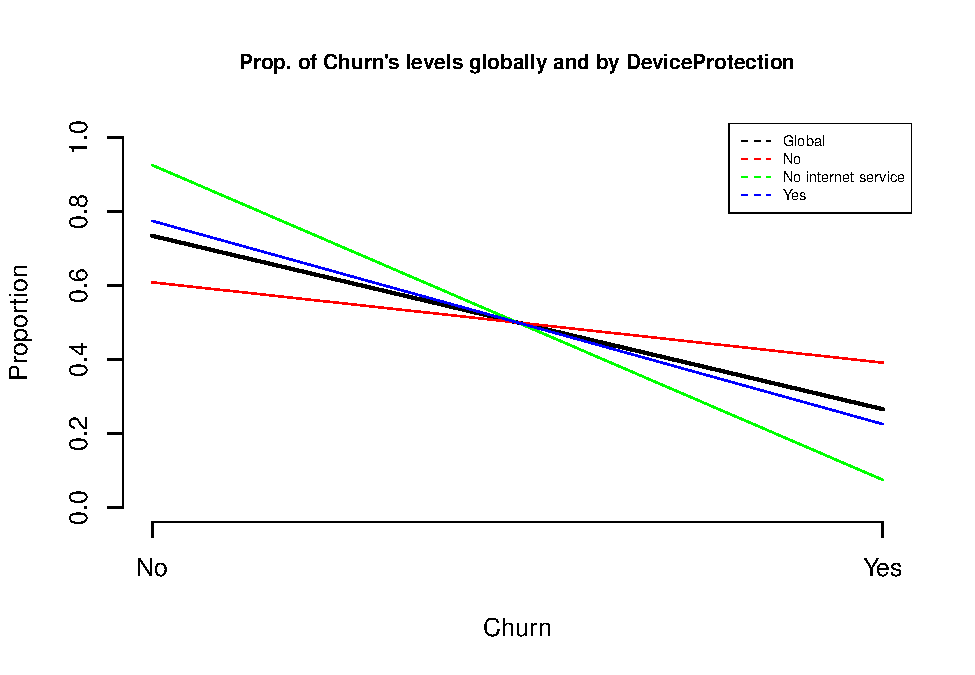
\includegraphics{AdriàCasanova-VíctorGarcia-ZhengyongJi_files/figure-latex/Karinas profiling method not hidden-21.pdf}
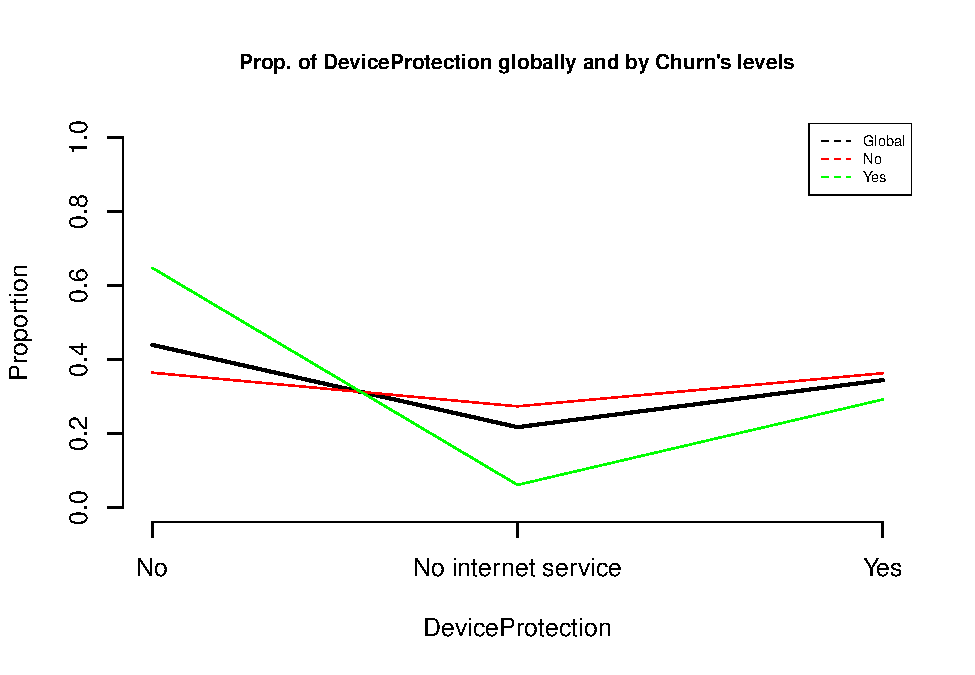
\includegraphics{AdriàCasanova-VíctorGarcia-ZhengyongJi_files/figure-latex/Karinas profiling method not hidden-22.pdf}

\begin{verbatim}
## [1] "Cross Table:"
##                      P
##                         No  Yes
##   No                  1884 1211
##   No internet service 1413  113
##   Yes                 1877  545
## [1] "Distributions by columns:"
##      
## P            No No internet service       Yes
##   No  0.6087237           0.9259502 0.7749794
##   Yes 0.3912763           0.0740498 0.2250206
## [1] "Chi^2 test: "
## 
##  Pearson's Chi-squared test
## 
## data:  dades[, k] and as.factor(P)
## X-squared = 558.42, df = 2, p-value < 2.2e-16
## 
## [1] "ValorTestXquali:"
## $rowpf
##      Xquali
## P             No No internet service        Yes
##   No  0.36412833          0.27309625 0.36277542
##   Yes 0.64794007          0.06046014 0.29159979
## 
## $vtest
##      Xquali
## P             No No internet service        Yes
##   No  -21.188888           19.125155   5.552301
##   Yes  21.188888          -19.125155  -5.552301
## 
## $pval
##      Xquali
## P                No No internet service           Yes
##   No   0.000000e+00        7.795425e-82  1.409671e-08
##   Yes 6.045963e-100        0.000000e+00  1.409671e-08
## 
## [1] "Variable TechSupport"
## [1] "Categories="         "No"                  "No internet service"
## [4] "Yes"
\end{verbatim}

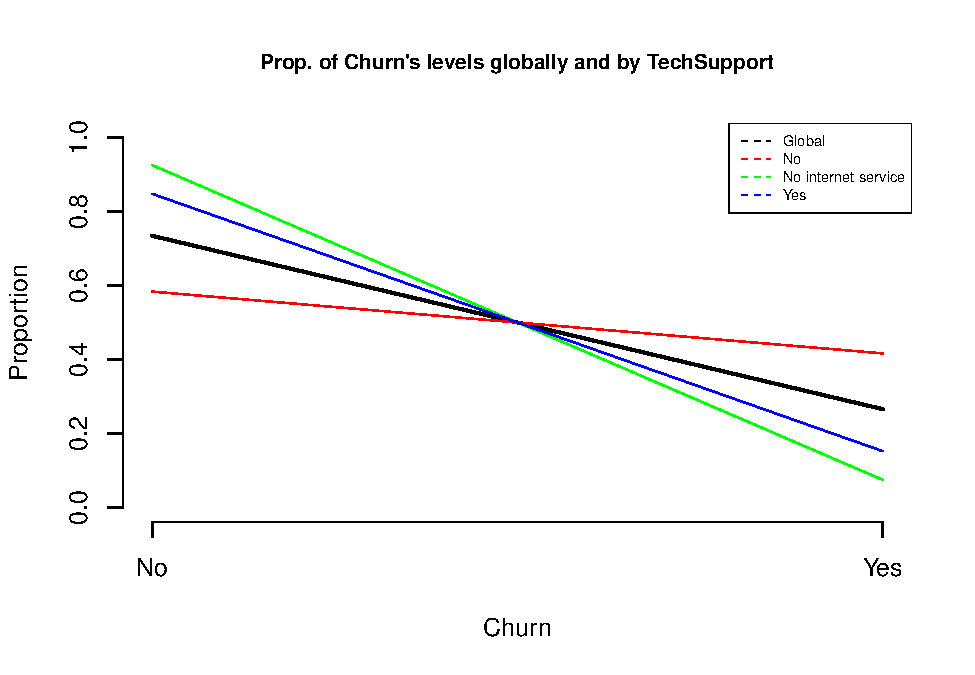
\includegraphics{AdriàCasanova-VíctorGarcia-ZhengyongJi_files/figure-latex/Karinas profiling method not hidden-23.pdf}
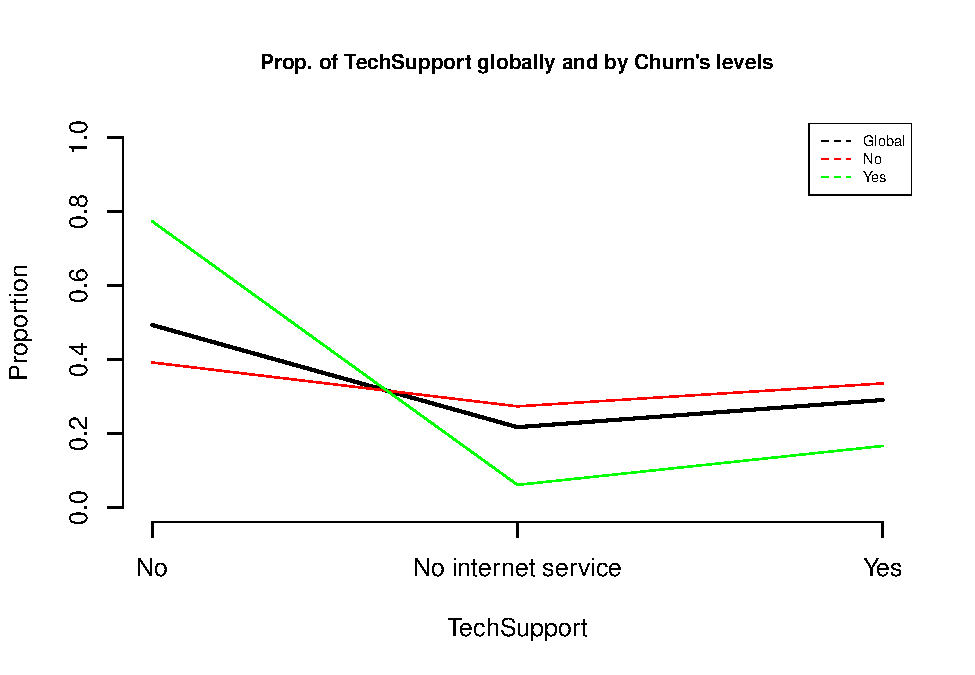
\includegraphics{AdriàCasanova-VíctorGarcia-ZhengyongJi_files/figure-latex/Karinas profiling method not hidden-24.pdf}

\begin{verbatim}
## [1] "Cross Table:"
##                      P
##                         No  Yes
##   No                  2027 1446
##   No internet service 1413  113
##   Yes                 1734  310
## [1] "Distributions by columns:"
##      
## P            No No internet service       Yes
##   No  0.5836453           0.9259502 0.8483366
##   Yes 0.4163547           0.0740498 0.1516634
## [1] "Chi^2 test: "
## 
##  Pearson's Chi-squared test
## 
## data:  dades[, k] and as.factor(P)
## X-squared = 828.2, df = 2, p-value < 2.2e-16
## 
## [1] "ValorTestXquali:"
## $rowpf
##      Xquali
## P             No No internet service        Yes
##   No  0.39176652          0.27309625 0.33513722
##   Yes 0.77367576          0.06046014 0.16586410
## 
## $vtest
##      Xquali
## P            No No internet service       Yes
##   No  -28.30547            19.12516  13.81983
##   Yes  28.30547           -19.12516 -13.81983
## 
## $pval
##      Xquali
## P                No No internet service           Yes
##   No   0.000000e+00        7.795425e-82  9.676286e-44
##   Yes 1.479823e-176        0.000000e+00  0.000000e+00
## 
## [1] "Variable StreamingTV"
## [1] "Categories="         "No"                  "No internet service"
## [4] "Yes"
\end{verbatim}

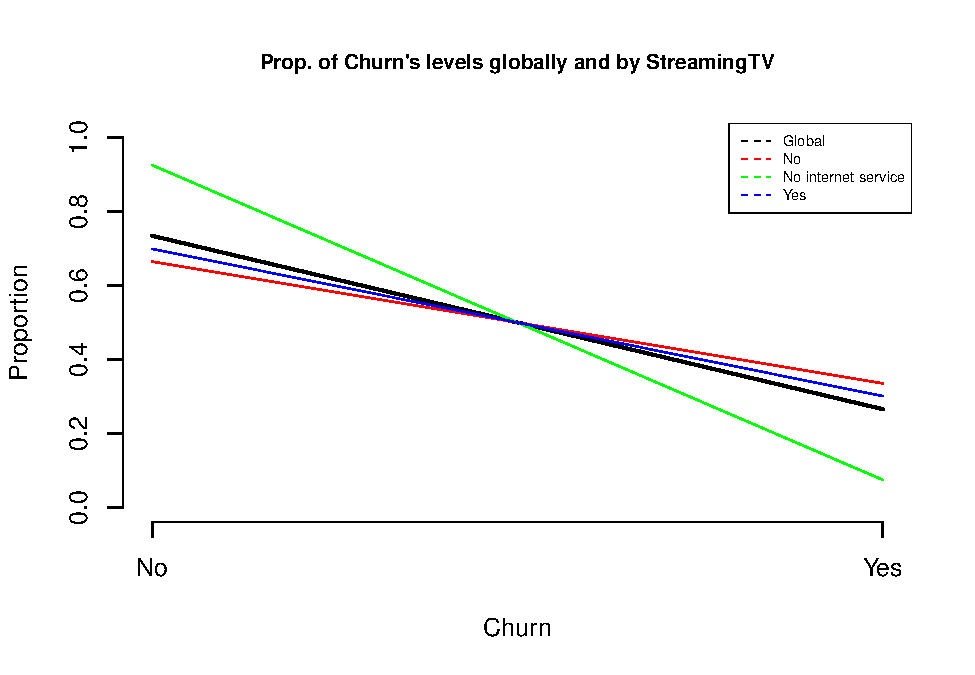
\includegraphics{AdriàCasanova-VíctorGarcia-ZhengyongJi_files/figure-latex/Karinas profiling method not hidden-25.pdf}
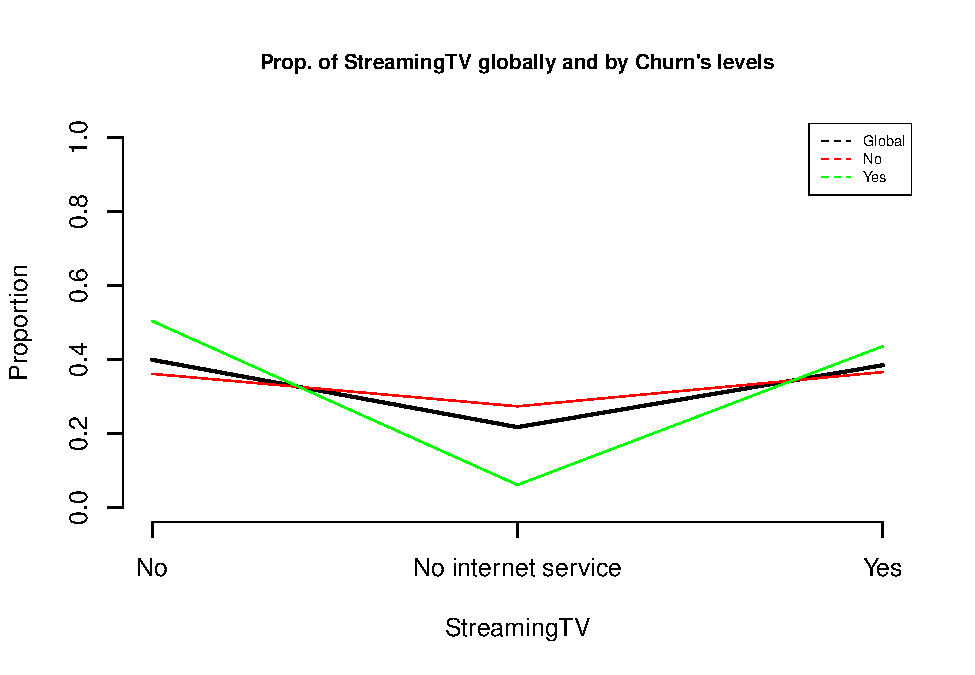
\includegraphics{AdriàCasanova-VíctorGarcia-ZhengyongJi_files/figure-latex/Karinas profiling method not hidden-26.pdf}

\begin{verbatim}
## [1] "Cross Table:"
##                      P
##                         No  Yes
##   No                  1868  942
##   No internet service 1413  113
##   Yes                 1893  814
## [1] "Distributions by columns:"
##      
## P            No No internet service       Yes
##   No  0.6647687           0.9259502 0.6992981
##   Yes 0.3352313           0.0740498 0.3007019
## [1] "Chi^2 test: "
## 
##  Pearson's Chi-squared test
## 
## data:  dades[, k] and as.factor(P)
## X-squared = 374.2, df = 2, p-value < 2.2e-16
## 
## [1] "ValorTestXquali:"
## $rowpf
##      Xquali
## P             No No internet service        Yes
##   No  0.36103595          0.27309625 0.36586780
##   Yes 0.50401284          0.06046014 0.43552702
## 
## $vtest
##      Xquali
## P             No No internet service        Yes
##   No  -10.818954           19.125155  -5.306236
##   Yes  10.818954          -19.125155   5.306236
## 
## $pval
##      Xquali
## P               No No internet service          Yes
##   No  0.000000e+00        7.795425e-82 5.595609e-08
##   Yes 1.399774e-27        0.000000e+00 5.595609e-08
## 
## [1] "Variable StreamingMovies"
## [1] "Categories="         "No"                  "No internet service"
## [4] "Yes"
\end{verbatim}

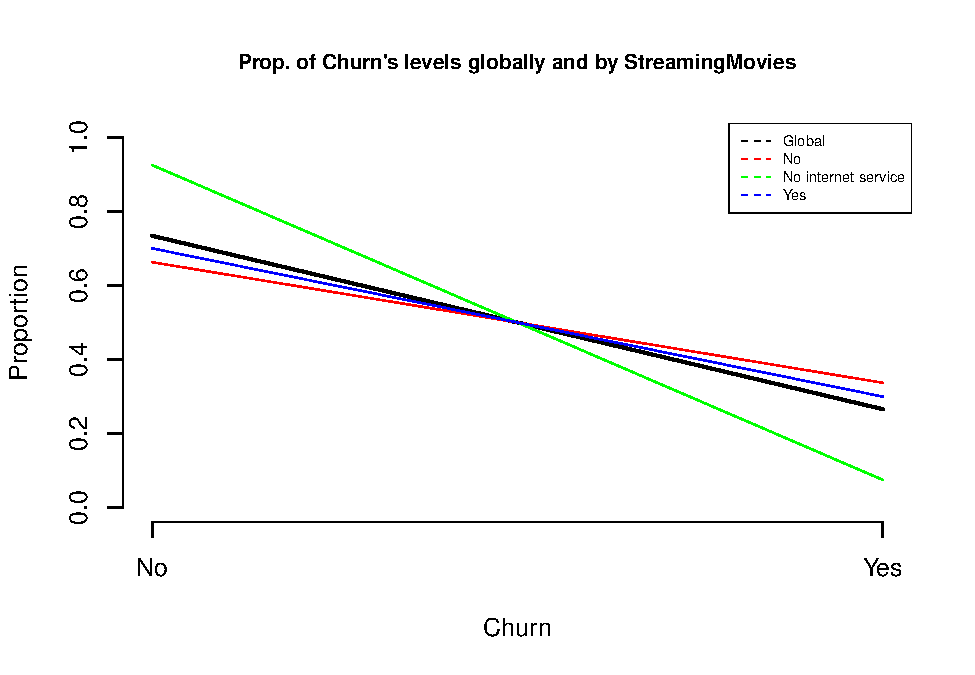
\includegraphics{AdriàCasanova-VíctorGarcia-ZhengyongJi_files/figure-latex/Karinas profiling method not hidden-27.pdf}
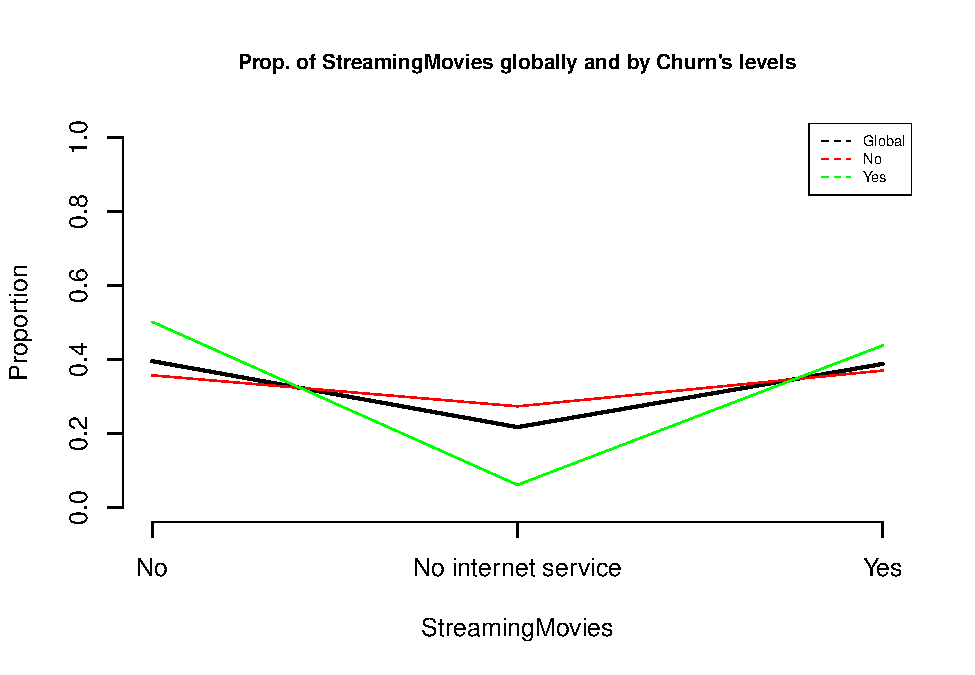
\includegraphics{AdriàCasanova-VíctorGarcia-ZhengyongJi_files/figure-latex/Karinas profiling method not hidden-28.pdf}

\begin{verbatim}
## [1] "Cross Table:"
##                      P
##                         No  Yes
##   No                  1847  938
##   No internet service 1413  113
##   Yes                 1914  818
## [1] "Distributions by columns:"
##      
## P            No No internet service       Yes
##   No  0.6631957           0.9259502 0.7005857
##   Yes 0.3368043           0.0740498 0.2994143
## [1] "Chi^2 test: "
## 
##  Pearson's Chi-squared test
## 
## data:  dades[, k] and as.factor(P)
## X-squared = 375.66, df = 2, p-value < 2.2e-16
## 
## [1] "ValorTestXquali:"
## $rowpf
##      Xquali
## P             No No internet service        Yes
##   No  0.35697719          0.27309625 0.36992656
##   Yes 0.50187266          0.06046014 0.43766720
## 
## $vtest
##      Xquali
## P             No No internet service        Yes
##   No  -10.980853           19.125155  -5.151298
##   Yes  10.980853          -19.125155   5.151298
## 
## $pval
##      Xquali
## P               No No internet service          Yes
##   No  0.000000e+00        7.795425e-82 1.293448e-07
##   Yes 2.362211e-28        0.000000e+00 1.293448e-07
## 
## [1] "Variable Contract"
## [1] "Categories="    "Month-to-month" "One year"       "Two year"
\end{verbatim}

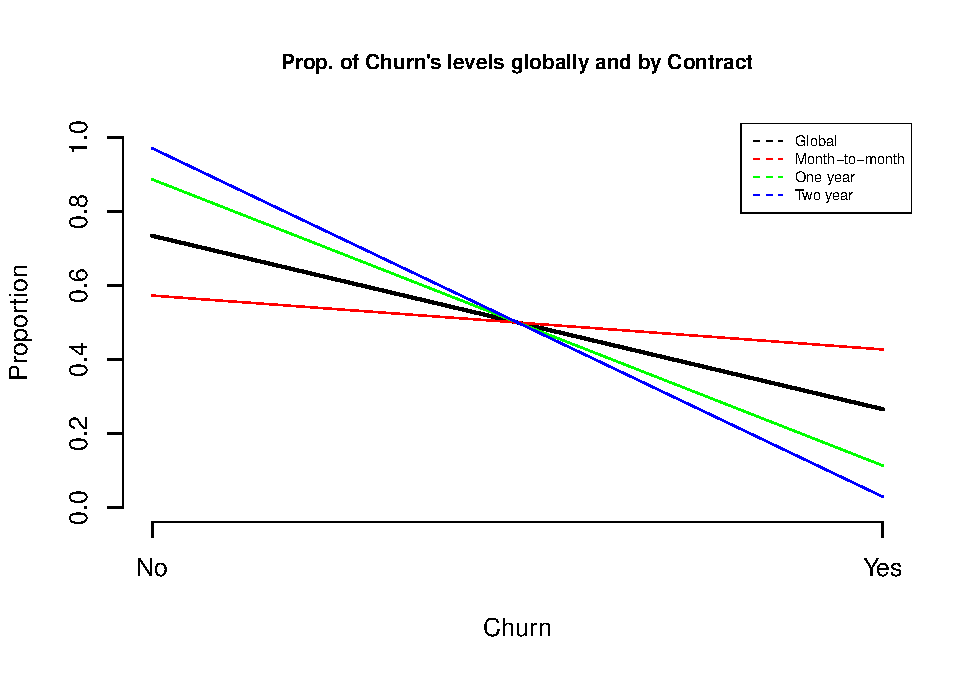
\includegraphics{AdriàCasanova-VíctorGarcia-ZhengyongJi_files/figure-latex/Karinas profiling method not hidden-29.pdf}
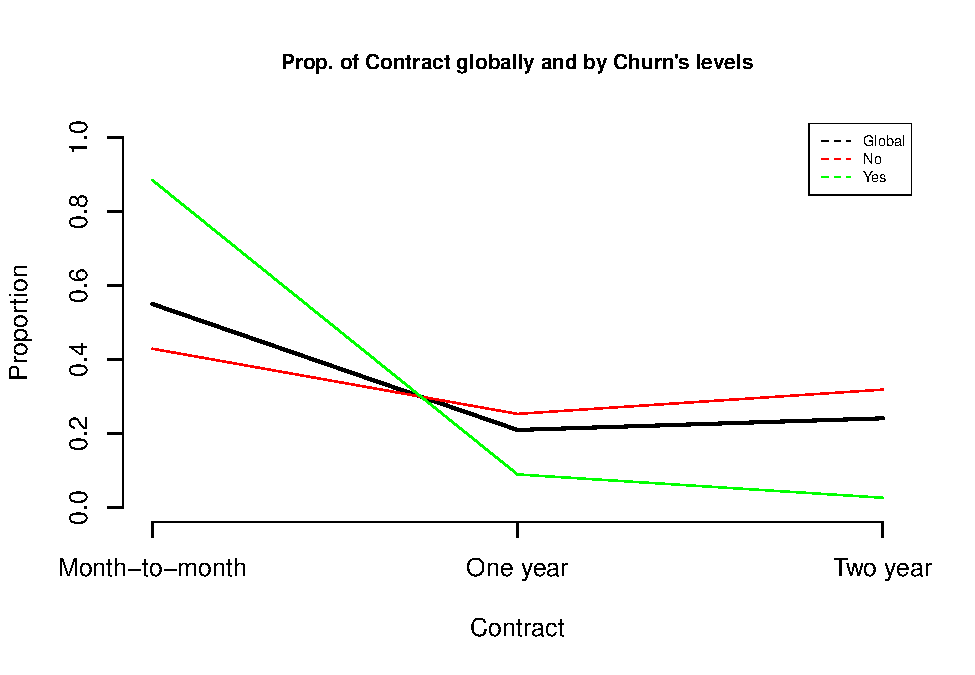
\includegraphics{AdriàCasanova-VíctorGarcia-ZhengyongJi_files/figure-latex/Karinas profiling method not hidden-30.pdf}

\begin{verbatim}
## [1] "Cross Table:"
##                 P
##                    No  Yes
##   Month-to-month 2220 1655
##   One year       1307  166
##   Two year       1647   48
## [1] "Distributions by columns:"
##      
## P     Month-to-month   One year   Two year
##   No      0.57290323 0.88730482 0.97168142
##   Yes     0.42709677 0.11269518 0.02831858
## [1] "Chi^2 test: "
## 
##  Pearson's Chi-squared test
## 
## data:  dades[, k] and as.factor(P)
## X-squared = 1184.6, df = 2, p-value < 2.2e-16
## 
## [1] "ValorTestXquali:"
## $rowpf
##      Xquali
## P     Month-to-month   One year   Two year
##   No      0.42906842 0.25260920 0.31832238
##   Yes     0.88550027 0.08881755 0.02568218
## 
## $vtest
##      Xquali
## P     Month-to-month  One year  Two year
##   No       -33.99728  14.92312  25.36589
##   Yes       33.99728 -14.92312 -25.36589
## 
## $pval
##      Xquali
## P     Month-to-month      One year      Two year
##   No    0.000000e+00  1.165649e-50 3.001022e-142
##   Yes  1.221803e-253  0.000000e+00  0.000000e+00
## 
## [1] "Variable PaperlessBilling"
## [1] "Categories=" "No"          "Yes"
\end{verbatim}

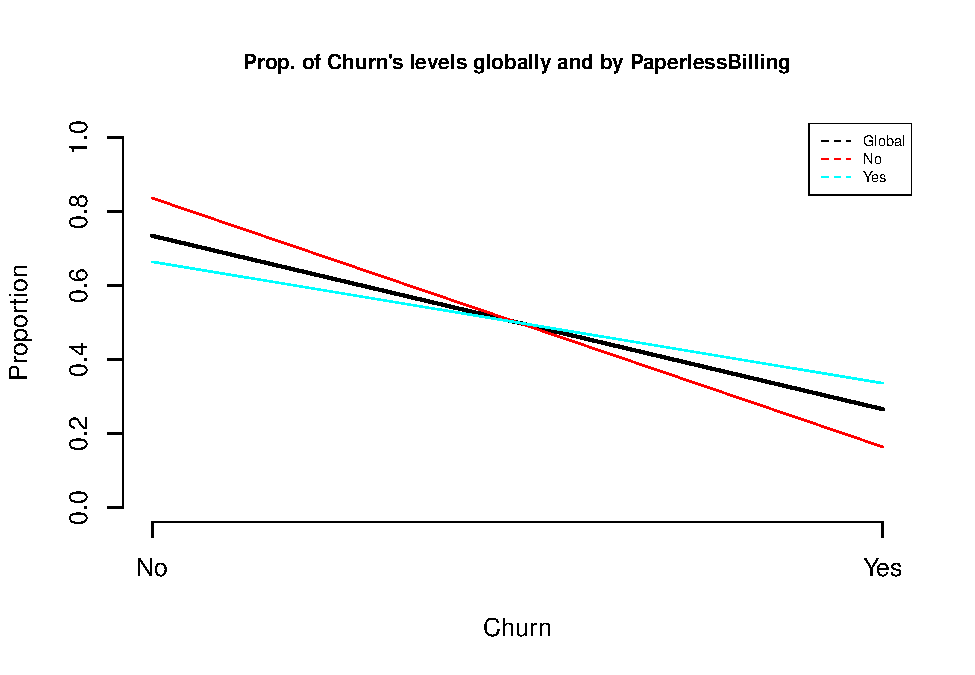
\includegraphics{AdriàCasanova-VíctorGarcia-ZhengyongJi_files/figure-latex/Karinas profiling method not hidden-31.pdf}
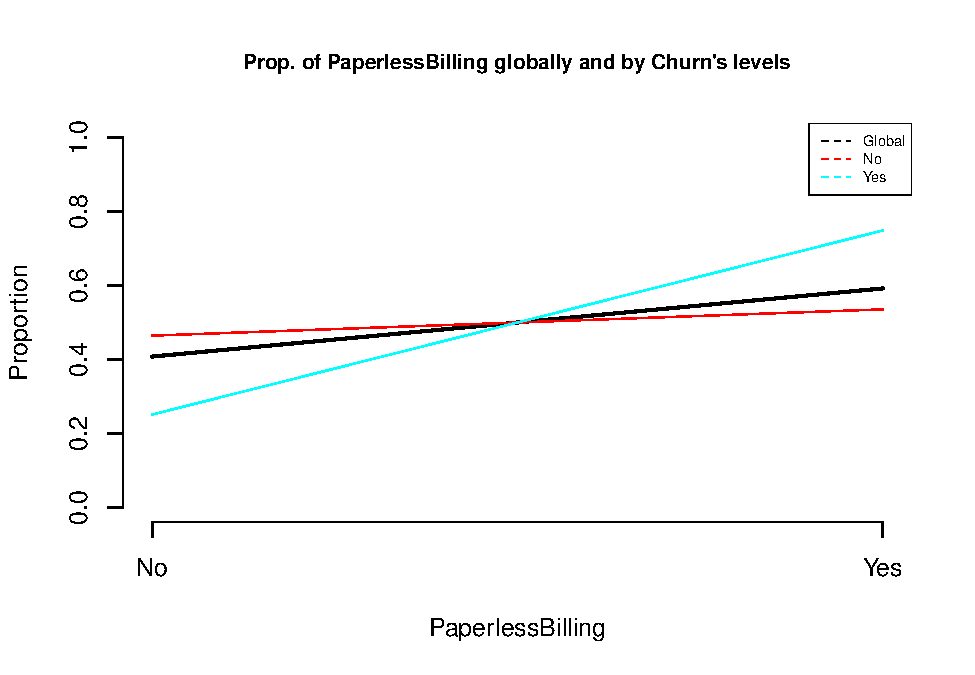
\includegraphics{AdriàCasanova-VíctorGarcia-ZhengyongJi_files/figure-latex/Karinas profiling method not hidden-32.pdf}

\begin{verbatim}
## [1] "Cross Table:"
##      P
##         No  Yes
##   No  2403  469
##   Yes 2771 1400
## [1] "Distributions by columns:"
##      
## P            No       Yes
##   No  0.8366992 0.6643491
##   Yes 0.1633008 0.3356509
## [1] "Chi^2 test: "
## 
##  Pearson's Chi-squared test with Yates' continuity correction
## 
## data:  dades[, k] and as.factor(P)
## X-squared = 258.28, df = 1, p-value < 2.2e-16
## 
## [1] "ValorTestXquali:"
## $rowpf
##      Xquali
## P            No       Yes
##   No  0.4644376 0.5355624
##   Yes 0.2509363 0.7490637
## 
## $vtest
##      Xquali
## P            No       Yes
##   No   16.09848 -16.09848
##   Yes -16.09848  16.09848
## 
## $pval
##      Xquali
## P               No          Yes
##   No  1.307299e-58 0.000000e+00
##   Yes 0.000000e+00 1.307299e-58
## 
## [1] "Variable PaymentMethod"
## [1] "Categories="               "Bank transfer (automatic)"
## [3] "Credit card (automatic)"   "Electronic check"         
## [5] "Mailed check"
\end{verbatim}

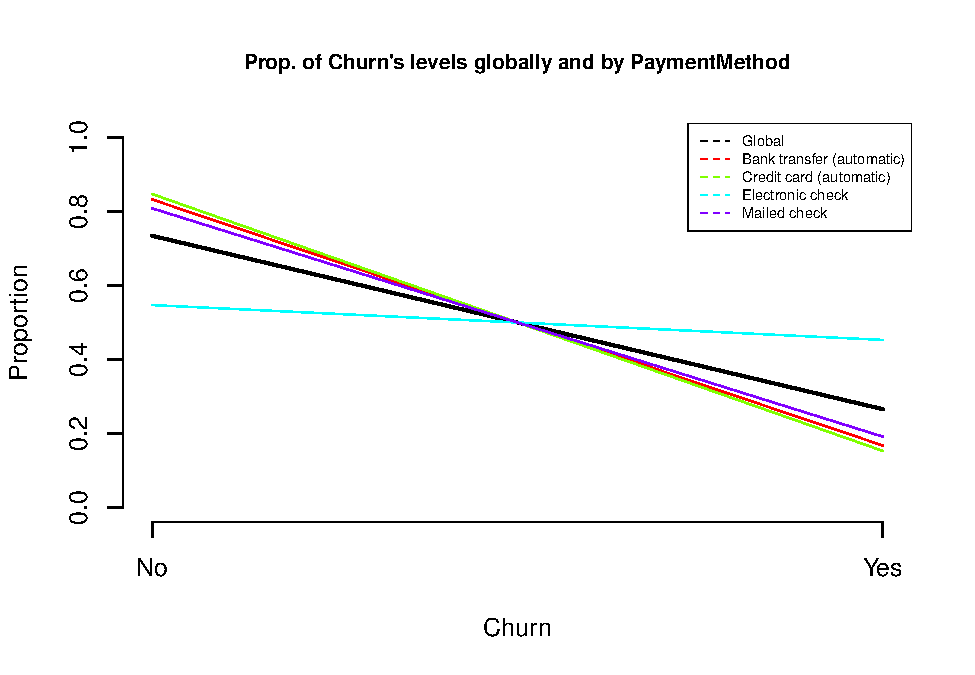
\includegraphics{AdriàCasanova-VíctorGarcia-ZhengyongJi_files/figure-latex/Karinas profiling method not hidden-33.pdf}
\includegraphics{AdriàCasanova-VíctorGarcia-ZhengyongJi_files/figure-latex/Karinas profiling method not hidden-34.pdf}

\begin{verbatim}
## [1] "Cross Table:"
##                            P
##                               No  Yes
##   Bank transfer (automatic) 1286  258
##   Credit card (automatic)   1290  232
##   Electronic check          1294 1071
##   Mailed check              1304  308
## [1] "Distributions by columns:"
##      
## P     Bank transfer (automatic) Credit card (automatic) Electronic check
##   No                  0.8329016               0.8475690        0.5471459
##   Yes                 0.1670984               0.1524310        0.4528541
##      
## P     Mailed check
##   No     0.8089330
##   Yes    0.1910670
## [1] "Chi^2 test: "
## 
##  Pearson's Chi-squared test
## 
## data:  dades[, k] and as.factor(P)
## X-squared = 648.14, df = 3, p-value < 2.2e-16
## 
## [1] "ValorTestXquali:"
## $rowpf
##      Xquali
## P     Bank transfer (automatic) Credit card (automatic) Electronic check
##   No                  0.2485504               0.2493235        0.2500966
##   Yes                 0.1380417               0.1241306        0.5730337
##      Xquali
## P     Mailed check
##   No     0.2520294
##   Yes    0.1647940
## 
## $vtest
##      Xquali
## P     Bank transfer (automatic) Credit card (automatic) Electronic check
##   No                   9.897550               11.270950       -25.337801
##   Yes                 -9.897550              -11.270950        25.337801
##      Xquali
## P     Mailed check
##   No      7.694261
##   Yes    -7.694261
## 
## $pval
##      Xquali
## P     Bank transfer (automatic) Credit card (automatic) Electronic check
##   No               2.132984e-23            9.129469e-30     0.000000e+00
##   Yes              0.000000e+00            0.000000e+00    6.123943e-142
##      Xquali
## P      Mailed check
##   No   7.115733e-15
##   Yes  7.105427e-15
## 
## [1] "Analysis by level of : MonthlyCharges"
\end{verbatim}

\includegraphics{AdriàCasanova-VíctorGarcia-ZhengyongJi_files/figure-latex/Karinas profiling method not hidden-35.pdf}
\includegraphics{AdriàCasanova-VíctorGarcia-ZhengyongJi_files/figure-latex/Karinas profiling method not hidden-36.pdf}

\begin{verbatim}
## [1] "Statistics by group:"
##    Min. 1st Qu.  Median    Mean 3rd Qu.    Max. 
##   18.25   25.10   64.42   61.27   88.40  118.75 
##    Min. 1st Qu.  Median    Mean 3rd Qu.    Max. 
##   18.85   56.15   79.65   74.44   94.20  118.35 
## [1] "p-valueANOVA: 8.59244933154708e-73"
## [1] "p-value Kruskal-Wallis: 3.31128554878381e-54"
## [1] "p-values ValorsTest: "
##           No          Yes 
## 0.000000e+00 1.861643e-58 
## [1] "Analysis by level of : TotalCharges"
\end{verbatim}

\includegraphics{AdriàCasanova-VíctorGarcia-ZhengyongJi_files/figure-latex/Karinas profiling method not hidden-37.pdf}
\includegraphics{AdriàCasanova-VíctorGarcia-ZhengyongJi_files/figure-latex/Karinas profiling method not hidden-38.pdf}

\begin{verbatim}
## [1] "Statistics by group:"
##    Min. 1st Qu.  Median    Mean 3rd Qu.    Max. 
##     0.0   572.9  1679.5  2549.9  4262.9  8672.5 
##    Min. 1st Qu.  Median    Mean 3rd Qu.    Max. 
##   18.85  134.50  703.55 1531.80 2331.30 8684.80 
## [1] "p-valueANOVA: 5.90258060907269e-75"
## [1] "p-value Kruskal-Wallis: 5.68430392462642e-83"
## [1] "p-values ValorsTest: "
##           No          Yes 
## 2.476582e-61 0.000000e+00 
## [1] "Variable c.tenure"
## [1] "Categories=" "(-1,18]"     "(18,36]"     "(36,54]"     "(54,72]"
\end{verbatim}

\includegraphics{AdriàCasanova-VíctorGarcia-ZhengyongJi_files/figure-latex/Karinas profiling method not hidden-39.pdf}
\includegraphics{AdriàCasanova-VíctorGarcia-ZhengyongJi_files/figure-latex/Karinas profiling method not hidden-40.pdf}

\begin{verbatim}
## [1] "Cross Table:"
##          P
##             No  Yes
##   (-1,18] 1520 1214
##   (18,36] 1011  297
##   (36,54]  969  213
##   (54,72] 1674  145
## [1] "Distributions by columns:"
##      
## P        (-1,18]    (18,36]    (36,54]    (54,72]
##   No  0.55596196 0.77293578 0.81979695 0.92028587
##   Yes 0.44403804 0.22706422 0.18020305 0.07971413
## [1] "Chi^2 test: "
## 
##  Pearson's Chi-squared test
## 
## data:  dades[, k] and as.factor(P)
## X-squared = 823.12, df = 3, p-value < 2.2e-16
## 
## [1] "ValorTestXquali:"
## $rowpf
##      Xquali
## P        (-1,18]    (18,36]    (36,54]    (54,72]
##   No  0.29377658 0.19540008 0.18728257 0.32354078
##   Yes 0.64954521 0.15890851 0.11396469 0.07758159
## 
## $vtest
##      Xquali
## P        (-1,18]    (18,36]    (36,54]    (54,72]
##   No  -27.050598   3.477112   7.269625  20.822929
##   Yes  27.050598  -3.477112  -7.269625 -20.822929
## 
## $pval
##      Xquali
## P           (-1,18]       (18,36]       (36,54]       (54,72]
##   No   0.000000e+00  2.534231e-04  1.802435e-13  1.341373e-96
##   Yes 1.879067e-161  2.534231e-04  1.801892e-13  0.000000e+00
## 
## [1] "Variable c.TotalCharges"
## [1] "Categories=" "(-1,2171]"   "(2171,4342]" "(4342,6514]" "(6514,8685]"
\end{verbatim}

\includegraphics{AdriàCasanova-VíctorGarcia-ZhengyongJi_files/figure-latex/Karinas profiling method not hidden-41.pdf}
\includegraphics{AdriàCasanova-VíctorGarcia-ZhengyongJi_files/figure-latex/Karinas profiling method not hidden-42.pdf}

\begin{verbatim}
## [1] "Cross Table:"
##              P
##                 No  Yes
##   (-1,2171]   2938 1368
##   (2171,4342]  982  288
##   (4342,6514]  819  156
##   (6514,8685]  435   57
## [1] "Distributions by columns:"
##      
## P     (-1,2171] (2171,4342] (4342,6514] (6514,8685]
##   No  0.6823038   0.7732283   0.8400000   0.8841463
##   Yes 0.3176962   0.2267717   0.1600000   0.1158537
## [1] "Chi^2 test: "
## 
##  Pearson's Chi-squared test
## 
## data:  dades[, k] and as.factor(P)
## X-squared = 182.13, df = 3, p-value < 2.2e-16
## 
## [1] "ValorTestXquali:"
## $rowpf
##      Xquali
## P      (-1,2171] (2171,4342] (4342,6514] (6514,8685]
##   No  0.56783920  0.18979513  0.15829146  0.08407422
##   Yes 0.73194222  0.15409310  0.08346709  0.03049759
## 
## $vtest
##      Xquali
## P      (-1,2171] (2171,4342] (4342,6514] (6514,8685]
##   No  -12.474952    3.441018    8.028134    7.788175
##   Yes  12.474952   -3.441018   -8.028134   -7.788175
## 
## $pval
##      Xquali
## P        (-1,2171]  (2171,4342]  (4342,6514]  (6514,8685]
##   No  0.000000e+00 2.897645e-04 4.948298e-16 3.399196e-15
##   Yes 5.113421e-36 2.897645e-04 4.440892e-16 3.441691e-15
## 
## [1] "Variable c.MonthlyCharges"
## [1] "Categories="    "(18,30.69]"     "(30.69,59.38]"  "(59.38,89.06]" 
## [5] "(89.06,118.75]"
\end{verbatim}

\includegraphics{AdriàCasanova-VíctorGarcia-ZhengyongJi_files/figure-latex/Karinas profiling method not hidden-43.pdf}
\includegraphics{AdriàCasanova-VíctorGarcia-ZhengyongJi_files/figure-latex/Karinas profiling method not hidden-44.pdf}

\begin{verbatim}
## [1] "Cross Table:"
##                 P
##                    No  Yes
##   (18,30.69]     1478  156
##   (30.69,59.38]   882  326
##   (59.38,89.06]  1554  763
##   (89.06,118.75] 1260  624
## [1] "Distributions by columns:"
##      
## P     (18,30.69] (30.69,59.38] (59.38,89.06] (89.06,118.75]
##   No  0.90452876    0.73013245    0.67069486     0.66878981
##   Yes 0.09547124    0.26986755    0.32930514     0.33121019
## [1] "Chi^2 test: "
## 
##  Pearson's Chi-squared test
## 
## data:  dades[, k] and as.factor(P)
## X-squared = 332.54, df = 3, p-value < 2.2e-16
## 
## [1] "ValorTestXquali:"
## $rowpf
##      Xquali
## P     (18,30.69] (30.69,59.38] (59.38,89.06] (89.06,118.75]
##   No  0.28565906    0.17046772    0.30034789     0.24352532
##   Yes 0.08346709    0.17442483    0.40823970     0.33386838
## 
## $vtest
##      Xquali
## P      (18,30.69] (30.69,59.38] (59.38,89.06] (89.06,118.75]
##   No   17.7490901    -0.3889736    -8.5089368     -7.5625505
##   Yes -17.7490901     0.3889736     8.5089368      7.5625505
## 
## $pval
##      Xquali
## P       (18,30.69] (30.69,59.38] (59.38,89.06] (89.06,118.75]
##   No  8.758458e-71  3.486478e-01  0.000000e+00   1.976197e-14
##   Yes 0.000000e+00  3.486478e-01  8.776773e-18   1.976207e-14
## 
## [1] "P.values per class: No"
##           gender    SeniorCitizen          Partner       Dependents 
##         0.00e+00         0.00e+00         0.00e+00         0.00e+00 
##     PhoneService    MultipleLines  InternetService   OnlineSecurity 
##         0.00e+00         0.00e+00         0.00e+00         0.00e+00 
##     OnlineBackup DeviceProtection      TechSupport      StreamingTV 
##         0.00e+00         0.00e+00         0.00e+00         0.00e+00 
##  StreamingMovies         Contract PaperlessBilling    PaymentMethod 
##         0.00e+00         0.00e+00         0.00e+00         0.00e+00 
##   MonthlyCharges         c.tenure   c.TotalCharges c.MonthlyCharges 
##         0.00e+00         0.00e+00         0.00e+00         0.00e+00 
##           tenure     TotalCharges 
##        2.08e-181         2.48e-61 
## [1] "P.values per class: Yes"
##           gender    SeniorCitizen          Partner       Dependents 
##         0.00e+00         0.00e+00         0.00e+00         0.00e+00 
##           tenure     PhoneService    MultipleLines  InternetService 
##         0.00e+00         0.00e+00         0.00e+00         0.00e+00 
##   OnlineSecurity     OnlineBackup DeviceProtection      TechSupport 
##         0.00e+00         0.00e+00         0.00e+00         0.00e+00 
##      StreamingTV  StreamingMovies         Contract PaperlessBilling 
##         0.00e+00         0.00e+00         0.00e+00         0.00e+00 
##    PaymentMethod     TotalCharges         c.tenure   c.TotalCharges 
##         0.00e+00         0.00e+00         0.00e+00         0.00e+00 
## c.MonthlyCharges   MonthlyCharges 
##         0.00e+00         1.86e-58
\end{verbatim}

\newpage

\hypertarget{complete-eda}{%
\subsection{Complete EDA}\label{complete-eda}}

\end{document}
